% Options for packages loaded elsewhere
% Options for packages loaded elsewhere
\PassOptionsToPackage{unicode}{hyperref}
\PassOptionsToPackage{hyphens}{url}
\PassOptionsToPackage{dvipsnames,svgnames,x11names}{xcolor}
\DocumentMetadata{%
  lang = en-us,
  pdfversion = 2.0,
  pdfstandard = ua-2,
  tagging = on,
  tagging-setup = {math/setup=mathml-SE}
}
\tagpdfsetup{activate, tabsorder=structure}
%
\documentclass[
  letterpaper,
  double,
  12pt,
  1.0in,
  seploa]{beavtex}
\usepackage{xcolor}
\usepackage{amsmath,amssymb}
\setcounter{secnumdepth}{5}
\usepackage{iftex}
\ifPDFTeX
  \usepackage[T1]{fontenc}
  \usepackage[utf8]{inputenc}
  \usepackage{textcomp} % provide euro and other symbols
\else % if luatex or xetex
  \usepackage{unicode-math} % this also loads fontspec
  \defaultfontfeatures{Scale=MatchLowercase}
  \defaultfontfeatures[\rmfamily]{Ligatures=TeX,Scale=1}
\fi
\usepackage{lmodern}
\ifPDFTeX\else
  % xetex/luatex font selection
\fi
% Use upquote if available, for straight quotes in verbatim environments
\IfFileExists{upquote.sty}{\usepackage{upquote}}{}
\IfFileExists{microtype.sty}{% use microtype if available
  \usepackage[]{microtype}
  \UseMicrotypeSet[protrusion]{basicmath} % disable protrusion for tt fonts
}{}
\makeatletter
\@ifundefined{KOMAClassName}{% if non-KOMA class
  \IfFileExists{parskip.sty}{%
    \usepackage{parskip}
  }{% else
    \setlength{\parindent}{0pt}
    \setlength{\parskip}{6pt plus 2pt minus 1pt}}
}{% if KOMA class
  \KOMAoptions{parskip=half}}
\makeatother
% Make \paragraph and \subparagraph free-standing
\makeatletter
\ifx\paragraph\undefined\else
  \let\oldparagraph\paragraph
  \renewcommand{\paragraph}{
    \@ifstar
      \xxxParagraphStar
      \xxxParagraphNoStar
  }
  \newcommand{\xxxParagraphStar}[1]{\oldparagraph*{#1}\mbox{}}
  \newcommand{\xxxParagraphNoStar}[1]{\oldparagraph{#1}\mbox{}}
\fi
\ifx\subparagraph\undefined\else
  \let\oldsubparagraph\subparagraph
  \renewcommand{\subparagraph}{
    \@ifstar
      \xxxSubParagraphStar
      \xxxSubParagraphNoStar
  }
  \newcommand{\xxxSubParagraphStar}[1]{\oldsubparagraph*{#1}\mbox{}}
  \newcommand{\xxxSubParagraphNoStar}[1]{\oldsubparagraph{#1}\mbox{}}
\fi
\makeatother


\usepackage{longtable,booktabs,array}
\usepackage{calc} % for calculating minipage widths
% Correct order of tables after \paragraph or \subparagraph
\usepackage{etoolbox}
\makeatletter
\patchcmd\longtable{\par}{\if@noskipsec\mbox{}\fi\par}{}{}
\makeatother
% Allow footnotes in longtable head/foot
\IfFileExists{footnotehyper.sty}{\usepackage{footnotehyper}}{\usepackage{footnote}}
\makesavenoteenv{longtable}
\usepackage{graphicx}
\makeatletter
\newsavebox\pandoc@box
\newcommand*\pandocbounded[1]{% scales image to fit in text height/width
  \sbox\pandoc@box{#1}%
  \Gscale@div\@tempa{\textheight}{\dimexpr\ht\pandoc@box+\dp\pandoc@box\relax}%
  \Gscale@div\@tempb{\linewidth}{\wd\pandoc@box}%
  \ifdim\@tempb\p@<\@tempa\p@\let\@tempa\@tempb\fi% select the smaller of both
  \ifdim\@tempa\p@<\p@\scalebox{\@tempa}{\usebox\pandoc@box}%
  \else\usebox{\pandoc@box}%
  \fi%
}
% Set default figure placement to htbp
\def\fps@figure{htbp}
\makeatother


% definitions for citeproc citations
\NewDocumentCommand\citeproctext{}{}
\NewDocumentCommand\citeproc{mm}{%
  \begingroup\def\citeproctext{#2}\cite{#1}\endgroup}
\makeatletter
 % allow citations to break across lines
 \let\@cite@ofmt\@firstofone
 % avoid brackets around text for \cite:
 \def\@biblabel#1{}
 \def\@cite#1#2{{#1\if@tempswa , #2\fi}}
\makeatother
\newlength{\cslhangindent}
\setlength{\cslhangindent}{1.5em}
\newlength{\csllabelwidth}
\setlength{\csllabelwidth}{3em}
\newenvironment{CSLReferences}[2] % #1 hanging-indent, #2 entry-spacing
 {\begin{list}{}{%
  \setlength{\itemindent}{0pt}
  \setlength{\leftmargin}{0pt}
  \setlength{\parsep}{0pt}
  % turn on hanging indent if param 1 is 1
  \ifodd #1
   \setlength{\leftmargin}{\cslhangindent}
   \setlength{\itemindent}{-1\cslhangindent}
  \fi
  % set entry spacing
  \setlength{\itemsep}{#2\baselineskip}}}
 {\end{list}}
\usepackage{calc}
\newcommand{\CSLBlock}[1]{\hfill\break\parbox[t]{\linewidth}{\strut\ignorespaces#1\strut}}
\newcommand{\CSLLeftMargin}[1]{\parbox[t]{\csllabelwidth}{\strut#1\strut}}
\newcommand{\CSLRightInline}[1]{\parbox[t]{\linewidth - \csllabelwidth}{\strut#1\strut}}
\newcommand{\CSLIndent}[1]{\hspace{\cslhangindent}#1}



\setlength{\emergencystretch}{3em} % prevent overfull lines

\providecommand{\tightlist}{%
  \setlength{\itemsep}{0pt}\setlength{\parskip}{0pt}}



 


\usepackage{tikz}                     % DAG
\usetikzlibrary{positioning,chains}   % DAG
\newtheorem{proposition}{Proposition} % Proposition 
\newtheorem{definition}{Definition}   % Definition 
\usepackage{algorithm}
\usepackage{algpseudocode}
\usepackage{graphicx}                 % Insert and adjust images
\usepackage{amsmath}
% \usepackage{amsthm}
\makeatletter
\@ifpackageloaded{bookmark}{}{\usepackage{bookmark}}
\makeatother
\makeatletter
\@ifpackageloaded{caption}{}{\usepackage{caption}}
\AtBeginDocument{%
\ifdefined\contentsname
  \renewcommand*\contentsname{Table of contents}
\else
  \newcommand\contentsname{Table of contents}
\fi
\ifdefined\listfigurename
  \renewcommand*\listfigurename{List of Figures}
\else
  \newcommand\listfigurename{List of Figures}
\fi
\ifdefined\listtablename
  \renewcommand*\listtablename{List of Tables}
\else
  \newcommand\listtablename{List of Tables}
\fi
\ifdefined\figurename
  \renewcommand*\figurename{Figure}
\else
  \newcommand\figurename{Figure}
\fi
\ifdefined\tablename
  \renewcommand*\tablename{Table}
\else
  \newcommand\tablename{Table}
\fi
}
\@ifpackageloaded{float}{}{\usepackage{float}}
\floatstyle{ruled}
\@ifundefined{c@chapter}{\newfloat{codelisting}{h}{lop}}{\newfloat{codelisting}{h}{lop}[chapter]}
\floatname{codelisting}{Listing}
\newcommand*\listoflistings{\listof{codelisting}{List of Listings}}
\makeatother
\makeatletter
\makeatother
\makeatletter
\@ifpackageloaded{caption}{}{\usepackage{caption}}
\@ifpackageloaded{subcaption}{}{\usepackage{subcaption}}
\makeatother
\usepackage{bookmark}
\IfFileExists{xurl.sty}{\usepackage{xurl}}{} % add URL line breaks if available
\urlstyle{same}
\hypersetup{
  pdftitle={Copula-Based Mixture Transition Distribution Models for Forecasting Skewed and Zero-Inflated Time Series: Methodology and Comparisons with Deep Learning LSTM Networks},
  pdfauthor={Frances Lin},
  colorlinks=true,
  linkcolor={blue},
  filecolor={Maroon},
  citecolor={Blue},
  urlcolor={Blue},
  pdfcreator={LaTeX via pandoc}}


\title{Copula-Based Mixture Transition Distribution Models for
Forecasting Skewed and Zero-Inflated Time Series: Methodology and
Comparisons with Deep Learning LSTM
Networks} % {An Analysis of Something}
\submitdate{November 5, 2025} % {January 1, 2013}
\author{Frances Lin} % {Joseph A. Student}

\degree{Doctor of Philosophy} % {Master of Science}
\commencementyear{2026} % {2013}
\doctype{Dissertation}

\department{Statistics} % {Nuclear Engineering and Radiation Health Physics}

\depttype{Department} % {School}

\depthead{Chair} % {Director}

\major{Statistics} % {Radiation Health Physics}

\advisor{Lisa Madsen} % {Jane R. Professor}
	\coadvisor{Charlotte Wickham}

\abstract{Real-world time series in domains such as energy, insurance,
and transportation often exhibit skewness and zero-inflation, which can
undermine model performance if not properly addressed. To tackle these
challenges, we develop the copula-based Gamma Mixture Transition
Distribution (Gamma MTD) model and its zero-inflated extension (ZIGamma
MTD) to capture high-order dependence, skewed distributions, and
semicontinuous patterns. The proposed framework is generalizable,
accommodating a wide range of marginal distributions and copula families
beyond the Gamma and ZIGamma specifications. Simulation studies show
promising results across various scenarios, demonstrating their
effectiveness and robustness. Continued development of probabilistic
frameworks for skewed and zero-inflated time series is crucial for
methodological advancement and for expanding their applicability across
a wider range of fields. While recent AI advances such as Recurrent
Neural Networks (RNNs) and Long Short-Term Memory (LSTM) networks
effectively capture nonlinear and long-range dependence, claims of LSTM
superiority can be misleading with inappropriate benchmarks, and prior
work has shown that probabilistic models such as MTD perform comparably
in predicting, for example, disease spread. To assess the relative
strengths and limitations of each approach, we compare the proposed
Gamma and ZIGamma MTD models with LSTM networks. Results from both
simulation and real-data applications show that MTD models achieve
higher predictive accuracy and greater robustness, albeit at the cost of
increased computational demands and more involved model design, whereas
LSTMs provide faster predictions but with lower accuracy. These findings
highlight the complementary strengths of flexible probabilistic models
and AI-driven neural architectures, suggesting opportunities for further
advancements that integrate both approaches to better model skewed and
zero-inflated time series.}

	\acknowledgements{First and foremost, I would like to thank my advisors,
Lisa Madsen and Charlotte Wickham, for their dedication, support, and
inspiration throughout the process. They have not only shaped me as a
researcher, but have also inspired me on a personal level through their
integrity, kindness, and diligence. I am grateful for all the support
they have given. I could not have made it this far without their
guidance, nor could I have asked for better advisors. I would also like
to thank my committee memebers, James Molyneux, Claudio Fuentes, and
Prasad Tadepalli, for the time they dedicated and for their valuable
feedback. I am also grateful to Xiaotian Zheng, whose models formed the
basis of our work. He has been incredibly generous with his time and
advice.

I am grateful to my family, my mom, dad, and brother, for their
occational financial support and for their patience and understanding
througout the journey. While I am privileged not to be the first in my
family to pursue a doctoral degree, the unique challenges of my path
have been shared and felt by all of us. I am grateful to my uncle, a
professor of statistics in Taiwan, for his lifelong guidence and
influence, and to Kate Huntington, a professor of geology at my
undergraduate university, for inspiring me and igniting my interest in
research. I am thankful to my friends, including my cohort, for their
emotional support and for always being there, from late-night talks and
fun hikes to ski trips and random food adventures. I am thankful to
Gauri, my friend, cohort, and roommmate of over five years, and to
Baloo, Gauri's dog, for making this experience more manageable. Last but
not least, I give special thanks to my partner, Joseph, for his timely
distractions and annoyances.

This journey has been a long one: from navigating the challenges of
remote work during COVID in 2020-2021, to supporting my grandma as she
battled a brain tumor and gradually lost her ability to communicate over
the years, the passing of our family dog, Collie, in 2024, swearing in
as a U.S. citizen later in the same year, and completing an internship
at Posit this summer. I would not have made it this far without the
support of the aforementioned people, as well as many others.}




\begin{document}
\frontmatter
\maketitle
\mainmatter
\bookmarksetup{startatroot}

\chapter{Introduction}\label{sec-intro}

\section{Motivation and Objective}\label{motivation-and-objective}

Modeling complex patterns in sequence data is a central task across
domains such as energy, insurance, and transportation. Real-world time
series often exhibit skewness and zero-inflation, which, if unaddressed,
undermine prediction accuracy. For example, wind speeds are typically
skewed, while medical expenditures, insurance claims, and transportation
safety measures may also include an excess of zeros. These features
highlight the need for flexible models capable of capturing both
continuous skewed behavior and semicontinuous, zero-inflated structures.
Figure~\ref{fig-windspeed} and Figure~\ref{fig-simu-zigamma} illustrate
the skewed and zero-inflated time series that motivate the design
choices.

Recent advances in artificial intelligence (AI) have introduced powerful
deep learning architectures, particularly Recurrent Neural Networks
(RNNs) and Long Short-Term Memory (LSTM) networks. These models
effectively capture nonlinear and long-range dependence in data,
offering fast predictions without explicit probabilistic assumptions.
Nevertheless, claims of LSTM superiority can be misleading when compared
against inappropriate benchmarks such as ARIMA models. In addition,
prior work has found comparable predictive performance between
probabilistic Mixture Transition Distribution (MTD) model and deep
learning LSTM network for disease spread. These considerations motivate
a more rigorous comparison of deep learning approaches with flexible
probabilistic models designed to handle nonlinear, non-Gaussian, and
zero-inflated dynamics, providing a more realistic benchmark than
traditional methods.

While deep learning methods offer powerful predictive capabilities,
classical statistical approaches remain indispensable, especially when
robustness, interpretability, and uncertainty quantification are
priorities. We propose the Gamma Mixture Transition Distribution (Gamma
MTD) and the Zero-Inflated Gamma MTD (ZIGamma MTD) models, which extend
the traditional MTD framework through a copula-based formulation. These
models provide flexible and interpretable frameworks for skewed and
zero-inflated time series, enabling accurate representation of both
continuous and semicontinuous dynamics commonly observed in real-world
applications, while also allowing a fair comparison with deep learning
methods such as LSTMs.

This dissertation develops the Gamma MTD and ZIGamma MTD models,
evaluates their predictive performance and robustness, and compares them
with modern deep learning approaches such as LSTMs. By integrating
insights from both probabilistic and AI-driven frameworks, this work
highlights their complementary strengths and limitations, providing a
clearer picture of their practical applications. We expand on these
points in the sections that follow.

\section{Data Challenges}\label{data-challenges}

To account for skewness and zero-inflation commonly observed in
real-world time series, we develop a copula-based Gamma MTD model and
its zero-inflated extension, ZIGamma MTD, providing a robust, flexible,
and interpretable framework for modeling such data type.

The Gamma MTD model extends the original MTD framework by incorporating
copulas into the transition kernels. This allows the dependence
structure to be modeled separately from the marginal distributions,
enabling the selection of copula families that effectively capture
complex dependence while maintaining flexibility in the choice of
marginals. As a result, the model offers enhanced modeling capabilities
and greater adaptability to diverse data characteristics.

The ZIGamma MTD model further extends the copula-based Gamma MTD to
handle zero-inflated data by reconstructing the marginal distribution.
By transforming semi-continuous distributions into fully continuous
ones, this approach overcomes the challenges posed by non-continuity in
the copula approach. As a result, the model preserves its effectiveness
in modeling dependence structures while retaining flexibility in the
choice of marginals.

By developing and evaluating the Gamma MTD and ZIGamma MTD models, this
work aims to provide a robust and flexible framework for modeling
complex time series, addressing both skewness and zero-inflation while
preserving interpretability and effectiveness.

\begin{figure}

\centering{

\pandocbounded{\includegraphics[keepaspectratio,alt={Time series of wind speeds for the Gamma MTD model}]{images/chapter1/windspeed.png}}

}

\caption{\label{fig-windspeed}Time series plot of observed hourly wind
speeds (m/s) at heights of (a) 50\,m, (b) 10\,m, and (c) 2\,m above
ground level at the Limon Wind Energy Center, Colorado, for the year
2024. Data sourced from MERRA-2 via the NASA GES DISC Earthdata API.}

\end{figure}%

\begin{figure}

\centering{

\pandocbounded{\includegraphics[keepaspectratio,alt={Time series of simulated values for the ZIGamma MTD model}]{images/chapter1/zigamma.png}}

}

\caption{\label{fig-simu-zigamma}Time series plot of observed values for
varying zero-inflated probability (a) \(P = 0.1\), (b) \(P = 0.5\) , and
(c) \(P = 0.7\). Data generated from a ZIGamma MTD model with mean,
scale, and threshold parameters \(\mu = 7\), \(\beta = 1\), and
\(\epsilon = 0.1\).}

\end{figure}%

\section{Modeling Approaches}\label{modeling-approaches}

To ensure a fair and balanced evaluation, we examine two complementary
modeling approaches: probabilistic MTD models and deep learning methods,
such as LSTM networks.

MTD models represent each conditional distribution as a mixture of \(l\)
transition kernels, weighting past lags probabilistically to capture
complex temporal dependence. They are particularly effective for
non-Gaussian, skewed, and zero-inflated data. The copula-based
formulation further enhances their ability to model continuous and
semicontinuous patterns.

Recurrent Neural Network (RNN) architectures, including LSTMs, model
temporal dependence by propagating recurrent units over time. These
networks learn internal states directly from data using backpropagation
through time (BPTT) without relying on explicit probabilistic
assumptions. LSTMs efficiently capture long-range nonlinear dependence,
making them well-suited for fast prediction on large-scale datasets.

Although both MTD models and LSTMs describe evolving dynamics, they
differ fundamentally. MTD models employ probabilistic transition
mechanisms, whereas LSTMs rely on deterministic, learned transformations
of hidden and cell states. This distinction has practical implications:
MTD models tend to provide higher predictive accuracy, improved
robustness, and greater interpretability, but at greater computational
cost and with more complex model design. LSTMs offer faster predictions
and simpler deployment, but with lower interpretability and potentially
reduced accuracy.

By combining insights from both classical and AI-driven frameworks, this
work aims to provide practical guidance for modeling time series with
complex, skewed, and zero-inflated patterns.

\section{Outline of the Dissertation
Chapters}\label{outline-of-the-dissertation-chapters}

The rest of the dissertation is organized as follows. In Part I, we
propose the copula-based Gamma MTD model, detailing its design,
estimation procedures, and predictive performance. In Part II, we extend
this framework to accommodate zero-inflated time series with the ZIGamma
MTD model, covering similar aspects of design, estimation, and
prediction. In Part III, we compare the MTD models with deep learning
approaches, specifically the Long Short-Term Memory (LSTM) networks,
evaluating predictive performance and robustness through simulation
studies and real-world data applications.

\part{Models for Forecasting Skewed Time Series}

\chapter{Introduction}\label{sec-ch1-intro}

Time series data consist of observations measured at regular time
intervals. In these data types, observations often exhibit temporal
dependence; that is, observations from recent time lags tend to be
similar. Examples of time series data are sensor readings, stock prices,
sale figures, energy production, weather data, and various other
metrics.

Time series models capture how past values contribute to the current
value and use this information to predict future values. In the
autoregressive (AR) model with order \(p\), for example, each current
value depends on all \(p\) past values, with fixed, deterministic
weights. The mixture transition distribution (MTD) model extends the AR
models to accommodate discrete, continuous, and mixed time series,
expanding its range of applications. The MTD model models each
conditional distribution as a mixture of transition kernels, with
random, stochastic weights.

The first MTD model was developed in 1985 to model high-order Markov
chains (\citeproc{ref-raftery1985model}{Raftery 1985a},
\citeproc{ref-raftery1985new}{1985b}), followed by several variant
models over the years. Our work builds upon the architecture of the MTD
model introduced in 2022 by Zheng et al.
(\citeproc{ref-zheng2022construction}{2022}). This model includes
various applications, such as the Gaussian MTD, Poisson MTD, negative
binomial MTD, and Lomax MTD regression models, extending beyond linear,
Gaussian dynamics. However, there are two limitations. First, under this
model framework, the transition kernel lacks component-varying
parameters. Second, for certain invariant marginal distributions, the
transition kernel may either require careful construction or can result
in a form that is not explicitly defined or too complex.

We propose to incorporate copulas into the transition kernels to address
the second limitation. Using copulas, dependence structures and marginal
distributions can be modeled separately, enabling a choice of copula
families that effectively capture data's dependence while allowing
flexibility in marginal selection. The proposed copula-based MTD model
enables flexible dependence modeling and accommodates any continuous
marginals, thereby enhancing modeling capabilities and flexibility.

The rest of the chapter is organized as follows. We review the MTD model
developed by Zheng et al. (\citeproc{ref-zheng2022construction}{2022})
in Chapter~\ref{sec-ch1-background}. We present the proposed model in
Chapter~\ref{sec-ch1-prop} and provide an overview of the MCMC algorithm
for parameter estimation in Chapter~\ref{sec-ch1-comp}. We present the
results of various simulations conducted to assess the accuracy and
performance of the proposed model in Chapter~\ref{sec-ch1-simu} and
discuss the model's predictive capabilities, including uncertainty
quantification, in Chapter~\ref{sec-ch1-pred}. Finally, we conclude with
a discussion in Chapter~\ref{sec-ch1-discussion}.
Appendix~\ref{sec-appendix-ch1-pkag} provides the instruction for
installing the extended \texttt{mtd} \texttt{R} package.

\chapter{Background}\label{sec-ch1-background}

The MTD model is a state space model. The MTD model was initially
developed in 1985 to model high-order Markov chains
(\citeproc{ref-raftery1985model}{Raftery 1985a},
\citeproc{ref-raftery1985new}{1985b}). On a finite state space, the
model offers a parsimonious approximation of higher-order Markov chains.
On a more general state space, the model can capture non-Gaussian and
nonlinear features, such as flat stretches, bursts, outliers, and change
points (\citeproc{ref-raftery1994change}{Raftery 1994};
\citeproc{ref-le1996modeling}{Le et al. 1996}). The class of MTD models
and their generalizations have diverse applications, including wind
power forecasting, social behavior analysis, DNA sequence modeling, and
forecasting of stock prices and inflation rates. A complete review of
the MTD model and its applications can be found in Berchtold and Raftery
(\citeproc{ref-berchtold2002mixture}{2002}). Recent applications extend
to the modeling of crime incidents and precipitation patterns
(\citeproc{ref-zheng2022construction}{Zheng et al. 2022}) and the
network analysis of financial markets
(\citeproc{ref-damico2023network}{D'Amico et al. 2023}). Although the
MTD model has primarily been used for modeling time series, its
generalizations has also demonstrated success in modeling spatial data.
Some applications within the spatial context can be found in Berchtold
(\citeproc{ref-berchtold2001estimation}{2001}), Zheng et al.
(\citeproc{ref-zheng2023nnmp}{2023b}), and Zheng et al.
(\citeproc{ref-zheng2023nnmpdiscrete}{2023a}).

\section{Mixture Transition Distribution Models for Time
Series}\label{mixturetransitiondistributionmodels}

In the general MTD model framework, the joint data distribution over a
directed acyclic graph (DAG) is modeled as a weighted combination of
first-order component densities or transition kernels. A DAG simplifies
complex relationships in the data, enabling flexible and parsimonious
multivariate non-Gaussian modeling. Let \(\{ X_t: t \in \mathbb{N} \}\)
be a time series, represented by a sequence of random variables in an
arbitrary state space and \(f(\textbf{x})\), where
\(\textbf{x} = {(X_1,..., X_t)}^T\), be the joint distribution of
\(X_1\) to \(X_t\). By applying the chain rule of probability theory and
constructing the model on a DAG, the joint distribution of \(X_1\) to
\(X_t\) can be factorized into a product of conditional distributions as

\begin{equation}
f(\textbf{x}) = f(x_1) \prod_{t=2}^t f(x_t | \textbf{x}^{t-1}). 
\label{eq:joint_distribution}
\end{equation}

\(f(x_t | \textbf{x}^{t-1})\) is the conditional probability density
function (pdf) of current value \(X_t\) given all of its past values
\(\textbf{X}^{t-1} = \textbf{x}^{t-1}\), where
\(\textbf{X}^{t-1} = \{X_i: i \leq t - 1 \}\) and
\(\textbf{x}^{t-1} = \{x_i: i \leq t - 1 \}\). The joint distribution in
\eqref{eq:joint_distribution} corresponds to a directed graphical model
(Jordan (\citeproc{ref-jordan2004graphical}{2004}); also known as a
Bayesian network), where the conditional independence structure among
the random variables is encoded by a DAG. Figure \ref{Linear} and
\ref{DAG} provide visual illustrations of the linear and directed
relationships between \(X_1\) through \(X_t\) on a DAG, respectively. In
Figure \ref{DAG}, let \(X_1, ..., X_t\) be vertices or nodes in a graph.
The set \(\textbf{X}^{t-1}\), which consists of nodes that have directed
edges pointed to \(X_t\), is called the parent or conditioning set of
\(X_t\).

% Figure 1
\begin{figure}[htbp]  % Figure environment for adding caption
    \centering     % Center the diagram
    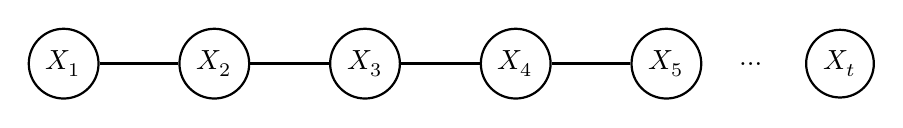
\begin{tikzpicture}[
    item/.style={circle, draw, thick, align=center},  % Style for the nodes (circles)
    itemc/.style={item, on chain, join},             % Style for the nodes in the chain
    start chain=going right,                         % Nodes arranged horizontally
    every join/.style={very thick}           % Style for the arrows (very thick, with arrowheads)
    ]

    % Define the chain of nodes X1 to X4
    \node[itemc] (X1) {$X_1$};
    \node[itemc] (X2) {$X_2$};
    \node[itemc] (X3) {$X_3$};
    \node[itemc] (X4) {$X_4$};
    \node[itemc] (X5) {$X_5$};

    % Add nodes for ... X_t
    \node[right=1em of X5] (dots) {$\dots$};
    \node[item, right=1em of dots] (Xt) {$X_t$}; 

    \end{tikzpicture}
    \caption{Relationships between $X_1, X_2, X_3, X_4, X_5, ..., X_t$. The joint distribution is $f(\textbf{x}) = f(x_1, x_2, x_3, ..., x_t)$.}
    \label{Linear}
\end{figure}

% Figure 2
\begin{figure}[htbp]  
    \centering  
    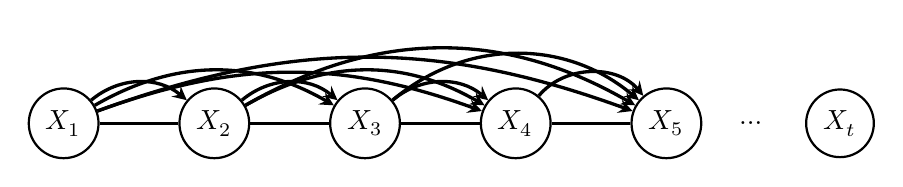
\begin{tikzpicture}[
    item/.style={circle, draw, thick, align=center},  % Style for the nodes (circles)
    itemc/.style={item, on chain, join},             % Style for the nodes in the chain
    start chain=going right,                         % Nodes arranged horizontally
    every join/.style={very thick},          % Style for the straight arrows
    >={stealth}                                      % Arrowhead style
    ]

    % Define the chain of nodes X1 to X5
    \node[itemc] (X1) {$X_1$};
    \node[itemc] (X2) {$X_2$};
    \node[itemc] (X3) {$X_3$};
    \node[itemc] (X4) {$X_4$};
    \node[itemc] (X5) {$X_5$};

    % Add nodes for ... X_t
    \node[right=1em of X5] (dots) {$\dots$};
    \node[item, right=1em of dots] (Xt) {$X_t$}; 

    % Add curved arrows for the directed relationships
    % X5 has arrows from X1, X2, X3, and X4
    \draw[->, bend left=20, very thick] (X1) to (X5);
    \draw[->, bend left=30, very thick] (X2) to (X5);
    \draw[->, bend left=40, very thick] (X3) to (X5);
    \draw[->, bend left=50, very thick] (X4) to (X5);

    % X4 has arrows from X1, X2, and X3
    \draw[->, bend left=20, very thick] (X1) to (X4);
    \draw[->, bend left=30, very thick] (X2) to (X4);
    \draw[->, bend left=40, very thick] (X3) to (X4);

    % X3 has arrows from X1 and X2
    \draw[->, bend left=30, very thick] (X1) to (X3);
    \draw[->, bend left=40, very thick] (X2) to (X3);

    % X2 has an arrow from X1
    \draw[->, bend left=40, very thick] (X1) to (X2);

    \end{tikzpicture}
    \caption{Directed relationships between $X_1, X_2, X_3, X_4, X_5, ..., X_t$ on a DAG. The joint distribution is factored as $f(\textbf{x}) = f(x_1) f(x_2 | x_1) f(x_3 | x_1, x_2) \cdots f(x_t | x_1, ..., x_{t-1})$.}
    \label{DAG}
\end{figure}

As \(t\) increases, the size of the conditioning set of \(X_t\) can
become notably large. Zheng et al.
(\citeproc{ref-zheng2022construction}{2022}) address the challenge of
modeling a non-Gaussian conditional density with a high-dimensional
conditioning set using the structured mixture model. When the order of
the MTD model is set to \(L \ll t\), the conditioning set of \(x_t\) is
reduced to \(\{x_{t-L}, ..., x_{t-1} \} \subset \{x_1, ..., x_{t-1}\}\).
Consequently, in Figure \ref{DAG}, the number of directed edges pointing
to each \(X_t\) is reduced to at most \(L\). Each current value in the
MTD model references only to the \(L\) lagged values, rather than the
entire history of the time series.

Each conditional in \eqref{eq:joint_distribution} is modeled as a
mixture of \(L\) transition kernels, with mixture weights. Transition
kernels, similar to transition probabilities in discrete-valued time
series, describe how a probability distribution moves from one state to
another in a stochastic process, but applied to continuous or more
general state spaces. Transition kernels represent the influence of the
\(l\)th lag value on the current value. Mixture weights indicate the
contribution of that influence. Let \(\{ X_t: t \in \mathbb{N} \}\) be a
time series, represented by a sequence of random variables in an
arbitrary state space. For \(t > L\), the MTD model specifies the
conditional distribution of \(X_t\) given
\(\textbf{X}^{t-1} = \textbf{x}^{t-1}\) as

\begin{equation}
f(x_t | \textbf{x}^{t-1}) = \sum_{l=1}^L w_l f_l (x_t | x_{t-l}).
\label{eq:cond_distribution}
\end{equation}

\(f_l (x_t | x_{t-l})\) is the conditional pdf of \(X_t\) with respect
to the \(l\)th transition kernel given that \({X}_{t-l} = {x}_{t-l}\).
\(w_l\) are weight parameters, where \(w_l \geq 0\) such that
\(\sum_{l=1}^L w_l = 1\). Transition kernels in
\eqref{eq:cond_distribution} capture dependence between the current
value and its lag values. Weight parameters assign specific weights to
the transition kernels, determining the relative contribution of the
lagged values' influence. We will expand the discussion of transition
kernels and mixture weights in the next section.

\section{Model Construction}\label{modelconstruction}

Earlier MTD models were built using frequentist approaches. Estimation
and prediction in the MTD model by Zheng et al.
(\citeproc{ref-zheng2022construction}{2022}) is constructed with a focus
on Bayesian methodologies.

\subsection{Mixture Weights}\label{mixtureweight}

Zheng et al. (\citeproc{ref-zheng2022construction}{2022}) consider three
weight types: weights with a uniform Dirichlet prior, a truncated
version of the stick-breaking prior, and the cdf-based Dirichlet process
prior. We use the weight with the cdf-based prior, which will be the
focus of our discussion.

Let \(x_k \in [0, 1]\) with \(\sum_{k=1}^K x_k = 1\). The Dirichlet
distribution, denoted as \(Dirichlet(\boldsymbol{\alpha})\), is a
discrete distribution on \([0, 1]^K\). It is characterized by a vector
of concentration parameters \(\boldsymbol{\alpha}\), where
\(\alpha_k > 0\), and the mean of \(x_k\) is
\(\alpha_k / \sum_{k=1}^K \alpha_k\), for \(k=1,...,K\). The Dirichlet
process, denoted as \(DP(\alpha, \boldsymbol{G})\), is a discrete
distribution over probability distributions. The Dirichlet process
generates a distribution that shrinks around a base distribution
\(\boldsymbol{G}\), with the degree of shrinkage controlled by a
concentration parameter \(\alpha\). The base distribution determines the
form of the distribution generated by the Dirichlet process, and the
concentration parameter controls the degree of shrinkage of the
resulting distribution toward the base distribution.

The weight associated with a cdf-based Dirichlet process prior assumes
that the weights are increments of a cdf \(G\). This prior is denoted as
\(CDP(\cdot | \boldsymbol{1}_L / L)\), where \(\boldsymbol{1}_L\) is a
unit vector of length \(L\). It is constructed as follows. First assume
that the weights are increments of a cdf \(G\) on the support \([0,1]\);
that is,

\begin{equation}
w_l = G(l/L) - G((l - 1)/L), \quad l = 1,..., L.   
\end{equation}

Next place a Dirichlet process prior on \(G\), denoted as
\(DP(\boldsymbol{\alpha}_0, \boldsymbol{G}_0)\), where \(\alpha_0 > 0\)
and \(\boldsymbol{G}_0 = Beta(a_0, b_0)\). Then the vector of weights
follows a Dirichlet distribution with parameter vector
\(\alpha_0 {(a_1, ..., a_L)}^T\), where \(\alpha_0 > 0\) and
\(a_l = G_0(l/L) - G_0((l - 1)/L)\), for \(l = 1,..., L\). Together,
these parameters determine how the data is allocated across the \(l\)
intervals on the support of the weight distribution and the initial
shape of the distribution. Using the Dirichlet process as a
nonparametric prior for \(G\) allows for general distributional shapes
and thus provides flexibility in estimating the mixture weights.

\subsection{Transition Kernels}\label{transitionkernels}

Each transition kernel in \eqref{eq:cond_distribution} corresponds to
the distribution for a random pair \((U_l, V_l)\), for \(l = 1,..., L\).
That is, \(f_l \equiv f_{U_l | V_l}\), where \(f_l\) denotes the
transition kernel and \(f_{U_l | V_l}\) is the associated conditional
density. Necessary and sufficient conditions for constant first and
second moments are difficult to establish. Zheng et al.
(\citeproc{ref-zheng2022construction}{2022}) offer an alternative
condition on the marginal densities of bivariate distributions that
define the transition kernels, simplifying implementation while avoiding
restrictive constraints on the parameter space. Proposition
\ref{prop:proposition1} states that if a stationary marginal density
\(f_X\) that corresponds to the marginal densities of a bivariate random
vector \((U_l, V_l)\), for all \(l\), can be identified, then the
resulting time series is first-order strictly stationary
(\citeproc{ref-zheng2022construction}{Zheng et al. 2022}).

\begin{proposition}
\label{prop:proposition1}
Consider a set of bivariate random vectors $(U_l, V_l)$ that takes values in $S \times S \subset \mathbb{R}$, with conditional densities $f_{U_l | V_l}, f_{V_l | U_l}$ and marginal densities $f_U$, $f_V$, for $l = 1,..., L$. Let $w_l \geq 0$, for $l = 1,..., L$, such that $\sum_{l=1}^L w_l = 1$. Consider a time series $\{ X_t: t \in \mathbb{N} \}$, where $X_t \in S$, generated from
\begin{equation}
f(x_t | \textbf{x}^{t-1}) = \sum_{l=1}^L w_l f_{U_l|V_l} (x_t | x_{t-l}), t > L, 
\label{eq:proposition1}
\end{equation}
and from 
\begin{equation} %\begin{align}
f(x_t | \textbf{x}^{t-1}) = \sum_{l=1}^{t-2} w_l f_{U_l|V_l} (x_t | x_{t-l}) + 
\left( 1 - \sum_{k=1}^{t-2} w_k \right) f_{U_{t-1} | V_{t-1}} (x_t|x_1), 2 \leq t \leq L.
\end{equation}   %\end{align}
If a time series satisfies the invariant condition: $X_1 \sim f_X$, and $f_{U_l}(x) = f_{V_l}(x) = f_X(x)$, for all $x \in S$, and for all $l$, then this time time series is first-order strictly stationary with invariant marginal density $f_X$.
\end{proposition}

In addition, Proposition \ref{prop:proposition1} applies to continuous,
discrete, or mixed distributions.

Building on Proposition \ref{prop:proposition1}, Zheng et al.
(\citeproc{ref-zheng2022construction}{2022}) outline two general methods
for constructing transition kernels: the bivariate distribution method
and the conditional distribution method. The bivariate distribution
method identifies a bivariate distribution of \((U_l, V_l)\) such that
the marginal densities \(f_{U_l}\) and \(f_{V_l}\) are equal to a
pre-specified stationary marginal density \(f_X\) for \(l\)th transition
kernel. The conditional distribution method finds compatible conditional
densities, \(f_{U_l|V_l}\) and \(f_{V_l|U_l}\), to specify the bivariate
density of \((U_l, V_l)\) for the \(l\)th transition kernel.

The Gaussian MTD model, for example, is constructed via the bivariate
distribution method. Under marginal \(f_x(x) = N(x | \mu, \sigma^2)\),
the Gaussian MTD model can be constructed as

\begin{equation}
f(x_t | \textbf{x}^{t-1}) = \sum_{l=1}^L w_l N(x_t | (1 - \rho_l) \mu + \rho_l x_{t-l}, \sigma^2 (1 - \rho_l^2)). 
\end{equation}

\section{Bayesian Implementation}\label{bayesianimplementation}

\subsection{Hierarchical Model
Formulation}\label{hierarchicalmodelformulation}

Inference is facilitated through a set of latent variables, which
identify kernels within the structured mixture model. Let
\({\{Z_t\}}_{t=L+1}^n\) be the set of latent variables, where each
\(Z_t\) has a discrete distribution with support \(\{1,...,L\}\).
\(Z_t = l\) selects the \(l\)th kernel through a random mechanism that
is not directly observable. In addition,
\(p(z_t | \boldsymbol{w}) = \sum_{l=1}^L w_l \delta_l(z_t)\), where
\(w = {(w_1,..., w_L)}^T\), and \(\delta_l(z_t) = 1\) if \(z_t = l\) and
\(0\) otherwise. Based on the specific value of \(z_t\),
\(\delta_l(z_t)\) selects the corresponding \(w_l\).

The full Bayesian model is completed by the specification of prior
distributions for the parameters \(\boldsymbol{\theta}\). The priors for
\(\boldsymbol{\theta}\) depend on the form of the kernels \(f_l\). For
the cdf-based weights, the priors for \(\boldsymbol{w}\) is
\(CDP(\boldsymbol{w} | \alpha_0, a_0, b_0)\).

\subsection{Model Estimation and
Prediction}\label{estimationvalidationprediction}

The posterior distribution of the parameters, based on the conditional
likelihood, is

\begin{equation}
\begin{split}
p(\boldsymbol{w}, \boldsymbol{\theta}, {\{z_t\}}_{t=L+1}^n | D_n) \propto \pi_w(\boldsymbol{w}) \prod_{l=1}^L \pi_l(\boldsymbol{\theta}_l) 
\prod_{t=L+1}^n \Biggl\{ f_{z_t} (x_t | x_{t-z_t}, \boldsymbol{\theta}_{z_t}) \sum_{l=1}^L w_l \delta_l(z_t) \Biggl\}.
\end{split}
\end{equation}

\(D_n = {\{x_t\}}_{t=L+1}^n\) is the data. In this general framework,
full simulation-based Bayesian estimation and prediction can be achieved
using Markov chain Monte Carlo (MCMC) algorithms.

Conditioning on \({\{z_t\}}_{t=L+1}^n\) and \(\boldsymbol{w}\), the
posterior full condition for each \(\boldsymbol{\theta}_l\) depends on
the specific form of the kernel \(f_l\), which will be presented in
Chapter~\ref{sec-ch1-comp}. Conditioning on \(\boldsymbol{\theta}\) and
\(\boldsymbol{w}\), the posterior full condition of each latent variable
\(Z_t\) is a discrete distribution on \(\{1, ..., L\}\) with
probabilities proportional to
\(w_l f_l(x_t | x_{t-l}, \boldsymbol{\theta})\). Conditioning on
\({\{z_t\}}_{t=L+1}^n\) and \(\boldsymbol{\theta}\), the posterior full
condition for \(\boldsymbol{w}\) depends only on
\(M_l = |\{ t: z_t = l \}|\), for \(l = 1,..., L\), where
\(|\{ \cdot \}|\) is the carnality or the size of the set
\(\{ \cdot \}\).

Turning to predictions for future values, the one-step-ahead posterior
predictive density is

\begin{equation}
\begin{split}
\label{eq:posteriorpredictive}
p(x_{n+1} | D_n) = \int \int \Biggl\{ \sum_{l=1}^L w_l f_l (x_{n+1} | x_{n + 1 - l}, \boldsymbol{\theta}_l) \Biggl\} 
p(\boldsymbol{\theta} , \boldsymbol{w} | D_n) d \boldsymbol{\theta} d \boldsymbol{w}.
\end{split}
\end{equation}

The \(k\)-step-ahead posterior predictive density, which incorporates
the uncertainty from the parameter estimation and the predictions of the
previous \((k-1)\) out-of-sample values, can be obtained by extending
the posterior predictive density in \eqref{eq:posteriorpredictive}.

Our work builds upon the MTD time series model by Zheng et al.
(\citeproc{ref-zheng2022construction}{2022}) and draws inspiration from
the nearest-neighbor mixture processes (NNMP) and the discrete
nearest-neighbor mixture processes (DNNMP) spatial models developed by
the same authors (\citeproc{ref-zheng2023nnmp}{Zheng et al. 2023b},
\citeproc{ref-zheng2023nnmpdiscrete}{2023a}). The MTD model by Zheng et
al. (\citeproc{ref-zheng2022construction}{2022}) includes Gaussian,
Poisson, negative binomial MTD, and Lomax MTD regression models, with
applications to simulated data, crime incidents and precipitation
prediction. Their flexibility offers potential for broader applications.
However, to satisfy Proposition \ref{prop:proposition1}, for certain
invariant marginal distributions, the transition kernel may either
require careful construction or can result in a form that is not
explicitly defined or too complex. The NNMP and DNNMP models effectively
use copula to model dependence and marginals separately. Building onto
the class of MTD models and motivated by the class of NNMP and DNNMP
models, we propose to incorporate copula-based transition kernels. The
proposed model is presented in the next chapter.

\chapter{Proposed Method: Copula-Based Gamma MTD
Models}\label{sec-ch1-prop}

The proposed MTD model extends the original MTD model by incorporating
copulas into the transition kernels. By allowing dependence structures
to be modeled separately from the marginal distribution, the proposed
approach enables a choice of copula families that effectively capture
the data's dependence structures while allowing flexibility in marginal
selection, thereby enhancing modeling capabilities and flexibility.

The invariant condition in Proposition \ref{prop:proposition1} is
achieved using the bivariate distribution approach, which specifies the
stationary density \(f_X\) as the marginal densities of \((U_l, V_l)\),
\(f_{U_l}\) and \(f_{V_l}\), for all \(l\). This is facilitated by the
use of a copula, which separates the marginal behavior of the random
variables from their dependence structure.

Copula is a multivariate cumulative distribution function where its
marginal distribution of each random variable follows a uniform
distribution on the interval \([0, 1]\). Copulas are useful for modeling
dependence between random variables. Copulas decompose any joint
distribution \(F\) into two parts: the copula \(C\) and the marginal
distributions \(F_j\). The theoretical groundwork for copulas is rooted
in Sklar's theorem Sklar (\citeproc{ref-sklar1959fonctions}{1959}).

\begin{definition}
For any $p$-dimensional multivariate cumulative distribution function of a random vector $(X_1, ..., X_p)$, denoted as $F(x_1, ..., x_p)$, there exists a copula function $C: {[0,1]}^p \rightarrow [0, 1]$ for which $F(x_1, ..., x_p) = C(F_1(x_1), ..., F_p(x_p))$, where $F_j$ is the marginal cumulative distribution function of $X_j, j = 1,..., p$.

If $X_j$ is continuous for all $j$, then $C$ is unique and differentiable. The joint probability density function of $X_j, j=1,...,p$ is given by $f(x_j) = c(x_j) \prod_{j=1}^p f_j(x_j)$, where $c = \partial^p{C} / \partial{F_j}$ is the copula density and $f_j$ is the density of $X_j$.
\label{def:copula}
\end{definition}

In the bivariate setting, as outlined in the bivariate distribution
approach, the joint density of \((U_l, V_l)\) is
\(f_{U_l, V_l} (x_t, x_{t-l})\) \(= c(x_t, x_{t-l})\)
\(f_{U_l}(x_t) f_{V_l}(x_{t-l})\). By applying the law of conditional
probability, the conditional density of \(U_l\) given \(V_l\) is then
\(f_{U_l | V_l}(x_t | x_{t-l}) = c(x_t, x_{t-l}) f_{U_l}(x_t) f_{V_l}(x_{t-l}) / f_{V_l}(x_{t-l})\)
\(= c(x_t, x_{t-l}) f_{U_l}(x_t)\). Given a pre-specified stationary
marginal density \(f_X\), and replace \(f_{U_l}\) and \(f_{V_l}\) with
\(f_X\), for every \(x_t\) and for all \(l\). For \(t > L\), the
proposed copula-based MTD model specifies the conditional distribution
as

\begin{equation}
f(x_t | \textbf{x}^{t-1}) = \sum_{l=1}^L w_l c_l (x_t, x_{t-l}) f_X(x_t)
\label{eq:cond_distribution_copula}
\end{equation}

\(c_l (x_t, x_{t-l})\) is the copula density evaluated at \(x_t\) and
\(x_{t-l}\), and \(f_X(x_t)\) is the stationary marginal density
evaluated at \(x_t\). Compared to \ref{eq:cond_distribution}, the
transition kernel, \(f_l\), is now replaced by two components: the
copula density \(c_l\), and the stationary marginal density \(f_X\). The
copula captures the dependence between current and lagged value and
controls the strength of the dependence through a dependence parameter.
Stationary marginal density describes the marginal behavior of the
current value. A variety of copula families and marginal distributions
are available for choice. Without much modifications to our proposed
model, the marginal distribution can take any form, but is limited to
continuous distributions.

\section{Copula}\label{sec-ch1-prop-copula}

We consider the Gaussian copula with the dependence parameter \(\rho\).
A Gaussian copula for \((X_1, X_2)\) is \begin{equation}
    C(u_1, u_2 |  \rho) = \Phi_2 (\Phi^{-1} (u_1),  \Phi^{-1} (u_2) | \rho)
\end{equation}

\(u_j = F_j(x_j)\) are standard uniform distribution, where \(F_j\) is
the marginal cdf of \(X_j\), for \(j = 1,2\). \(\Phi_2\) is the cdf of a
bivariate standard Gaussian distribution with the dependence parameter
\(\rho \in (-1, 1)\), and \(\Phi\) is the cdf of a univariate standard
Gaussian distribution. If both \(X_1\) and \(X_2\) are continuous
variables, the copula has the density \begin{equation}
\begin{split}
    c(\Phi^{-1} (u_1), \Phi^{-1} (u_2) | \rho) = \frac{1} {\sqrt{(1 - \rho^2)}} \exp{\Biggl( \frac{2 \rho \Phi^{-1} (u_1) \Phi^{-1} (u_2) - \rho^2\{ {(\Phi^{-1} (u_1))}^2 + {(\Phi^{-1} (u_2))}^2 \}} {2 (1 - \rho^2)} \Biggr)}.
\end{split}
\end{equation}

\section{Marginal Distribution}\label{marginal-distribution}

We choose Gamma with the shape, \(\alpha\), and the rate parameter,
\(\beta\), as the marginal distribution, i.e., \(Gamma (\alpha, \beta)\)
with mean \(\alpha / \beta\) and variance \(\alpha / \beta^2\).
Figure~\ref{fig-gamma} illustrates gamma distributions with varying
shape and rate parameters, which are subsequently used in the simulation
studies. The Gamma distribution is useful for modeling
positively-skewed, non-negative data, such as failure times, runoff
amounts, and insurance claims. Figure~\ref{fig-windspeed} illustrates a
positively-skewed time series dataset of wind speeds, motivating the
model design.

\begin{figure}

\centering{

\pandocbounded{\includegraphics[keepaspectratio,alt={Curves representing the gamma distributions with changing shape and rate parameters}]{chapter1/../images/chapter1/gamma.jpg}}

}

\caption{\label{fig-gamma}Probability density function (PDF) of the
gamma distribution with varying shape and rate parameters}

\end{figure}%

While we use a Gaussian copula with a Gamma marginal distribution to
illustrate the structure of the proposed model, other choices of copulas
and marginal distributions can also be employed without requiring
significant modifications to the proposed model. For example, one could
develop a Gumble copula with a Gamma MTD model or a Gaussian copula with
a Beta MTD model, among others. As copula modeling constitutes a
substantial research area beyond the scope of this work, we refer the
reader to Joe (\citeproc{ref-joe2014dependence}{2014}) for more details.

\chapter{Overview of MCMC Algorithms}\label{sec-ch1-comp}

The full Bayesian model is completed by the specification of prior
distributions for the parameters \(\alpha\), \(\beta\),
\(\boldsymbol{\rho}\), and \(\boldsymbol{w}\), where \(\alpha\) and
\(\beta\) are parameters of the gamma marginals, and
\(\boldsymbol{\rho}\) and \(\boldsymbol{w}\) are the dependence and
weight parameters, respectively. For the copula-based Gamma MTD model,
the priors are specified as \(Gamma(\alpha | u_{\alpha}, v_{\alpha})\),
\(Gamma(\beta | u_{\beta}, v_{\beta})\), and \(Unif(\rho_l |-1, 1)\).
For the cdf-based weights, the prior is
\(CDP(\boldsymbol{w} | \alpha_0, a_0, b_0)\).

The parameters \(\alpha\), \(\beta\), and \(\boldsymbol{\rho}\) are
updated using a slice sampler (\citeproc{ref-neal2003slice}{Neal 2003}).
Following the definition in Equation \ref{eq:cond_distribution_copula},
denote \(f_l (x_t | x_{t-l})\) as
\(f_l (x_t | x_{t-l}) = c_l (x_t, x_{t-l}) f_X(x_t)\), where \(f_l\) is
the transition kernel, \(c_l\) is the copula density, and \(f_X\) is the
stationary marginal density. The posterior full conditional
distributions for the marginal parameters \(\alpha\) and \(\beta\) are
proportional to
\(Gamma(\alpha | u_{\alpha}, v_{\alpha}) \prod_{t=L+1}^n f_l (x_t | x_{t-l})\)
and \(Gamma(\beta | u_{\beta}, v_{\beta})\)
\(\prod_{t=L+1}^n f_l (x_t | x_{t-l})\), respectively. The posterior
full conditional distribution for each of the dependence parameters
\(\boldsymbol{\rho}\) is proportional to
\(Unif(\rho_l |-1, 1) \prod_{t:z_t = l} c_l (x_t, x_{t-l})\).

For the latent variables \({\{z_t\}}_{t=L+1}^n\), the posterior full
conditional for each \(z_t\) is a discrete distribution on
\(\{1, ..., L\}\), where the probability of \(z_t = l\), denoted by
\(q_l\), is proportional to \(w_l c_l (x_t, x_{t-l})\), for
\(l = 1,..., L\). The posterior full conditional distribution for weight
parameters \(\boldsymbol{w}\), under the cdf-based prior, is
\(Dirichlet (\boldsymbol{\alpha})\), where
\(\boldsymbol{\alpha} = (\alpha_0 a_1 + M_1, ..., \alpha_0 a_L + M_L)\).

The MCMC algorithm, adapted from Zheng's source code for the MTD model
(\citeproc{ref-zheng2022construction}{Zheng et al. 2022}), is written in
\(\texttt{R}\), with certain functions written in \(\texttt{C++}\).
Algorithm 1 (Figure~\ref{fig-alg}) requires data, mtd order,
hyperparameters of the priors for \(\alpha\), \(\beta\),
\(\boldsymbol{w}\), and starting values for \(\alpha\), \(\beta\),
\(\boldsymbol{\rho}\). It also requires tuning parameters for the slice
sampler, including step size and upper bounds for \(\alpha\) and
\(\beta\), along with the general MCMC settings such as number of
iterations, burn-in period, and thinning interval. The algorithm outputs
posterior samples of \(\alpha\), \(\beta\), \(\boldsymbol{\rho}\) and
\(\boldsymbol{w}\). Asterisk (*) denotes steps that differ from of the
algorithm by Zheng et al. (\citeproc{ref-zheng2022construction}{2022}).

\begin{figure}

\centering{

\pandocbounded{\includegraphics[keepaspectratio,alt={MCMC steps used to estimate parameters in Gamma MTD models}]{chapter1/../images/chapter1/alg-1-3.png}}

}

\caption{\label{fig-alg}MCMC Algorithm for Parameter Estimation for
Gamma MTD Models}

\end{figure}%

\chapter{Simulation Studies}\label{sec-ch1-simu}

\section{Simulation Settings}\label{simulation-settings}

The goal of simulation studies is to assess accuracy and performance of
the proposed model in Chapter~\ref{sec-ch1-prop}. We examine a range of
settings by varying the parameters for weight, dependence, and marginal
distribution.

With weight parameters \(\boldsymbol{w}\), dependence parameters for
Gaussian copula \(\boldsymbol{\rho}\), shape \(\alpha\) and rate
parameter \(\beta\), we generate \(n = 2000\) observations from the
copula-based Gamma MTD model. For model fitting, we set the order
\(L = 5\) and consider the Gaussian copula with gamma marginals.

To be consistent with the original MTD studies, we run the Gibbs sampler
for \(165,000\) iterations, discard the first \(5000\) iterations as
burn-in, and collect samples every \(20\) iterations, resulting in
\(8000\) iterations per MCMC chain. To ensure that we can assess MCMC
convergence and obtain more precise estimates of parameters, we also run
four MCMC chains with \(8000\) iterations each for all of the following
scenarios in Tables (Table~\ref{tbl-scenarios-description},
Table~\ref{tbl-scenarios}), which contain the description and the
summary of scenarios, respectively.

\begin{table}

\caption{\label{tbl-scenarios-description}Description of Scenarios for Gamma Model}

\centering{

    \centering
    \tagpdfsetup{table/header-rows={1}}
    \begin{tabular}{|p{13.85cm}|}    
        \hline 
        Section \ref{sec-ch1-simu-res-convergence}: Convergence Diagnostics \\         \hline 
        - Focuses on convergence diagnostics using the Gelman-Rubin statistic and additional diagnostic tools. \\ 
        - \textbf{Scenario 1}: Follows the same setup as the original studies. \\ 
        \hline\hline
        Section \ref{sec-ch1-simu-res-w-rho}: Weight, Dependence Parameters, $\boldsymbol{w}$, $\boldsymbol{\rho}$ \\
        \hline
        - Focuses on weight and dependence parameters for the copula. \\
        - \textbf{Scenarios 1, 2}: Follow the same setup as the original studies. \\
        - \textbf{Scenarios 1.3, 1.4}: Involve incompatible weight and dependence. \\
        - \textbf{Scenarios 1.5, 1.6}: Involve compatible weight and dependence, but rarely observed patterns. \\
        \hline\hline
        Section \ref{sec-ch1-simu-res-marginal}: Shape, Rate Parameters, $\alpha$, $\beta$ \\
        \hline
        - Examines varying parameters for the marginal distribution. \\
        - \textbf{Scenarios 3-6}: Present the usual cases. \\
        - \textbf{Scenarios 7-9}: Focus on unusual cases with highly skewed distributions. \\        
        \hline
    \end{tabular}

}

\end{table}%

\begin{table}

\caption{\label{tbl-scenarios}Summary of Scenarios for Gamma Model}

\centering{

    \centering
    \tagpdfsetup{table/header-rows={1}}
    \begin{tabular}{|c|c|c|c|c|}
        \hline
        \textbf{Scenario} & $\boldsymbol{w}$ & $\boldsymbol{\rho}$ & $\alpha$ & $\beta$ \\
        \hline
        \textbf{1} & $w_i \propto \exp(-i), i = 1,..., 5$ & $(0.7, 0.5, 0.3, 0.1, 0.1)$ & $7$ & $1$ \\
        \textbf{2} & $(0.2, 0.05, 0.45, 0.05, 0.25)$ & $(0.4, 0.1, 0.7, 0.1, 0.5)$ & &  \\
        \hline        
        \textbf{1.3} & $w_i = (0.2, 0.2, 0.2, 0.2, 0.2)$ & $(0.7, 0.5, 0.3, 0.1, 0.1)$ & $7$ & $1$ \\
        \textbf{1.4} & $w_i \propto \exp(-i), i = 1,..., 5$ & $(0.1, 0.1, 0.3, 0.5, 0.7)$ &  &  \\
        \hline        
        \textbf{1.5} & $w_i \propto \exp(-i), i = 5, ..., 1$ & $(0.1, 0.1, 0.3, 0.5, 0.7)$ & $7$ & $1$ \\
        \textbf{1.6} & $w_i = (0.2, 0.2, 0.2, 0.2, 0.2)$ & $(0.5, 0.5, 0.5, 0.5, 0.5)$ &  &  \\        
        \hline
        \textbf{3} & $w_i \propto \exp(-i), i = 1,..., 5$ & $(0.7, 0.5, 0.3, 0.1, 0.1)$ & $4$ & $1$ \\
        \textbf{4} &  &  & $9$ & $1$ \\
        \textbf{5} &  &  & $2$ & $1/2$ \\
        \textbf{6} &  &  & $9$ & $2$ \\
        \hline        
        \textbf{7} & $w_i \propto \exp(-i), i = 1,..., 5$ & $(0.7, 0.5, 0.3, 0.1, 0.1)$ &  $2$ & $1$ \\
        \textbf{8} &  &  & $2$ & $2$ \\
        \textbf{9} &  &  & $2$ & $4$ \\
        \hline
    \end{tabular}

}

\end{table}%

In all scenarios, we use the cdf-based Dirichlet process (CDP) prior on
the weights. Other prior choices, such as the Dirichlet prior and the
truncated stick-breaking (SB) prior are readily available, but the
original MTD studies has shown that SB and CDP priors give more precise
estimates.

All scenarios were initially analyzed using a single replicate.
Scenarios 1 and 2 were further evaluated with multiple replicates to
assess coverage and robustness. Each replicate consisted of a new
synthetic dataset generated with the same underlying parameters but
different random seeds. Specifically, we ran the models on \(40\)
independently generated replicates for Scenarios 1 and 2 to evaluate the
consistency and robustness of the results, ensuring comparability across
scenarios.

\section{Simulation Results}\label{sec-ch1-simu-res}

\subsection{Convergence Diagnostics}\label{sec-ch1-simu-res-convergence}

Scenario 1 in Table~\ref{tbl-scenarios} serves as an example to show and
track convergence and has the same setup as Scenario 1 in the original
MTD studies.

Tables (Table~\ref{tbl-w-table-s1}, Table~\ref{tbl-rho-table-s1},
Table~\ref{tbl-mar-table-s1}) present the posterior estimates and
convergence diagnostics for the parameters related to weight,
dependence, and marginal distribution, respectively. We defer the
discussion of the estimates of the posterior mean and standard deviation
(mean and SD) until a later section. There is no evidence of lack of
convergence for all parameters (Gelman-Rubin statistic \(R\) and its
upper CI \(\leq 1.1\)). The simulation error of the estimates is also
negligible for all parameters (Naive SE and Time-series SE are close to
zero).

Gelman--Rubin convergence diagnostic and ACF plots
(Figure~\ref{fig-w-gelman}, Figure~\ref{fig-rho-gelman},
Figure~\ref{fig-mar-gelman}) can be found in the
Appendix~\ref{sec-appendix-ch1-simu}
Section~\ref{sec-appendix-ch1-simu-res-convergence}. In Scenario 1, the
chains converge more rapidly for the parameters related to the marginal
distribution, achieving convergence at around \(2000\) iterations. The
chains converge more slowly for the parameters related to weight and
dependence, especially at later lags. Nevertheless, all weight and
dependence parameters reach convergence by \(8000\) iterations. Similar
patterns emerge across all other scenarios. Trace and density plots
(Figure~\ref{fig-w-trace}, Figure~\ref{fig-rho-trace},
Figure~\ref{fig-mar-trace}) are also included in
Appendix~\ref{sec-appendix-ch1-simu}
Section~\ref{sec-appendix-ch1-simu-res-convergence}.

\begin{table}

\caption{\label{tbl-w-table-s1}Estimates and Gelman-Rubin Diagnostics for Scenario 1's $w$ at Each Lag}

\centering{

\centering
\tagpdfsetup{table/header-rows={1}}
\begin{tabular}{|r|r|r|r|r|}
  \hline
. & Mean (SD) & R (Upper CI) & Naive SE & Time-series SE \\ 
  \hline
$w_1 = 0.636$ & 0.6411 (0.0425) & 1 (1) & 0.0002 & 0.0003 \\ 
  $w_2 = 0.234$ & 0.1908 (0.0642) & 1 (1) & 0.0004 & 0.0013 \\ 
  $w_3 = 0.086$ & 0.1283 (0.0742) & 1 (1) & 0.0004 & 0.0022 \\ 
  $w_4 = 0.032$ & 0.0341 (0.0532) & 1.01 (1.02) & 0.0003 & 0.0017 \\ 
  $w_5 = 0.012$ & 0.0057 (0.0224) & 1.02 (1.02) & 0.0001 & 0.0008 \\ 
   \hline
\end{tabular}

 

}

\end{table}%

\begin{table}

\caption{\label{tbl-rho-table-s1}Estimates and Gelman-Rubin Diagnostics for Scenario 1's $\rho$ at Each Lag}

\centering{

\centering
\tagpdfsetup{table/header-rows={1}}
\begin{tabular}{|r|r|r|r|r|}
  \hline
. & Mean (SD) & R (Upper CI) & Naive SE & Time-series SE \\ 
  \hline
$\rho_1 = 0.700$ & 0.6789 (0.0281) & 1 (1) & 0.0002 & 0.0002 \\ 
  $\rho_2 = 0.500$ & 0.5991 (0.1442) & 1 (1) & 0.0008 & 0.0027 \\ 
  $\rho_3 = 0.300$ & 0.1258 (0.2468) & 1 (1) & 0.0014 & 0.0020 \\ 
  $\rho_4 = 0.100$ & 0.0103 (0.4721) & 1 (1) & 0.0026 & 0.0027 \\ 
  $\rho_5 = 0.100$ & -0.0063 (0.5591) & 1 (1) & 0.0031 & 0.0032 \\ 
   \hline
\end{tabular}

 

}

\end{table}%

\begin{table}

\caption{\label{tbl-mar-table-s1}Estimates and Gelman-Rubin Diagnostics for Scenario 1's $\alpha$, $\beta$}

\centering{

\centering
\tagpdfsetup{table/header-rows={1}}
\begin{tabular}{|r|r|r|r|r|}
  \hline
. & Mean (SD) & R (Upper CI) & Naive SE & Time-series SE \\ 
  \hline
$\alpha = 7$ & 7.4402 (0.3447) & 1 (1) & 0.0019 & 0.0023 \\ 
  $\beta = 1$ & 1.0058 (0.0477) & 1 (1) & 0.0003 & 0.0003 \\ 
   \hline
\end{tabular}

}

\end{table}%

\subsection{Weight and Dependence Parameters for
Copula}\label{sec-ch1-simu-res-w-rho}

Scenarios 1, 2, 1.3, 1.4, 1.5, 1.6 in Table~\ref{tbl-scenarios} are
employed to demonstrate the effectiveness of weight and dependence
construction, as well as their interplay.

Scenario 1 and 2 share the same setup as the original MTD studies, where
weight and dependence are compatible. In Scenario 1, we consider
exponentially decreasing weights. In Scenario 2, we consider an uneven
arrangement of the relevant lags.

We explore additional scenarios to investigate outcomes when weight and
dependence are incompatible, as well as cases where they are compatible
but follow rarely observed patterns. In Scenario 1.3, we assign equal
weights while preserving a decreasing dependence structure. In Scenario
1.4, we retain exponentially decreasing weights but reverse the
direction of dependence. In Scenario 1.5, both weights and dependence
are set to increase. In Scenario 1.6, we set both weights and dependence
to be equal.

We first examine two cases where the weight parameters and the
dependence parameters are compatible. As shown in (a), (b) of
Figure~\ref{fig-w-rho-res-all}, the results appear reasonable; that is,
the estimates are consistent with the true values, with minor
discrepancies. Nevertheless, the differences are minimal, and the
\(95\%\) posterior credible intervals cover the true value for both
weight and dependence across all lags.

We then explore additional scenarios to investigate the outcomes when
they are not compatible. As shown in (c) and (d) of
Figure~\ref{fig-w-rho-res-all}, the results appear unusual, with some
noticeable discrepancies at later lags. The \(95\%\) posterior credible
intervals cover the true value for both weight and dependence for most
lags.

Moving on to the remaining cases where weights and dependence are
compatible, though they follow patterns that are rarely observed in
real-world settings. As shown in (e) and (f) of
Figure~\ref{fig-w-rho-res-all}, the results appear reasonable, with
minimal discrepancies. The \(95\%\) posterior credible intervals cover
the true value for both weight and dependence for most lags.

In these scenarios, greater weight on a lag yields narrower \(95\%\)
posterior credible interval (CI) for that lag, while lesser weight
results in wider CI. If more weight is placed on a lag, it contributes
more to the current value. This increased contribution provides the
model with more information to estimate its influence, resulting in
narrower CI. Conversely, with less information available to estimate its
influence, the CI widens and approaches the prior distribution.

\begin{figure}

\centering{

\pandocbounded{\includegraphics[keepaspectratio,alt={Inference results for weights and dependence parameters for six scenarios}]{chapter1/../images/chapter1/gamma_w_rho_res.jpeg}}

}

\caption{\label{fig-w-rho-res-all}(a), (b) Results for Scenarios 1 and
1.2: default setup; (c), (d) Scenarios 1.3 and 1.4: incompatible weight
and dependence; (e), (f) Scenarios 1.5 and 1.6: compatible, but rarely
observed patterns. (Left) Dashed lines are true weights, dot-dashed
lines are prior means, solid lines are posterior means, and polygons are
\(95\%\) posterior credible intervals. (Right) Dashed (black) lines are
true dependence, dot-dashed (red) lines are prior means, solid (blue)
lines are posterior means, and (purple) polygons are \(95\%\) posterior
credible intervals.}

\end{figure}%

\subsection{Parameters for Marginal
Distributions}\label{sec-ch1-simu-res-marginal}

Scenario 3 to 6 in Table~\ref{tbl-scenarios} are used to evaluate the
shape and the rate parameter for the gamma marginal distribution.
Scenario 7 through 9 are used to evaluate these parameters in cases with
high skewness.

In Scenario 3 to 9, we revert to the same settings for weight and
dependence as used in Scenario 1. That is, we fix
\(w_i \propto \exp(-i), i = 1,..., 5\) and
\(\rho_l = (0.7, 0.5, 0.3, 0.1, 0.1)\).

The slice sampler may encounter difficulties when the target
distribution is not evaluable. In particular, skewness of the target
distribution may reduce the efficiency of the slice sampler by inducing
correlations between successive samples
(\citeproc{ref-planas2024slice}{Planas and Rossi 2024}). To investigate
this effect, we explore additional scenarios to identify where the
algorithm may fail, focusing on Scenarios 7 through 9, which exhibit
increasing skewness and are highlighted in Figure~\ref{fig-gamma}.

As shown in Table~\ref{tbl-mar-table-s3456}, the results appear
reasonable; that is, convergence has been achieved and the estimates are
consistent with the true values. As shown in
Table~\ref{tbl-mar-table-s789}, the results also appear reasonable.
Additional plots (Figure~\ref{fig-gamma-s3456},
Figure~\ref{fig-gamma-s789}) can be found in the
Appendix~\ref{sec-appendix-ch1-simu}
Section~\ref{sec-appendix-ch1-simu-res-marginal}.

\begin{table}

\caption{\label{tbl-mar-table-s3456}Results for Scenario 3-6}

\centering{

\centering
\tagpdfsetup{table/header-rows={1}}
\begin{tabular}{|r|r|r|r|r|}
  \hline
. & Mean (SD) & R (Upper CI) & Naive SE & Time-series SE \\ 
  \hline
$\alpha = 4$ & 4.2837 (0.1972) & 1 (1) & 0.0011 & 0.0012 \\ 
  $\beta = 1$ & 0.9969 (0.0479) & 1 (1) & 0.0003 & 0.0003 \\ 
   \hline
$\alpha = 9$ & 8.2139 (0.3833) & 1 (1) & 0.0021 & 0.0025 \\ 
  $\beta = 1$ & 0.9033 (0.0433) & 1 (1) & 0.0002 & 0.0003 \\    \hline
$\alpha = 2$ & 1.8826 (0.0863) & 1 (1) & 0.0005 & 0.0005 \\ 
  $\beta = 1/2$ & 0.491 (0.0249) & 1 (1) & 0.0001 & 0.0001 \\ 
   \hline 
$\alpha = 9$ & 9.1979 (0.4195) & 1 (1) & 0.0023 & 0.0029 \\ 
  $\beta = 2$ & 2.06 (0.0961) & 1 (1) & 0.0005 & 0.0007 \\ 
   \hline   
\end{tabular}

}

\end{table}%

\begin{table}

\caption{\label{tbl-mar-table-s789}Results for Scenario 7-9}

\centering{

\centering
\tagpdfsetup{table/header-rows={1}}
\begin{tabular}{|r|r|r|r|r|}
  \hline
. & Mean (SD) & R (Upper CI) & Naive SE & Time-series SE \\ 
  \hline
$\alpha = 2$ & 2.1738 (0.0977) & 1 (1) & 0.0005 & 0.0006 \\ 
  $\beta = 1$ & 0.9868 (0.0487) & 1 (1) & 0.0003 & 0.0003 \\ 
   \hline
$\alpha = 2$ & 1.8476 (0.0841) & 1 (1) & 0.0005 & 0.0005 \\ 
  $\beta = 2$ & 1.7937 (0.091) & 1 (1) & 0.0005 & 0.0005 \\ 
   \hline
$\alpha = 2$ & 1.8825 (0.0859) & 1 (1) & 0.0005 & 0.0005 \\ 
  $\beta = 4$ & 3.9277 (0.1976) & 1 (1) & 0.0011 & 0.0011 \\
   \hline  
\end{tabular}

}

\end{table}%

\subsection{Sensitivity Analysis}\label{sensitivity-analysis}

For the prior sensitivity analysis, we re-run Scenario 1 using five
different sets of priors. Table~\ref{tbl-prior-analysis} presents the
setups and descriptions of these prior specifications.
Figure~\ref{fig-prior-analysis} illustrates some examlples.

Results appear reasonable, and the estimates are consistent with the
true values, indicating that the model is robust to the choice of prior.

\begin{table}

\caption{\label{tbl-prior-analysis}Setups and Prior Specifications for Scenario 1: $\alpha$ and $\beta$.}

\centering{

\centering


\tagpdfsetup{table/header-rows={1}}
\begin{tabular}{|c|l|l|l|}
\hline
. & \textbf{Prior for} $\alpha$ & \textbf{Prior for} $\beta$ & \textbf{Description} \\
\hline
1 & $Gamma(49, 7)$ & $Gamma(1, 1)$ & Informative prior for both $\alpha$ and $\beta$. \\
2 & $Gamma(4.9, 0.7)$ & $Gamma(1, 1)$ & Diffuse prior for $\alpha$. Informative prior for $\beta$. \\
3 & $Gamma(49, 7)$ & $Gamma(0.1, 0.1)$ & Informative prior for $\alpha$. Diffuse prior for $\beta$. \\
4 & $Gamma(10, 1)$ & $Gamma(1, 1)$ & Shifted prior for $\alpha$. Informative prior for $\beta$. \\
5 & $Gamma(49, 7)$ & $Gamma(4, 1)$ & Informative prior for $\alpha$. Shifted prior for $\beta$. \\
\hline
\end{tabular}

}

\end{table}%

\begin{figure}

\centering{

\pandocbounded{\includegraphics[keepaspectratio,alt={Curves representing the prior distributions for shape and rate parameters}]{chapter1/../images/chapter1/p_priors_v2.png}}

}

\caption{\label{fig-prior-analysis}Examples of Prior Distributions for
Scenario 1: (a) Priors for \(\alpha\), with the true value equal to
\(7\), and (b) priors for \(\beta\), with the true value equal to
\(1\).}

\end{figure}%

\subsection{Coverage Assessment}\label{coverage-assessment}

To compute coverage rates, for each of the \(40\) replicates, we first
combine the four chains of \(8000\) posterior samples per parameter,
then calculate the \(95\%\) credible interval from the combined samples,
and record whether the true parameter value falls within this interval.
The overall coverage is the proportion of replicates in which the true
value is contained within the interval.

As shown in Tables (Table~\ref{tbl-coverage-1} and
Table~\ref{tbl-coverage-2}), the \(95\%\) credible intervals for all
parameters successfully contain the true values in most replicates
across both scenarios. Most parameters achieve full coverage, with a few
slightly below \(1\), indicating that the credible intervals reliably
capture the true parameter values. Importantly, the lengths of the
credible intervals vary across parameters, reflecting differences in
estimation uncertainty. Figure~\ref{fig-coverage-alp-be} and
Figure~\ref{fig-coverage-w-rho} show these intervals.

\begin{table}

\caption{\label{tbl-coverage-1}Coverage Rates for All Parameters Across 40 Replicates for Scenario 1.}

\centering{

\centering


\tagpdfsetup{table/header-rows={1}}
\begin{tabular}{cccccccccccc}
  \hline
$\alpha$ & $\beta$ & $w_1$ & $w_2$ & $w_3$ & $w_4$ & $w_5$ & $\rho_1$ & $\rho_2$ & $\rho_3$ & $\rho_4$ & $\rho_5$ \\ 
  \hline
0.95 & 0.95 & 0.97 & 0.97 & 1.00 & 1.00 & 1.00 & 0.90 & 0.97 & 1.00 & 0.97 & 1.00 \\ 
   \hline
\end{tabular}

}

\end{table}%

\begin{table}

\caption{\label{tbl-coverage-2}Coverage Rates for All Parameters Across 40 Replicates for Scenario 2.}

\centering{

\centering


\tagpdfsetup{table/header-rows={1}}
\begin{tabular}{cccccccccccc}
  \hline
$\alpha$ & $\beta$ & $w_1$ & $w_2$ & $w_3$ & $w_4$ & $w_5$ & $\rho_1$ & $\rho_2$ & $\rho_3$ & $\rho_4$ & $\rho_5$ \\ 
  \hline
0.95 & 0.95 & 1.00 & 1.00 & 0.97 & 0.97 & 0.95 & 1.00 & 0.97 & 0.95 & 1.00 & 0.95 \\ 
   \hline
\end{tabular}

}

\end{table}%

\begin{figure}

\centering{

\pandocbounded{\includegraphics[keepaspectratio,alt={Visual representation of coverage rates for shape and rate parameters}]{chapter1/../images/chapter1/coverage_alp_be.png}}

}

\caption{\label{fig-coverage-alp-be}Coverage Rates for \(\alpha\) and
\(\beta\) Across 40 Replicates for Scenario 1.}

\end{figure}%

\begin{figure}

\centering{

\pandocbounded{\includegraphics[keepaspectratio,alt={Visual representation of coverage rates for weight and dependence parameters}]{chapter1/../images/chapter1/coverage_w_rho.png}}

}

\caption{\label{fig-coverage-w-rho}Coverage Rates for \(w\) and \(\rho\)
Across 40 Replicates for Scenario 1.}

\end{figure}%

\chapter{Prediction}\label{sec-ch1-pred}

Table~\ref{tbl-pred-gamma} summaries the \(95\%\) one-step ahead
posterior predictive intervals for Scenario 1 through 9. As presented in
this table, the model appropriately captures the predictive uncertainty
across all scenarios. Figure~\ref{fig-pred-gamma-s12} illustrate these
intervals for Scenario 1 and 2. The differences in the observed patterns
arise from the specific configurations of the weight and dependence
parameters in each scenario; Scenario 1 employs exponentially decreasing
weight and dependence, while Scenario 2 adopts an uneven arrangement of
weight and dependence across lags. Additional plots illustrating the
intervals for Scenarios 3 through 9 (Figure~\ref{fig-pred-gamma-s3456},
Figure~\ref{fig-pred-gamma-s789}) are provided in the
Appendix~\ref{sec-appendix-ch1-add-pred}.

\begin{table}

\caption{\label{tbl-pred-gamma}Empirical coverage of the $95\%$ predictive intervals for Gamma Scenario 1-9 (s1–s9).}

\centering{

\centering


\tagpdfsetup{table/header-rows={1}}
\begin{tabular}{rrrrrrrrrr}
  \hline
 & s1 & s2 & s3 & s4 & s5 & s6 & s7 & s8 & s9 \\ 
  \hline
Coverage & 0.9539 & 0.9524 & 0.9514 & 0.9474 & 0.9539 & 0.9479 & 0.9534 & 0.9459 & 0.9549 \\ 
   \hline
\end{tabular}

}

\end{table}%

\begin{figure}

\centering{

\pandocbounded{\includegraphics[keepaspectratio,alt={Visual representation of prediction results for two scenarios}]{chapter1/../images/chapter1/pred_gamma_s12.png}}

}

\caption{\label{fig-pred-gamma-s12}\(95\%\) one-step ahead posterior
predictive intervals for (a) Gamma Scenario 1 and (b) Scenario 2.}

\end{figure}%

\chapter{Discussion}\label{sec-ch1-discussion}

In this part of the dissertation, we review a broad class of stationary
MTD models and propose a novel copula-based MTD model that builds upon
the existing framework. We also present the algorithms and simulation
studies, which demonstrate promising results across various scenarios.
The advantage of our proposed approach is that, by incorporating copulas
into the existing MTD models, the dependence structure and the marginal
distribution can be modeled separately, allowing the marginal
distribution to be any continuous form.

In real-world settings, some data exhibit zero-inflation and requires
modeling with a mixture model with a point mass at zero. For example,
medical costs, insurance claims, precipitation amounts, as well as
transportation safety measures such as lane departure severity scores
(\citeproc{ref-mills2013zigamma}{Mills 2013}) and vehicle deceleration
during braking (\citeproc{ref-feng2020zero}{Feng 2020}). Failure to
address these issues undermines model robustness and results.
Furthermore, the copula approach may encounter issues when handling a
large number of zeros. In such case, the marginal distribution needs to
be re-constructed. This motivates the methodological developments
introduced in Part~II, where we develope a model that addresses the
issues of zero-inflation.

Moreover, a previous study (\citeproc{ref-hassan2021deep}{Hassan 2021})
found comparable predictive performance for disease spread between the
probabilistic MTD model and the deep learning long short-term memory
(LSTM) network. We aim to compare our approach to this alternative
method. This comparative analysis is presented in Part~III, where we
compare the performance of our proposed MTD models against the LSTMs
through simulation studies and real-world data applications.

\part{Models for Forecasting Zero-Inflated Skewed Time Series}

\chapter{Introduction}\label{sec-ch2-intro}

Zero-inflated data are characterized by an excess of zero values. In
these data types, observations often feature a point mass at zero,
followed by values from a separate distribution that can be discrete,
continuous, or otherwise non-zero. Zero-inflated count data frequently
occur in a wide range of domains, including finance, economics,
healthcare, transportation, and ecology. While zero-inflated count data
have been studied extensively, zero-inflated continuous, or
semicontinuous, data also arise frequently in practice. Examples of
semicontinuous data are medical expenditures
(\citeproc{ref-duan1983comparison}{Duan et al. 1983};
\citeproc{ref-neelon2015bayesian}{Neelon et al. 2015},
\citeproc{ref-neelon2016modeling}{2016a},
\citeproc{ref-neelon2016modelingpart2}{2016b};
\citeproc{ref-liu2019statistical}{Liu et al. 2019}), insurance claims
(\citeproc{ref-shi2018pair}{Shi and Yang 2018};
\citeproc{ref-yang2022nonparametric}{Yang 2022}), precipitation amounts
(\citeproc{ref-hyndman2000applications}{Hyndman and Grunwald 2000};
\citeproc{ref-abraham2009semi}{Abraham and Tan 2009};
\citeproc{ref-dzupire2018poisson}{Dzupire et al. 2018};
\citeproc{ref-kaewprasert2024bayesian}{Kaewprasert et al. 2024}), lane
departure severity scores (\citeproc{ref-mills2013zigamma}{Mills 2013}),
and vehicle deceleration during braking
(\citeproc{ref-feng2020zero}{Feng 2020}).

There are two classes of models designed to handle data with excessive
zeros: two-component, zero-inflated (ZI) models
(\citeproc{ref-lambert1992zero}{Lambert 1992}) and two-part, hurdle
models (\citeproc{ref-mullahy1986specification}{Mullahy 1986}). Both
models employ a mixture of a binary component modeling zeros and a
separate component modeling non-zero values, which can be either count
or continuous. The key distinction lies in the source of zeros. In ZI
models, zeros may arise from both the binary and non-zero components,
whereas in hurdle models, zeros occur exclusively in the binary
component, with the non-zero component restricted to non-zero values.

Building upon the architecture of the MTD model introduced in 2022 by
Zheng et al. (\citeproc{ref-zheng2022construction}{2022}), in Part I we
proposed the copula-based Gamma MTD model, which enables flexible
dependence modeling and accommodates arbitrary continuous marginals,
thereby enhancing modeling capabilities and flexibility. However, while
this framework addresses the challenge of constructing a flexible
transition kernel for non-Gaussian marginal distributions, it remains
limited in handling excessive zeros commonly observed in real-world
continuous data.

To address this limitation, we propose reconstructing the marginal
distribution to account for zero-inflation. Our approach is similar to
hurdle models in that it models zero and non-zero values separately.
Unlike hurdle models, however, it applies a soft threshold that replaces
zeros with small non-zero values rather than generating exact zeros.
Building on the continuous extension (CE) approach
(\citeproc{ref-denuit2005constraints}{Denuit and Lambert 2005}), this
technique transforms zero-inflated marginal distributions into
continuous distributions, thereby mitigating the identifiability issues
that copulas face when modeling discrete or mixed marginals
(\citeproc{ref-genest2007primer}{Genest and Nešlehová 2007}). This
CE-based reformulation enables copulas to effectively capture complex
dependence while accurately modeling zero-inflated continuous marginals.
The proposed copula-based zero-inflated MTD model extends the
copula-based MTD model by accommodating zero-inflation, thereby
enhancing its applicability and flexibility for handling mixed data with
excess zeros.

The rest of the chapter is organized as follows. We review several
zero-inflated (ZI) count and continuous models for dependent data, as
well as the continuous extension (CE) approach in
Chapter~\ref{sec-ch2-background}. We present the proposed model in
Chapter~\ref{sec-ch2-prop} and provide an overview of the MCMC algorithm
for parameter estimation in Chapter~\ref{sec-ch2-comp}. We present the
results of various simulations conducted to assess the accuracy and
performance of the proposed model in Chapter~\ref{sec-ch2-simu} and
discuss the model's predictive capabilities, including uncertainty
quantification, in Chapter~\ref{sec-ch2-pred}. Finally, we conclude with
a discussion in Chapter~\ref{sec-ch2-discussion}.
Appendix~\ref{sec-appendix-ch1-pkag} provides the instruction for
installing the extended \texttt{mtd} \texttt{R} package.

\chapter{Background}\label{sec-ch2-background}

In this section, we discuss existing approaches and a related framework
that forms the basis of our proposed method. We first review the
zero-inflated count and zero-inflated continuous models, which are
widely used for handling zero-inflated data. We then introduce the
continuous extension (CE) approach, an existing framework that has been
applied to zero-inflated continuous data in spatial contexts, but not
previously to our specific problem setting.

\section{Zero-Inflated Count Models}\label{sec-ch2-background-zi-count}

Zero-inflated count data are prevalent across diverse domains such as
finance, economics, healthcare, transportation, and ecology. Examples
include claim frequencies in automobile insurance
(\citeproc{ref-chowdhury2019group}{Chowdhury et al. 2019};
\citeproc{ref-zhang2022new}{Zhang et al. 2022};
\citeproc{ref-bermudez2022copula}{Bermúdez and Karlis 2022};
\citeproc{ref-simmachan2024comparison}{Simmachan and Boonkrong 2024};
\citeproc{ref-slime2025optimizing}{Slime et al. 2025}), the number of
business service firms within an airport economic zone
(\citeproc{ref-jiang2018locational}{Jiang et al. 2018}), the frequency
of medical service use (\citeproc{ref-pizer2011time}{Pizer and Prentice
2011}; \citeproc{ref-chatterjee2018group}{Chatterjee et al. 2018}),
crash counts or accident frequencies
(\citeproc{ref-dong2014examining}{Dong et al. 2014};
\citeproc{ref-hao2016research}{Hao et al. 2016};
\citeproc{ref-liu2018multivariate}{Liu et al. 2018};
\citeproc{ref-mathew2021highway}{Mathew and Benekohal 2021}), and
species abundances (\citeproc{ref-martin2005zero}{Martin et al. 2005}).

Accordingly, there is a rich literature on zero-inflated count models in
these domains. For a comprehensive review of zero-inflated count
regression models, as well as zero-inflated count time series, spatial,
and multivariate models, we refer the reader to Young, Roemmele, and Yeh
(\citeproc{ref-young2022zero1}{2022}) and Young, Roemmele, and Shi
(\citeproc{ref-young2022zero2}{2022}), respectively.

Our primary goal is to develop models for zero-inflated continuous time
series data. To provide a foundation for this discussion, we review two
zero-inflated count time series models in the next section.

\section{Zero-Inflated Count Models for Dependent
Data}\label{sec-ch2-background-zi-count-dependent}

\subsection{State Space Models}\label{state-space-models}

Yang et al. (\citeproc{ref-yang2015statespace}{2015}) propose a state
space or dynamic model for zero-inflated count time series. Feng
(\citeproc{ref-feng2020zero}{2020}) extends this framework to
continuous-valued zero-inflated time series, resulting in the
development of the dynamic semi-continuous zero-inflated (DSCZI) model.

Both the dynamic model and the MTD model include a latent state and can
be classified as state space models. However, they differ in how they
capture time dependence. In particular, the dynamic model introduces a
continuous latent process that evolves over time according to a
autoregressive (AR) process of order \(p\), which can be equivalently
represented as a \(p\)-dimentional AR(\(1\)) process. In contrast, the
MTD framework represents time dependence via a set of discrete latent
variables, each selecting a lag-specific kernel among \(L\) kernels.
These latent variables determine which lag-specific kernel governs the
current state through a random but non-dynamically evolving mechanism.
As a result, while the dynamic model represents temporal evolution via a
continuous, hidden state process, the MTD model captures time dependence
through the dynamics embedded in the lag-specific kernels, with
selection governed by a set of discrete, static latent variables.

While the standard MTD framework assumes latent variables are
independent across time, some MTD variants incorporate a dynamic latent
state that evolves over time, governing by a temporal process. For
example, Bartolucci and Farcomeni
(\citeproc{ref-bartolucci2010note}{2010}) propose a model in which the
discrete latent variables follow a hidden Markov chain and note that
further generalizations, though possible, often result in models with a
large number of parameters and require computationally intensive
algorithms for fitting. In addition, Yang et al.
(\citeproc{ref-yang2015statespace}{2015}) relies on an expectation
maximization (EM) algorithm for estimation, but with the advancement of
modern computing, they suggest a full Bayesian framework using a MCMC
approach for future work. In contrast, the MTD model already implements
a full Bayesian framework using MCMC, allowing for efficient posterior
inference.

\subsection{Copula-Based Markov
Models}\label{copula-based-markov-models}

Alqawba et al. (\citeproc{ref-alqawba2019copula}{2019}) and Alqawba and
Diawara (\citeproc{ref-alqawba2021copula}{2021}) propose the
copula-based Markov zero-inflated count time series model, utilizing
marginal distributions such as the zero-inflated Poisson (ZIP),
zero-inflated negative binomial (ZINB), and zero-inflated
Conway-Maxwell-Poisson (ZICMP).

Similarly, the MTD and NNMP models, discussed in
Chapter~\ref{sec-ch1-background}, belong to the class of first-order
Markov models. However, copulas were not incorporated into these
frameworks until the later work of Zheng et al.
(\citeproc{ref-zheng2023nnmp}{2023b}) and Zheng et al.
(\citeproc{ref-zheng2023nnmpdiscrete}{2023a}). Even then, in the
discrete spatial NNMP models, Zheng et al.
(\citeproc{ref-zheng2023nnmpdiscrete}{2023a}) utilize copulas in a
different manner. More specifically, Alqawba et al.
(\citeproc{ref-alqawba2019copula}{2019}) and Alqawba and Diawara
(\citeproc{ref-alqawba2021copula}{2021}) directly compute the joint PMF
of \((X_t, X_{t-1})\) and express it using a copula function adapted for
discrete variables, from which the conditional probability is obtained
by dividing by the marginal of \(x_{t-1}\). In contrast, Zheng et al.
(\citeproc{ref-zheng2023nnmpdiscrete}{2023a}) adopt the continuous
extension approach, associating each discrete variable with a continuous
variable. This enables the direct use of copulas in a continuous setting
to construct the transition kernel in a structured mixture. Once the
continuous variables are introduced, the conditional probability is
specified as a mixture over \(L\) transition kernels, each constructed
from the bivariate random vector \((U_l, V_l)\), with the dependence
between \(U_l\) and \(V_l\) captured by a copula function.

Although copula-based Markov models have been widely applied to count
and zero-inflated count data in both time series and spatial contexts,
their application to zero-inflated continuous data remains largely
unexplored.

\section{Zero-Inflated Continuous
models}\label{zero-inflated-continuous-models}

Zero-inflated continuous data frequently appear in domains such as
healthcare, insurance, environment, and transportation. While existing
literature has primarily focused on zero-inflated count data, there has
been relatively less attention given to zero-inflated continuous data.
Nevertheless, these studies suggest promising potential for broader
applications. For example, Mills (\citeproc{ref-mills2013zigamma}{2013})
conducts two-part tests for zero-inflated Gamma (ZIG) and zero-inflated
log-normal (ZILN) models and applies them to assess driving risk in
individuals with neurological conditions. Zhou et al.
(\citeproc{ref-zhou2020two}{2020}) develope a two-part hidden Markov
model and apply it to analyze data from the Alzheimer's Disease
Neuroimaging Initiative (ADNI) to enhance prognosis and support early
treatment. Feng (\citeproc{ref-feng2020zero}{2020}) applies a dynamic
semi-continuous zero-inflated (DSCZI) time series model to analyze
adaptive cruise control data to investigate drivers' braking behavior,
informing the in-vehicle assistance design. Sun
(\citeproc{ref-sun2020zispatial}{2020}) compares the spatial Gaussian
copula model with the kriging and the spatial random forests for
zero-inflated forestry inventory prediction, crucial for ecosystem
management. More recently, Kaewprasert et al.
(\citeproc{ref-kaewprasert2022simultaneous}{2022}) and Kaewprasert et
al. (\citeproc{ref-kaewprasert2024bayesian}{2024}) construct Bayesian
and fiducial intervals and apply them to rainfall data from northern
Thailand, informing the design of disaster warning systems. Zou and
Young (\citeproc{ref-zou2024fiducial}{2024}) construct fiducial-based
intervals for the ZIG distribution and apply them to lipid profiles in a
lung cancer study, enhancing screening and staging accuracy.

The DSCZI model by Feng (\citeproc{ref-feng2020zero}{2020}) is built
based on the dynamic framework by Yang et al.
(\citeproc{ref-yang2015statespace}{2015}), as discussed in
Section~\ref{sec-ch2-background-zi-count-dependent}. Conditioning on the
latent state, the model uses logistic regression to model the zero
values and a Gamma distribution for the positive responses. For
parameter estimation, the DSCZI model utilizes the data cloning method
(\citeproc{ref-lele2007data}{Lele et al. 2007},
\citeproc{ref-lele2010estimability}{2010};
\citeproc{ref-al2019estimation}{Al-Wahsh and Hussein 2019}), which
leverages Markov chain Monte Carlo (MCMC) sampling to approximate
maximum likelihood estimates, avoiding gradient-based methods due to the
intractable marginal likelihood and latent variable complexity.

Although data cloning provides a practical approach for intractable
likelihoods and is robust to the choice of prior distributions, it can
be computationally expensive and sensitive to the choice of the number
of clones (\citeproc{ref-lele2007data}{Lele et al. 2007}). Moreover,
convergence diagnostics can be challenging, and identifiability issues
may persist even after cloning (\citeproc{ref-lele2007data}{Lele et al.
2007}). In contrast, MCMC draws samples from the full posterior
distribution, providing a more comprehensive quantification of parameter
uncertainty.

\section{The Continuous Extension
Approach}\label{the-continuous-extension-approach}

The continuous extension (CE) approach was first proposed by Denuit and
Lambert (\citeproc{ref-denuit2005constraints}{2005}). Under the CE
framework, Madsen (\citeproc{ref-madsen2009spatial}{2009}) introduces a
discrete spatial Gaussian copula regresion model and applies it to the
Japanese beetle grub data, while Zheng et al.
(\citeproc{ref-zheng2023nnmpdiscrete}{2023a}) develop a discrete spatial
copula NNMP regression model to study North American Breeding Bird
Survey data. Using this approach, each discrete random variable,
\(Y_i\), is associated with a continuous variable, \(Y_i^*\), defined as

\begin{equation}
Y_i^* = Y_i - U_i,
\end{equation}

where \(U_i\) follows a continuous uniform distribution on \((0, 1)\),
independent of both \(Y_i\) and \(U_j\), for \(i \neq j\). The resulting
\(Y_i^*\) is a continuous random variable. Not only does this continuous
extension of \(Y_i\) preserves all information, but \(Y^*_i\) and
\(Y^*_j\) also retain the dependence structure of \(Y_i\) and \(Y_j\),
as shown by Denuit and Lambert
(\citeproc{ref-denuit2005constraints}{2005}).

Our work once again builds upon the MTD time series model by Zheng et
al. (\citeproc{ref-zheng2022construction}{2022}) and draws inspiration
from the NNMP and the discrete NNMP spatial models developed by the same
authors (\citeproc{ref-zheng2023nnmp}{Zheng et al. 2023b},
\citeproc{ref-zheng2023nnmpdiscrete}{2023a}). Additional motivation
comes from the work of Monleon et al.
(\citeproc{ref-monleon2019small}{2019}) and Sun
(\citeproc{ref-sun2020zispatial}{2020}), which extend the spatial
Gaussian copula model of Madsen (\citeproc{ref-madsen2009spatial}{2009})
by adapting the CE approach for zero-inflated continuous data. Building
onto these models, we propose to reconstruct the marginal distribution
to accomondate for zero-inflation. We present the proposed model in the
next chapter.

\chapter{Proposed Method: Copula-Based Zero-Inflated Gamma MTD
Models}\label{sec-ch2-prop}

The proposed model extends the copula-based Gamma MTD model to handle
zero-inflated data by reconstructing the marginal distribution. By
transforming semi-continuous distributions into continuous
distributions, the proposed approach addresses the issues encountered
with non-continuity in the copula model, thus maintaining the same
effectiveness and flexibility in modeling dependence structures as
described in Chapter~\ref{sec-ch1-prop}.

As stated in Definition \ref{def:copula}, if \(X_j\) is continuous for
all \(j\), then copula function \(C\) is unique and differentiable. The
joint probability density function of \(X_j\), \(f(x_j)\), can be
factored into the product of the copula density, \(c\), and the density
of \(X_j\), \(f_j\), \(j=1,...,p\). However, in the case of
zero-inflated gamma distribution, \(X_j\) is semi-continuous, i.e., it
exhibits a point mass at zero combined with a continuous distribution
over positive values.

Building on the CE framework for discrete values, zero values are
replaced with non-zero values drawn from a continuous uniform
distribution. The resulting distribution is continuous, effectively
smoothing the zero values while preserving the overall distributional
structure, including its dependence structure. We defer the details of
the marginal distribution reconstruction to
Section~\ref{sec-ch2-prop-marginal}.

We use an asterisk (\(*\)) to denote that a density is CE-based. Without
the asterisk, the notation corresponds to the Gamma MTD model introduced
in Part I. Based on a pre-specified stationary marginal density
\(f^*_X\), we define copulas \(C^*_l = C_l\) over continuous random
vectors \((U^*_l, V^*_l)\), with marginals \(f_{U^*_l} = f^*_X\) and
\(f_{V^*_l} = f^*_X\), analogous to copulas in the Gamma MTD model. For
\(t > L\), the proposed copula-based zero-inflated Gamma MTD (ZIGamma
MTD) model specifies the conditional distribution in the same form as
given in \eqref{eq:cond_distribution_copula} in
Chapter~\ref{sec-ch1-prop}.

As before, a variety of copula families are available, and the proposed
model can be readily extended by reconstructing the zero-inflated
continuous marginal distribution in a similar manner, provided that the
resulting distribution remains within the class of continuous
distributions.

\section{Copula}\label{copula}

We consider the Gaussian copula with the dependence parameter \(\rho\),
as described in Section~\ref{sec-ch1-prop-copula}. As previously noted,
while the marginal distributions can be arbitrary, they are required to
be continuous. In the subsequent section, we outline a technique to
transform semi-continuous distributions into continuous distributions.

\section{Marginal Distribution}\label{sec-ch2-prop-marginal}

To construct zero-inflated Gamma for the marginal distribution, the
Gamma distribution is first reparametrized in terms of the mean,
\(\mu\), and the scale parameter, \(\beta\). Specifically,

\begin{equation}
f(y; \mu, \beta) = 
\frac{1} {\Gamma(\frac{\mu}{\beta}) \beta^{\frac{\mu}{\beta}}} {y}^{\frac{\mu}{\beta} - 1} \exp(- \frac{y} {\beta}) \quad y \geq 0, 
\end{equation}

where \(\frac{\mu}{\beta} > 0\) denotes the shape and \(\beta > 0\) the
scale parameter.

Zero values are then replaced with non-zero values drawn from a uniform
distribution. Specifically,

\begin{equation}
0 \leftarrow U_i.  
\end{equation}

where \(U_i\) follows a continuous uniform distribution on
\((0, \epsilon)\) with \(\epsilon\) is a data-driven parameter
representing the smallest observed non-zero values. The resulting
distribution, denoted as \(\text{ZIGamma}(\mu, \beta, P, \epsilon)\), is
expressed as:

\begin{equation}
f(x; \mu, \beta, P, \epsilon) = 
\begin{cases} 
\text{Unif}(0, \epsilon) & \text{with probability } P \\
\text{ShiftedGamma}(\mu, \beta; \epsilon) & \text{with probability } 1-P, 
\end{cases}
\end{equation}

where \(\mu\) denotes the mean and \(\beta\) the scale parameter of the
shifted Gamma distribution, \(P \in [0, 1]\) the zero-inflated
probability, and \(\epsilon > 0\) the threshold parameter. The shifted
Gamma distribution, \(\text{ShiftedGamma}(\mu, \beta; \epsilon)\), is a
standard Gamma distribution with mean \(\mu\) and scale \(\beta\) that
is shifted to the right by \(\epsilon\), with the support
\([\epsilon, \infty)\). It is expressed as:

\begin{equation}
f(y; \mu, \beta, \epsilon) = 
\frac{1} {\Gamma(\frac{\mu}{\beta}) \beta^{\frac{\mu}{\beta}}} {(y - \epsilon)}^{\frac{\mu}{\beta} - 1} \exp(- \frac{y - \epsilon} {\beta}) \quad y \geq \epsilon, 
\end{equation}

where \(\frac{\mu}{\beta} > 0\) denotes the shape, \(\beta > 0\) the
scale, and \(\epsilon > 0\) the threshold parameter.

Figure~\ref{fig-zigamma} shows the probability density function (PDF) of
the zero-inflated gamma distribution, along with the corresponding
cumulative distribution function (CDF) for fixing the parameters
\(\mu = 7\) and \(\beta = 1\), while varying the parameters \(\epsilon\)
and \(P\) (\(\epsilon = 0.1, 0.4\); \(P = 0.1, 0.5, 0.7\)). Each row of
the figure corresponds to a different value of \(P\): \(P = 0.1\),
\(0.5\), and \(0.7\) from top to bottom. Within each row, plot (a) shows
the case for \(\epsilon = 0.1\), with the left and right panels
depicting the PDF and CDF, respectively. Plot (b) shows the
corresponding curves for \(\epsilon = 0.4\).

As also shown in the right panels in Figure~\ref{fig-zigamma}, the CDF
is continuous and no longer exhibits a point mass at zero, i.e., there
is no longer a discontinuous jump at zero. Comparing the left and right
panels we can see parameter \(\epsilon\) controls the degree of the
slope near the origin, where smaller value of \(\epsilon\) results in
steep increase in the CDF, while larger value leads to a more gradual
increase. Comparing left panels from top (\(P = 0.1\)) to bottom
(\(P = 0.7\)) we see the contribution of the shifted gamma distribution
decreases as \(P\) increases. In other words, zero values become
increasingly dominant over positive values with higher \(P\). Additional
plots are provided in the Appendix~\ref{sec-appendix-ch2-add-dzig-pzig}.

\begin{figure}

\centering{

\pandocbounded{\includegraphics[keepaspectratio,alt={Curves representing the zero-inflated gamma distributions with changing zero-inflated probability and threshold parameters}]{chapter2/../images/chapter2/fig_zigamma.png}}

}

\caption{\label{fig-zigamma}(a), (b):
\(ZIGamma(\mu = 7, \beta = 1, P = 0.1, \epsilon = 0.1, 0.4)\); (c), (d):
\(ZIGamma(\mu = 7, \beta = 1, P = 0.5, \epsilon = 0.1, 0.4)\); (e), (f):
\(ZIGamma(\mu = 7, \beta = 1, P = 0.7, \epsilon = 0.1, 0.4)\). (Left)
Probability density function (PDF) and (Right) cumulative distribution
function (CDF) of the zero-inflated gamma distribution with varying
parameters.}

\end{figure}%

While we use a Gaussian copula with a zero-inflated Gamma marginal
distribution to illustrate the structure of the proposed model, the
proposed model can be readily extended by reconstructing the marginal
distribution similarly. For example, one could construct a Gaussian
copula with a zero-inflated log-normal (ZILN) MTD model or a Gumble
copula with a zero-inflated Gamma (ZIGamma) MTD model, among other
configurations. As copula modeling constitutes a substantial research
area beyond the scope of this work, we refer the reader to Joe
(\citeproc{ref-joe2014dependence}{2014}) for more details.

\chapter{Overview of MCMC Algorithms}\label{sec-ch2-comp}

The full Bayesian model is completed by the specification of prior
distributions for the parameters \(\mu\), \(\beta\), \(P\),
\(\epsilon\), \(\boldsymbol{\rho}\), and \(\boldsymbol{w}\), where
\(\mu\), \(\beta\), \(P\) and \(\epsilon\) are parameters of the
zero-inflated gamma marginals, and \(\boldsymbol{\rho}\) and
\(\boldsymbol{w}\) are the dependence and weight parameters,
respectively. For the copula-based zero-inflated Gamma MTD model, the
priors are specified as \(Gamma(\mu | u_{\mu}, v_{\mu})\),
\(Gamma(\beta | u_{\beta}, v_{\beta})\), \(Unif(P |0, 1)\),
\(Beta(\epsilon | 5, 5)\) scaled to the interval \([0, 2\epsilon_0]\),
and \(Unif(\rho_l |-1, 1)\), respectively. For the cdf-based weights,
the prior is \(CDP(\boldsymbol{w} | \alpha_0, a_0, b_0)\).

The parameters \(\mu\), \(\beta\), \(P\), \(\epsilon\), and
\(\boldsymbol{\rho}\) are updated using a slice sampler
(\citeproc{ref-neal2003slice}{Neal 2003}). Following the definition in
\eqref{eq:cond_distribution_copula}, denote \(f_l (x_t | x_{t-l})\) as
\(f_l (x_t | x_{t-l}) = c_l (x_t, x_{t-l}) f_X(x_t)\), where \(f_l\) is
the transition kernel, \(c_l\) is the copula density, and \(f_X\) is the
stationary marginal density. The posterior full conditional
distributions for the marginal parameters \(\mu\), \(\beta\), \(P\), and
\(\epsilon\) are proportional to
\(Gamma(\mu | u_{\mu}, v_{\mu}) \prod_{t=L+1}^n f_l (x_t | x_{t-l})\)
and \(Gamma(\beta | u_{\beta}, v_{\beta})\)
\(\prod_{t=L+1}^n f_l (x_t | x_{t-l})\),
\(Unif(P | 0, 1) \prod_{t=L+1}^n f_l (x_t | x_{t-l})\), and
\(ScaledBeta(5, 5; 0, 2\epsilon_0) \prod_{t=L+1}^n f_l (x_t | x_{t-l})\),
respectively. The posterior full conditional distribution for each of
the dependence parameters \(\boldsymbol{\rho}\) is proportional to
\(Unif(\rho_l |-1, 1) \prod_{t:z_t = l} c_l (x_t, x_{t-l})\).

For the latent variables \({\{z_t\}}_{t=L+1}^n\), the posterior full
conditional for each \(z_t\) is a discrete distribution on
\(\{1, ..., L\}\), where the probability of \(z_t = l\), denoted by
\(q_l\), is proportional to \(w_l c_l (x_t, x_{t-l})\), for
\(l = 1,..., L\). The posterior full conditional distribution for weight
parameters \(\boldsymbol{w}\), under the cdf-based prior, is
\(Dirichlet (\boldsymbol{\alpha})\), where
\(\boldsymbol{\alpha} = (\alpha_0 a_1 + M_1, ..., \alpha_0 a_L + M_L)\).

Algorithm 2 (Figure~\ref{fig-alg-2}) requires data, mtd order,
hyperparameters of the priors for \(\mu\), \(\beta\), \(\epsilon\),
\(\boldsymbol{w}\), and starting values for \(\mu\), \(\beta\), \(P\),
\(\epsilon\), \(\boldsymbol{\rho}\). It also requires tuning parameters
for the slice sampler, including step size and upper bounds for \(\mu\),
\(\beta\), and \(\epsilon\), along with the general MCMC settings such
as number of iterations, burn-in period, and thinning interval. The
algorithm outputs posterior samples of \(\mu\), \(\beta\), \(P\),
\(\epsilon\), \(\boldsymbol{\rho}\) and \(\boldsymbol{w}\). Asterisk
(**) denotes steps that differ from Algorithm 1 (Figure~\ref{fig-alg}).

\begin{figure}

\centering{

\pandocbounded{\includegraphics[keepaspectratio,alt={MCMC steps used to estimate parameters in Zero-Inflated Gamma MTD models}]{chapter2/../images/chapter2/alg-2-3.png}}

}

\caption{\label{fig-alg-2}MCMC Algorithm for Parameter Estimation for
Zero-Inflated Gamma MTD Models}

\end{figure}%

\chapter{Simulation Studies}\label{sec-ch2-simu}

\section{Simulation Settings}\label{simulation-settings-1}

The goal of simulation studies is to assess accuracy and performance of
the proposed model in Chapter~\ref{sec-ch2-prop}. We explore a range of
configurations by varying the parameters for weight, dependence, and
marginal distribution, with particular emphasis on the zero-inflated
probability.

With weight parameters \(\boldsymbol{w}\), dependence parameters for
Gaussian copula \(\boldsymbol{\rho}\), mean \(\mu\), scale \(\beta\),
zero-inflated probability \(P\), and threshold parameter \(\epsilon\),
we generate \(n = 2000\) observations from the copula-based ZIGamma MTD
model. For model fitting, we set the order \(L = 5\) and consider the
Gaussian copula with zero-inflated gamma marginals.

We run the Gibbs sampler for \(165,000\) iterations, discard the first
\(5000\) iterations as burn-in, and collect samples every \(20\)
iterations, resulting in \(8000\) iterations per MCMC chain. To ensure
that we can assess MCMC convergence and obtain more precise estimates of
parameters, we also run four MCMC chains with \(8000\) iterations each
for all of the following scenarios in Tables
(Table~\ref{tbl-scenarios-description-zigamma},
Table~\ref{tbl-scenarios-zigamma}), which contain the description and
the summary of scenarios, respectively.

\begin{table}

\caption{\label{tbl-scenarios-description-zigamma}Description of Scenarios for Zero-Inflated Gamma Model}

\centering{

    \centering
    \tagpdfsetup{table/header-rows={1}}
    \begin{tabular}{|p{13.85cm}|}    
        \hline 
        Section \ref{sec-ch2-simu-res-convergence}: Convergence Diagnostics \\         \hline 
        - Focuses on convergence diagnostics using the Gelman-Rubin statistic and additional diagnostic tools. \\ 
        - \textbf{Scenario 1}: Follows the same setup as the original studies. \\ 
        \hline\hline
        Section \ref{sec-ch2-simu-res-w-rho}: Weight, Dependence Parameters, $\boldsymbol{w}$, $\boldsymbol{\rho}$ \\
        \hline
        - Focuses on weight and dependence parameters for the copula. \\
        - \textbf{Scenarios 1, 2}: Follow the same setup as the original studies. \\
        \hline\hline
        Section \ref{sec-ch2-simu-res-marginal}: Mean, Scale, Zero-Inflated Probability, Threshold Parameters, $\mu$, $\beta$, $P$, $\epsilon$ \\
        \hline
        - Examines varying parameters for the marginal distribution. \\
        - \textbf{Scenarios 3-6}: Present the usual cases. \\
        - \textbf{Scenarios 7-9}: Focus on unusual cases with highly skewed distributions. \\        
        \hline
    \end{tabular}
    
    

}

\end{table}%

\begin{table}

\caption{\label{tbl-scenarios-zigamma}Summary of Scenarios for Zero-Inflated Gamma Model}

\centering{

    \centering
    \tagpdfsetup{table/header-rows={1}}
    \begin{tabular}{|c|c|c|c|c|c|c|}
        \hline
        \textbf{Scenario} & $\boldsymbol{w}$ & $\boldsymbol{\rho}$ & $\mu$ & $\beta$ & $P$ & $\epsilon$ \\
        \hline
        \textbf{1} & $w_i \propto \exp(-i), i = 1,..., 5$ & $(0.7, 0.5, 0.3, 0.1, 0.1)$ & $7$ & $1$ & $0.1$ & $0.1$ \\
        & & & & & $0.1$ & $0.4$ \\
        & & & & & $0.5$ & $0.1$ \\
        & & & & & $0.5$ & $0.4$ \\
        & & & & & $0.7$ & $0.1$ \\
        & & & & & $0.7$ & $0.4$ \\
        \hline
        \textbf{2} & $(0.2, 0.05, 0.45, 0.05, 0.25)$ & $(0.4, 0.1, 0.7, 0.1, 0.5)$ & $7$ & $1$ & $0.1$ & $0.1$  \\ 
        & & & & & $0.1$ & $0.4$ \\
        & & & & & $0.5$ & $0.1$ \\
        & & & & & $0.5$ & $0.4$ \\
        & & & & & $0.7$ & $0.1$ \\
        & & & & & $0.7$ & $0.4$ \\
        \hline
        \textbf{3} & $w_i \propto \exp(-i), i = 1,..., 5$ & $(0.7, 0.5, 0.3, 0.1, 0.1)$ & $4$ & $1$ & $\cdots$ & $\cdots$ \\
        \textbf{4} &  &  & $9$ & $1$ & $\cdots$ & $\cdots$ \\
        \textbf{5} &  &  & $4$ & $2$ & $\cdots$ & $\cdots$ \\
        \textbf{6} &  &  & $9/2$ & $1/2$ & $\cdots$ & $\cdots$ \\
        \hline        
        \textbf{7} & $w_i \propto \exp(-i), i = 1,..., 5$ & $(0.7, 0.5, 0.3, 0.1, 0.1)$ &  $2$ & $1$ & $\cdots$ & $\cdots$ \\ 
        \textbf{8} &  &  & $1$ & $1/2$ & $\cdots$ & $\cdots$ \\
        \textbf{9} &  &  & $1/2$ & $1/4$ & $\cdots$ & $\cdots$ \\
        \hline
    \end{tabular}
    
    

}

\end{table}%

In all scenarios, we use the cdf-based Dirichlet process (CDP) prior on
the weights. Other prior choices, such as the Dirichlet prior and the
truncated stick-breaking (SB) prior are readily available, but the
original MTD studies has shown that SB and CDP priors give more precise
estimates.

All scenarios were initially analyzed using a single replicate.
Scenarios 1 and 2 were further evaluated with multiple replicates to
assess coverage and robustness. Each replicate consisted of a new
synthetic dataset generated with the same underlying parameters but
different random seeds. Specifically, we ran the models on \(40\)
independently generated replicates for Scenarios 1 and 2 to evaluate the
consistency and robustness of the results, ensuring comparability across
scenarios.

\section{Simulation Results}\label{sec-ch2-simu-res}

\subsection{Convergence Diagnostics}\label{sec-ch2-simu-res-convergence}

Scenario 1 in Table~\ref{tbl-scenarios-zigamma} serves as an example to
show and track convergence and has the same setup for \(w\) and \(\rho\)
as Scenario 1 in the original MTD studies.

Tables (Table~\ref{tbl-w-table-s1-zigamma},
Table~\ref{tbl-rho-table-s1-zigamma},
Table~\ref{tbl-mar-table-s1-zigamma}) present the posterior estimates
and convergence diagnostics for the parameters related to weight,
dependence, and marginal distribution, respectively. We defer the
discussion of the estimates of the posterior mean and standard deviation
(mean and SD) until a later section. There is no evidence of lack of
convergence for all parameters (Gelman-Rubin statistic \(R\) and its
upper CI \(\leq 1.1\)). The simulation error of the estimates is also
negligible for all parameters (Naive SE and Time-series SE are close to
zero).

Gelman--Rubin convergence diagnostic and ACF plots
(Figure~\ref{fig-w-gelman-zigamma}, Figure~\ref{fig-rho-gelman-zigamma},
Figure~\ref{fig-mar-gelman-zigamma}) can be found in
Appendix~\ref{sec-appendix-ch2-simu}
Section~\ref{sec-appendix-ch2-simu-res-convergence}. In Scenario 1, the
chains converge more rapidly for the parameters related to the marginal
distribution, achieving convergence at around \(2000\) iterations. The
chains converge more slowly for the parameters related to weight and
dependence, especially at later lags. Nevertheless, all weight and
dependence parameters reach convergence by \(8000\) iterations. Similar
patterns emerge across all other scenarios. Trace and density plots
(Figure~\ref{fig-w-trace-zigamma}, Figure~\ref{fig-rho-trace-zigamma},
Figure~\ref{fig-mar-trace-zigamma}) are also included in
Appendix~\ref{sec-appendix-ch2-simu}
Section~\ref{sec-appendix-ch2-simu-res-convergence}.

\begin{table}

\caption{\label{tbl-w-table-s1-zigamma}Estimates and Gelman-Rubin Diagnostics for Scenario 1's $w$ at Each Lag ($P = 0.1$ and $\epsilon = 0.1$)}

\centering{

\centering
\tagpdfsetup{table/header-rows={1}}
\begin{tabular}{|r|r|r|r|r|}
  \hline
. & Mean (SD) & R (Upper CI) & Naive SE & Time-series SE \\ 
  \hline
$w_1 = 0.636$ & 0.6395 (0.0425) & 1 (1) & 0.0002 & 0.0003 \\ 
  $w_2 = 0.234$ & 0.1905 (0.0636) & 1.01 (1.01) & 0.0004 & 0.0013 \\ 
  $w_3 = 0.086$ & 0.1315 (0.0739) & 1 (1) & 0.0004 & 0.0021 \\ 
  $w_4 = 0.032$ & 0.0346 (0.0529) & 1.01 (1.03) & 0.0003 & 0.0017 \\ 
  $w_5 = 0.012$ & 0.0039 (0.0171) & 1 (1) & 0.0001 & 0.0004 \\ 
   \hline
\end{tabular}
 
 

}

\end{table}%

\begin{table}

\caption{\label{tbl-rho-table-s1-zigamma}Estimates and Gelman-Rubin Diagnostics for Scenario 1's $\rho$ at Each Lag ($P = 0.1$ and $\epsilon = 0.1$)}

\centering{

\centering
\tagpdfsetup{table/header-rows={1}}
\begin{tabular}{|r|r|r|r|r|}
  \hline
. & Mean (SD) & R (Upper CI) & Naive SE & Time-series SE \\ 
  \hline
$\rho_1 = 0.700$ & 0.6847 (0.0274) & 1 (1) & 0.0002 & 0.0002 \\ 
  $\rho_2 = 0.500$ & 0.606 (0.1426) & 1.01 (1.01) & 0.0008 & 0.0027 \\ 
  $\rho_3 = 0.300$ & 0.1168 (0.2389) & 1 (1) & 0.0013 & 0.0018 \\ 
  $\rho_4 = 0.100$ & 0.0147 (0.4675) & 1 (1) & 0.0026 & 0.0027 \\ 
  $\rho_5 = 0.100$ & -0.0046 (0.5659) & 1 (1) & 0.0032 & 0.0032 \\ 
   \hline
\end{tabular}
 
 

}

\end{table}%

\begin{table}

\caption{\label{tbl-mar-table-s1-zigamma}Estimates and Gelman–Rubin Diagnostics for Scenario 1 (varying $P$ and $\epsilon$), with true parameter values fixed at $\mu = 7$ and $\beta = 1$. The table includes all combinations of $P = 0.1, 0.5, 0.7$ and $\epsilon = 0.1, 0.4$. Specifically, the top two rows correspond to $P = 0.1$ with $\epsilon = 0.1$ and $0.4$; the middle two rows to $P = 0.5$ with $\epsilon = 0.1$ and $0.4$; and the final two rows to $P = 0.7$ with $\epsilon = 0.1$ and $0.4$.}

\centering{

\centering
\tagpdfsetup{table/header-rows={1}}
\begin{tabular}{|r|r|r|r|r|}
  \hline
. & Mean (SD) & R (Upper CI) & Naive SE & Time-series SE \\ 
  \hline
$\mu$ & 7.35 (0.1132) & 1 (1) & 0.0006 & 0.0006 \\ 
  $\beta$ & 1.0082 (0.0433) & 1 (1) & 0.0002 & 0.0002 \\ 
  $P$ & 0.0769 (0.0085) & 1 (1) & 0.0000 & 0.0000 \\ 
  $\epsilon$ & 0.1 (7e-04) & 1 (1) & 0.0000 & 0.0000 \\ 
   \hline 
$\mu$ & 7.1454 (0.12) & 1 (1) & 0.0007 & 0.0007 \\ 
  $\beta$ & 1.0994 (0.0472) & 1 (1) & 0.0003 & 0.0003 \\ 
  $P$ & 0.1091 (0.0103) & 1 (1) & 0.0001 & 0.0001 \\ 
  $\epsilon$ & 0.4017 (0.0019) & 1 (1) & 0.0000 & 0.0000 \\ 
   \hline 
$\mu$ & 6.9447 (0.1207) & 1 (1) & 0.0007 & 0.0007 \\ 
  $\beta$ & 1.0659 (0.0542) & 1 (1) & 0.0003 & 0.0003 \\ 
  $P$ & 0.5248 (0.0172) & 1 (1) & 0.0001 & 0.0001 \\ 
  $\epsilon$ & 0.1001 (1e-04) & 1 (1) & 0.0000 & 0.0000 \\ 
   \hline 
$\mu$ & 6.8454 (0.1154) & 1 (1) & 0.0006 & 0.0006 \\ 
  $\beta$ & 1.0086 (0.0512) & 1 (1) & 0.0003 & 0.0003 \\ 
  $P$ & 0.5064 (0.0173) & 1 (1) & 0.0001 & 0.0001 \\ 
  $\epsilon$ & 0.4 (4e-04) & 1 (1) & 0.0000 & 0.0000 \\ 
   \hline 
$\mu$ & 6.988 (0.1303) & 1 (1) & 0.0007 & 0.0007 \\ 
  $\beta$ & 0.9593 (0.0594) & 1 (1) & 0.0003 & 0.0003 \\ 
  $P$ & 0.6879 (0.016) & 1 (1) & 0.0001 & 0.0001 \\ 
  $\epsilon$ & 0.0999 (1e-04) & 1 (1) & 0.0000 & 0.0000 \\ 
   \hline 
$\mu$ & 6.8482 (0.1373) & 1 (1) & 0.0008 & 0.0008 \\ 
  $\beta$ & 1.0506 (0.0665) & 1 (1) & 0.0004 & 0.0004 \\ 
  $P$ & 0.7048 (0.0154) & 1 (1) & 0.0001 & 0.0001 \\ 
  $\epsilon$ & 0.4002 (3e-04) & 1 (1) & 0.0000 & 0.0000 \\ 
   \hline
\end{tabular}

}

\end{table}%

\subsection{Weight and Dependence Parameters for
Copula}\label{sec-ch2-simu-res-w-rho}

Scenarios 1 and 2 in Table~\ref{tbl-scenarios-zigamma} are employed to
demonstrate the effectiveness of weight and dependence construction, as
well as their interplay.

Scenario 1 and 2 share the same setup for \(w\) and \(\rho\) as the
original MTD studies, where weight and dependence are compatible. In
Scenario 1, we consider exponentially decreasing weights. In Scenario 2,
we consider an uneven arrangement of the relevant lags.

As shown in (a), (b) of Figure~\ref{fig-w-rho-res-all-zigamma}, the
results appear reasonable; that is, the estimates are consistent with
the true values, with minor discrepancies. Nevertheless, the differences
are minimal, and the \(95\%\) posterior credible intervals cover the
true value for both weight and dependence across all lags.

Consistent with the results of the Gamma MTD model, placing greater
weight on a lag yields narrower \(95\%\) posterior credible interval
(CI) for that lag. When less information is available to estimate its
influence, the CI widens and approaches the prior distribution.

\begin{figure}

\centering{

\pandocbounded{\includegraphics[keepaspectratio,alt={Inference results for weights and dependence parameters for two scenarios.}]{chapter2/../images/chapter2/zigamma_w_rho_res.jpeg}}

}

\caption{\label{fig-w-rho-res-all-zigamma}(a), (b) Results for Scenarios
1 and 2: default setup for \(w\) and \(\rho\) (\(P = 0.1\) and
\(\epsilon = 0.1\)). (Left) Dashed (black) lines are true weights,
dot-dashed (red) lines are prior means, solid lines are posterior means,
and (purple) polygons are \(95\%\) posterior credible intervals. (Right)
Dashed (black) lines are true dependence, dot-dashed (red) lines are
prior means, solid (blue) lines are posterior means, and (purple)
polygons are \(95\%\) posterior credible intervals.}

\end{figure}%

\subsection{Parameters for Marginal
Distributions}\label{sec-ch2-simu-res-marginal}

Scenario 3 to 6 in Table~\ref{tbl-scenarios-zigamma} are used to
evaluate the mean and the scale parameter for the zero-inflated gamma
marginal distribution. Scenario 7 through 9 are used to evaluate these
parameters in cases with high skewness.

In Scenario 3 to 9, we revert to the same settings for weight and
dependence as used in Scenario 1. That is, we fix
\(w_i \propto \exp(-i), i = 1,..., 5\) and
\(\rho_l = (0.7, 0.5, 0.3, 0.1, 0.1)\).

For the ZIGamma MTD model, the slice sampler faces similar challenges
when the target distribution is not evaluable. Skewness of the target
distribution may reduce sampling efficiency by inducing correlations
between successive draws (\citeproc{ref-planas2024slice}{Planas and
Rossi 2024}). To investigate this effect, we explore additional
scenarios to identify where the algorithm may fail, focusing on
Scenarios 7 through 9, which exhibit increasing skewness similar to that
illustrated in Figure~\ref{fig-gamma}.

We present the results of Scenario 3 and Scenario 7 as examples. Each
scenario consists of six cases, covering all combinations of
\(P = 0.1, 0.5, 0.7\), and \(\epsilon = 0.1, 0.4\). As shown in Tables
(Table~\ref{tbl-mar-table-s3-zigamma},
Table~\ref{tbl-mar-table-s7-zigamma}), the results appear reasonable;
that is, convergence has been achieved and the estimates are consistent
with the true values.

To demonstrate how plots showing the marginal results for the Gamma MTD
model in Appendix~\ref{sec-appendix-ch1-simu}
Section~\ref{sec-appendix-ch1-simu-res-marginal} can be generated for
the ZIGamma MTD model, we include example plots for Scenario 1 in
Appendix~\ref{sec-appendix-ch2-simu}
Section~\ref{sec-appendix-ch2-simu-res-marginal}: the simulated data in
Figure~\ref{fig-zigamma-s1-raw} and the results overlaid on the
simulated data in Figure~\ref{fig-zigamma-s1}.

\begin{table}

\caption{\label{tbl-mar-table-s3-zigamma}Estimates and Gelman–Rubin Diagnostics for Scenario 3 (varying $P$ and $\epsilon$), with true parameter values fixed at $\mu = 4$ and $\beta = 1$. The table includes all combinations of $P = 0.1, 0.5, 0.7$ and $\epsilon = 0.1, 0.4$. Specifically, the top two rows correspond to $P = 0.1$ with $\epsilon = 0.1$ and $0.4$; the middle two rows to $P = 0.5$ with $\epsilon = 0.1$ and $0.4$; and the final two rows to $P = 0.7$ with $\epsilon = 0.1$ and $0.4$.}

\centering{

\centering
\tagpdfsetup{table/header-rows={1}}
\begin{tabular}{|r|r|r|r|r|}
  \hline
. & Mean (SD) & R (Upper CI) & Naive SE & Time-series SE \\ 
  \hline
$\mu$ & 4.2622 (0.0862) & 1 (1) & 0.0005 & 0.0005 \\ 
  $\beta$ & 1.0153 (0.0446) & 1 (1) & 0.0002 & 0.0003 \\ 
  $P$ & 0.0769 (0.0085) & 1 (1) & 0.0000 & 0.0000 \\ 
  $\epsilon$ & 0.1 (7e-04) & 1 (1) & 0.0000 & 0.0000 \\ 
   \hline 
$\mu$ & 4.2545 (0.0927) & 1 (1) & 0.0005 & 0.0029 \\ 
  $\beta$ & 1.0345 (0.1744) & 1 (1) & 0.0010 & 0.0285 \\ 
  $P$ & 0.0778 (0.0116) & 1 (1) & 0.0001 & 0.0011 \\ 
  $\epsilon$ & 0.4003 (0.0328) & 1 (1) & 0.0002 & 0.0041 \\ 
   \hline 
$\mu$ & 4.2381 (0.0952) & 1 (1) & 0.0005 & 0.0005 \\ 
  $\beta$ & 1.051 (0.0532) & 1 (1) & 0.0003 & 0.0003 \\ 
  $P$ & 0.476 (0.0178) & 1 (1) & 0.0001 & 0.0001 \\ 
  $\epsilon$ & 0.0999 (1e-04) & 1 (1) & 0.0000 & 0.0000 \\ 
   \hline 
$\mu$ & 4.2375 (0.0951) & 1 (1) & 0.0005 & 0.0005 \\ 
  $\beta$ & 1.0511 (0.0532) & 1 (1) & 0.0003 & 0.0003 \\ 
  $P$ & 0.4761 (0.0178) & 1 (1) & 0.0001 & 0.0001 \\ 
  $\epsilon$ & 0.3996 (4e-04) & 1 (1) & 0.0000 & 0.0000 \\ 
   \hline 
$\mu$ & 4.2018 (0.1017) & 1 (1) & 0.0006 & 0.0006 \\ 
  $\beta$ & 1.0101 (0.0604) & 1 (1) & 0.0003 & 0.0003 \\ 
  $P$ & 0.6674 (0.016) & 1 (1) & 0.0001 & 0.0001 \\ 
  $\epsilon$ & 0.1 (1e-04) & 1 (1) & 0.0000 & 0.0000 \\ 
   \hline 
$\mu$ & 4.2017 (0.1022) & 1 (1) & 0.0006 & 0.0006 \\ 
  $\beta$ & 1.0102 (0.0608) & 1 (1) & 0.0003 & 0.0003 \\ 
  $P$ & 0.6673 (0.016) & 1 (1) & 0.0001 & 0.0001 \\ 
  $\epsilon$ & 0.4001 (3e-04) & 1 (1) & 0.0000 & 0.0000 \\ 
   \hline
\end{tabular}

 

}

\end{table}%

\begin{table}

\caption{\label{tbl-mar-table-s7-zigamma}Estimates and Gelman–Rubin Diagnostics for Scenario 7 (varying $P$ and $\epsilon$), with true parameter values fixed at $\mu = 2$ and $\beta = 1$. The table includes all combinations of $P = 0.1, 0.5, 0.7$ and $\epsilon = 0.1, 0.4$. Specifically, the top two rows correspond to $P = 0.1$ with $\epsilon = 0.1$ and $0.4$; the middle two rows to $P = 0.5$ with $\epsilon = 0.1$ and $0.4$; and the final two rows to $P = 0.7$ with $\epsilon = 0.1$ and $0.4$.}

\centering{

\centering
\tagpdfsetup{table/header-rows={1}}
\begin{tabular}{|r|r|r|r|r|}
  \hline
. & Mean (SD) & R (Upper CI) & Naive SE & Time-series SE \\ 
  \hline
$\mu$ & 2.181 (0.0623) & 1 (1) & 0.0003 & 0.0003 \\ 
  $\beta$ & 1.0256 (0.0475) & 1 (1) & 0.0003 & 0.0003 \\ 
  $P$ & 0.0771 (0.0085) & 1 (1) & 0.0000 & 0.0000 \\ 
  $\epsilon$ & 0.1 (6e-04) & 1 (1) & 0.0000 & 0.0000 \\ 
   \hline 
$\mu$ & 2.0907 (0.0676) & 1 (1) & 0.0004 & 0.0008 \\ 
  $\beta$ & 1.1278 (0.0826) & 1 (1) & 0.0005 & 0.0113 \\ 
  $P$ & 0.1065 (0.0144) & 1 (1) & 0.0001 & 0.0016 \\ 
  $\epsilon$ & 0.3865 (0.0581) & 1 (1) & 0.0003 & 0.0112 \\ 
   \hline 
$\mu$ & 1.9803 (0.0656) & 1 (1) & 0.0004 & 0.0004 \\ 
  $\beta$ & 1.0664 (0.0586) & 1 (1) & 0.0003 & 0.0003 \\ 
  $P$ & 0.525 (0.0172) & 1 (1) & 0.0001 & 0.0001 \\ 
  $\epsilon$ & 0.1001 (1e-04) & 1 (1) & 0.0000 & 0.0000 \\ 
   \hline 
$\mu$ & 1.9212 (0.0616) & 1 (1) & 0.0003 & 0.0003 \\ 
  $\beta$ & 1.0043 (0.0542) & 1 (1) & 0.0003 & 0.0003 \\ 
  $P$ & 0.5064 (0.0173) & 1 (1) & 0.0001 & 0.0001 \\ 
  $\epsilon$ & 0.4 (4e-04) & 1 (1) & 0.0000 & 0.0000 \\ 
   \hline 
$\mu$ & 1.99 (0.0701) & 1 (1) & 0.0004 & 0.0004 \\ 
  $\beta$ & 0.9605 (0.0624) & 1 (1) & 0.0003 & 0.0003 \\ 
  $P$ & 0.6879 (0.0159) & 1 (1) & 0.0001 & 0.0001 \\ 
  $\epsilon$ & 0.0999 (1e-04) & 1 (1) & 0.0000 & 0.0000 \\ 
   \hline 
$\mu$ & 1.9303 (0.0735) & 1 (1) & 0.0004 & 0.0004 \\ 
  $\beta$ & 1.0389 (0.0704) & 1 (1) & 0.0004 & 0.0004 \\ 
  $P$ & 0.7057 (0.0153) & 1 (1) & 0.0001 & 0.0001 \\ 
  $\epsilon$ & 0.4002 (3e-04) & 1 (1) & 0.0000 & 0.0000 \\ 
   \hline
\end{tabular}
 
 

}

\end{table}%

\subsection{Coverage Assessment}\label{coverage-assessment-1}

To compute coverage rates, for each of the \(40\) replicates, we first
combine the four chains of \(8000\) posterior samples per parameter,
then calculate the \(95\%\) credible interval from the combined samples,
and record whether the true parameter value falls within this interval.
The overall coverage is the proportion of replicates for which the true
value is contained within the interval.

As shown in Tables (Table~\ref{tbl-coverage-1-zigamma} and
Table~\ref{tbl-coverage-2-zigamma}), the \(95\%\) credible intervals for
all parameters successfully contain the true values in most replicates
across both scenarios. Most parameters achieve full coverage, with a few
slightly below \(1\), indicating that the credible intervals reliably
capture the true parameter values. Importantly, the lengths of the
credible intervals vary across parameters, reflecting differences in
estimation uncertainty.

\begin{table}

\caption{\label{tbl-coverage-1-zigamma}Coverage Rates for All Parameters Across 40 Replicates for Scenario 1 (varying $P$ and $\epsilon$), with true parameter values fixed at $\mu = 7$ and $\beta = 1$. The table includes all combinations of $P = 0.1, 0.5, 0.7$ and $\epsilon = 0.1, 0.4$. Specifically, the top two rows correspond to $P = 0.1$ with $\epsilon = 0.1$ and $0.4$; the middle two rows to $P = 0.5$ with $\epsilon = 0.1$ and $0.4$; and the final two rows to $P = 0.7$ with $\epsilon = 0.1$ and $0.4$.}

\centering{

\centering

  
\tagpdfsetup{table/header-rows={1}}
\begin{tabular}{cccccccccccccc}
  \hline
$\mu$ & $\beta$ & $P$ & $\epsilon$ & $w_1$ & $w_2$ & $w_3$ & $w_4$ & $w_5$ & $\rho_1$ & $\rho_2$ & $\rho_3$ & $\rho_4$ & $\rho_5$ \\ 
  \hline
0.95 & 0.93 & 0.95 & 0.93 & 0.93 & 0.93 & 1.00 & 1.00 & 1.00 & 0.88 & 1.00 & 1.00 & 0.97 & 1.00 \\ 
  0.97 & 0.97 & 0.97 & 0.93 & 0.95 & 0.95 & 0.97 & 1.00 & 0.97 & 0.97 & 1.00 & 1.00 & 0.97 & 1.00 \\ 
  0.95 & 0.95 & 0.93 & 0.97 & 0.88 & 0.95 & 1.00 & 1.00 & 0.93 & 0.93 & 1.00 & 1.00 & 1.00 & 1.00 \\ 
  0.97 & 0.93 & 0.95 & 1.00 & 0.95 & 1.00 & 1.00 & 1.00 & 0.93 & 0.88 & 0.97 & 1.00 & 1.00 & 1.00 \\ 
  0.95 & 0.95 & 0.93 & 0.97 & 1.00 & 1.00 & 1.00 & 1.00 & 0.95 & 0.93 & 1.00 & 1.00 & 1.00 & 1.00 \\ 
  0.93 & 1.00 & 1.00 & 0.93 & 0.95 & 0.93 & 0.95 & 0.97 & 0.95 & 1.00 & 0.97 & 1.00 & 0.97 & 1.00 \\ 
   \hline
\end{tabular}

}

\end{table}%

\begin{table}

\caption{\label{tbl-coverage-2-zigamma}Coverage Rates for All Parameters Across 40 Replicates for Scenario 2 (varying $P$ and $\epsilon$), with true parameter values fixed at $\mu = 7$ and $\beta = 1$. The table includes all combinations of $P = 0.1, 0.5, 0.7$ and $\epsilon = 0.1, 0.4$. Specifically, the top two rows correspond to $P = 0.1$ with $\epsilon = 0.1$ and $0.4$; the middle two rows to $P = 0.5$ with $\epsilon = 0.1$ and $0.4$; and the final two rows to $P = 0.7$ with $\epsilon = 0.1$ and $0.4$.}

\centering{

\centering
 
 
\tagpdfsetup{table/header-rows={1}}
\begin{tabular}{cccccccccccccc}
  \hline
$\mu$ & $\beta$ & $P$ & $\epsilon$ & $w_1$ & $w_2$ & $w_3$ & $w_4$ & $w_5$ & $\rho_1$ & $\rho_2$ & $\rho_3$ & $\rho_4$ & $\rho_5$ \\ 
  \hline
0.93 & 0.95 & 0.93 & 0.90 & 1.00 & 0.97 & 0.97 & 1.00 & 0.97 & 1.00 & 0.97 & 0.97 & 1.00 & 0.97 \\ 
  0.88 & 0.95 & 0.95 & 0.88 & 1.00 & 1.00 & 0.97 & 1.00 & 0.93 & 0.97 & 0.95 & 0.97 & 1.00 & 1.00 \\ 
  0.93 & 0.95 & 0.95 & 0.95 & 1.00 & 1.00 & 0.97 & 1.00 & 0.95 & 1.00 & 0.97 & 1.00 & 1.00 & 0.97 \\ 
  0.95 & 0.97 & 0.88 & 0.97 & 1.00 & 1.00 & 0.93 & 1.00 & 0.97 & 1.00 & 1.00 & 1.00 & 1.00 & 0.97 \\ 
  0.95 & 0.95 & 0.90 & 0.97 & 1.00 & 1.00 & 0.97 & 1.00 & 0.88 & 1.00 & 0.95 & 0.95 & 1.00 & 0.90 \\ 
  0.97 & 0.95 & 0.97 & 0.95 & 1.00 & 1.00 & 1.00 & 1.00 & 0.97 & 1.00 & 0.97 & 0.97 & 1.00 & 1.00 \\ 
   \hline
\end{tabular}

}

\end{table}%

\chapter{Prediction}\label{sec-ch2-pred}

Table~\ref{tbl-pred-zigamma-s1} and Table~\ref{tbl-pred-zigamma-s2}
summarize the \(95\%\) one-step ahead posterior predictive intervals for
Scenario 1 and 2, respectively. The overall coverage can obscure
important differences in predictive performance. To provide a clearer
picture, we decompose the coverage into \textbf{below} (i.e., the
coverage for values less than or equal to \(\epsilon\)) and
\textbf{above} (i.e., the coverage for values greater than
\(\epsilon\)). As shown in these tables, when the zero-inflated
probability is low (e.g., \(P = 0.1\)), the empirical coverage
\textbf{above} is a more informative metric for assessing predictive
performance. As \(P\) increases (e.g., \(P = 0.5\), \(0.7\)), the
empirical coverage \textbf{below} becomes increasingly dominant.

When \(P\) is small, a large proportion of observations fall above
\(\epsilon\), providing more information to estimate coverage in the
upper range. As \(P\) increases, more observations concentrate below
\(\epsilon\), making the coverage in the near-zero range the primary
indicator of the overall performance. This shift reflects the change in
the underlying data distribution, where increasing \(P\) results in a
higher proportion of near-zero values. Similiar patterns are observed
across all scenarios considered in the simulation study.
Figure~\ref{fig-pred-zigamma-s1} and Figure~\ref{fig-pred-zigamma-s2}
convey the same findings but present the empirical coverage as time
series for Scenario 1 and 2, respectively. Additional plots for Scenario
3 through 9 are provided in the
Appendix~\ref{sec-appendix-ch2-add-pred}.

\begin{table}

\caption{\label{tbl-pred-zigamma-s1}Empirical coverage of the $95\%$ predictive intervals for ZIGamma Scenario 1 (varying $P$ and $\epsilon$). Each row label indicates the combination of $P$ (zero-inflated probability) and $\epsilon$ (threshold value) used in the simulation. Reported values show overall empirical coverage, with decomposed coverage below and above the threshold.}

\centering{

\centering
\tagpdfsetup{table/header-rows={1}}
\begin{tabular}{rrrr}
  \hline
 & Coverage & Below & Above \\ 
  \hline
P01Eps01 & 0.9549 & 0.6944 & \textbf{0.9751} \\ 
  P01Eps04 & 0.9148 & 0.3973 & \textbf{0.9786} \\ 
  P05Eps01 & 0.9278 & \textbf{0.9876} & 0.8615 \\ 
  P05Eps04 & 0.9484 & \textbf{0.9681} & 0.9285 \\ 
  P07Eps01 & 0.8677 & \textbf{0.9943} & 0.5726 \\ 
  P07Eps04 & 0.9298 & \textbf{0.9888} & 0.7828 \\ 
   \hline
\end{tabular}
 
  

}

\end{table}%

\begin{table}

\caption{\label{tbl-pred-zigamma-s2}Empirical coverage of the $95\%$ predictive intervals for ZIGamma Scenario 2 (varying $P$ and $\epsilon$). Each row label indicates the combination of $P$ (zero-inflated probability) and $\epsilon$ (threshold value) used in the simulation. Reported values show overall empirical coverage, with decomposed coverage below and above the threshold.}

\centering{

\centering
\tagpdfsetup{table/header-rows={1}}
\begin{tabular}{rrrr}
  \hline
 & Coverage & Below & Above \\ 
  \hline
P01Eps01 & 0.9479 & 0.6382 & \textbf{0.9734} \\ 
  P01Eps04 & 0.9243 & 0.4038 & \textbf{0.9849} \\ 
  P05Eps01 & 0.9283 & \textbf{0.9972} & 0.8458 \\ 
  P05Eps04 & 0.9519 & \textbf{0.9661} & 0.9374 \\ 
  P07Eps01 & 0.9108 & \textbf{0.9972} & 0.6953 \\ 
  P07Eps04 & 0.9333 & \textbf{0.9885} & 0.7778 \\ 
   \hline
\end{tabular}

 

}

\end{table}%

\begin{figure}

\centering{

\pandocbounded{\includegraphics[keepaspectratio,alt={Visual representation of prediction results for zero-inflated gamma scenario 1}]{chapter2/../images/chapter2/pred_zigamma_s1.png}}

}

\caption{\label{fig-pred-zigamma-s1}\(95\%\) one-step ahead posterior
predictive intervals for ZIGamma Scenario 1 (varying \(P\) and
\(\epsilon\)). Reported values show overall empirical coverage, with
decomposed coverage below and above the threshold shown in parentheses:
coverage (coverage for data \(\leq \epsilon\), coverage for data
\(> \epsilon\)).}

\end{figure}%

\begin{figure}

\centering{

\pandocbounded{\includegraphics[keepaspectratio,alt={Visual representation of prediction results for zero-inflated gamma scenario 2}]{chapter2/../images/chapter2/pred_zigamma_s12.png}}

}

\caption{\label{fig-pred-zigamma-s2}\(95\%\) one-step ahead posterior
predictive intervals for ZIGamma Scenario 2 (varying \(P\) and
\(\epsilon\)). Reported values show overall empirical coverage, with
decomposed coverage below and above the threshold shown in parentheses:
coverage (coverage for data \(\leq \epsilon\), coverage for data
\(> \epsilon\)).}

\end{figure}%

\chapter{Discussion}\label{sec-ch2-discussion}

In this part of the dissertation, we review existing models for
zero-inflated dependent count and continuous data, as well as the
continuous extension approach, and propose a novel copula-based
zero-inflated MTD model that extends the existing framework. We also
present the algorithms and simulation studies, which demonstrate
promising results across various scenarios. The advantage of our
proposed approach is that, by reconstructing semi-continuous
distributions into continuous forms, it preserves the effectiveness of
copula modeling for capturing dependence structures, while retaining
flexibility in the selection of marginal distributions in zero-inflated
continuous settings.

We treat the threshold parameter as a variable rather than fixing it.
The threshold is a nuanced parameter that can influence model outcome,
and fixing it arbitrarily might overlook important variations in
performance. Future work could include a sensitivity analysis to
evaluate how changes in the threshold affect model performance.

In real-world settings, dependence structures often exhibit features
such as tail dependence or asymmetry that cannot be adequately captured
by the Gaussian copula. Further research should explore alternative
copula families, such as the Clayton or Gumbel copulas, along with
efficient estimation techniques and practical applications, to better
capture complex dependence patterns in empirical data.

Although the framework can be readily extended to handle non-stationary
time series and incorporate predictors
(\citeproc{ref-zheng2022construction}{Zheng et al. 2022}), these
features are not currently implemented. Consequently, it cannot
adequately model non-stationary data with trends and seasonality,
limiting its practical effectiveness. In addition, the lack of support
for covariate prevents the model from jointly capturing the effects of
past observations and relevant covariate. A key future direction is to
extend the framework for non-stationary and regression-based settings.
Such an extension would enable the model to handle changing dynamics and
incorporate both sources of information, thereby improving its
flexibility and applicability to real-world data.

Finally, we use MCMC as our primary sampling method, but alternative
approaches such as Variational Inference or Sequential Monte Carlo could
also be explored. These alternatives offer different trade-offs between
computational efficiency and approximation accuracy. Future work could
involve a comparison of these methods to assess how the choice of
sampling strategy impacts model performance.

\part{Copula-Based Markov MTD Models vs.~Deep Learning LSTM Networks}

\chapter{Introduction}\label{sec-ch3-intro}

Recurrent Neural Networks (RNNs)
(\citeproc{ref-rumelhart1986learning}{Rumelhart et al. 1986}), and their
variants, Long Short-Term Memory (LSTMs), are widely used for modeling
sequence data because of their ability to capture both short- and
long-term dependencies. In natural language processing, they have been
successfully applied to tasks such as handwriting recognition
(\citeproc{ref-graves2008novel}{Graves et al. 2008}), language modeling
(\citeproc{ref-mikolov2012statistical}{Mikolov 2012}), speech
recognition (\citeproc{ref-chan2015speech}{Chan et al. 2015};
\citeproc{ref-chiu2017speech}{Chiu et al. 2017}), and machine
translation (\citeproc{ref-sutskever2014neural}{Sutskever et al. 2014};
\citeproc{ref-bahdanau2014neural}{Bahdanau et al. 2014}). Beyond
language, RNNs and LSTMs have also shown effective in complex time
series forecasting and have been employed for applications including
financial market prediction
(\citeproc{ref-siami2019comparing}{Siami-Namini et al. 2019};
\citeproc{ref-muncharaz2020comparing}{Muncharaz 2020};
\citeproc{ref-pirani2022comparing}{Pirani et al. 2022}), energy
forecasting (\citeproc{ref-manero2018energy}{Manero et al. 2018};
\citeproc{ref-sandhu2019energy}{{Sandhu et al.} 2019};
\citeproc{ref-yu2019energy}{Yunjun Yu et al. 2019};
\citeproc{ref-paramasivan2021energy}{Paramasivan 2021}), weather and
climate modeling (\citeproc{ref-salman2018weather}{Salman et al. 2018};
\citeproc{ref-haq2022climate}{Haq 2022}), and epidemiological trend
analysis (\citeproc{ref-chimmula2020disease}{Chimmula and Zhang 2020};
\citeproc{ref-wang2020disease}{Wang et al. 2020}).

However, previous studies comparing LSTMs to traditional models often
claim LSTM superiority, a conclusion that can be misleading when the
benchmarks chosen are inappropriate. For example, LSTMs are frequently
compared to autoregressive integrated moving average (ARIMA) models,
even when the assumptions underlying ARIMA models such as stationarity
and normally distributed errors are not satisfied
(\citeproc{ref-hewamalage2023critique}{Hewamalage et al. 2023a}). An
early survey also reported mixed results, showing that RNNs including
LSTMs outperform classical benchmarks on some datasets and metrics, but
not consistently (\citeproc{ref-hewamalage2021reviewrnn}{Hewamalage et
al. 2021}). Similar concerns have also been raised in discussions of
newer foundation-model approaches
(\citeproc{ref-bergmeir2024critiquellms}{Bergmeir 2024b}). These
observations highlight the need to evaluate deep learning models against
more flexible probabilistic alternatives.

In line with this, both probabilistic and deep learning models have been
shown to be effective for forecasting univariate time series. For
example, a prior study (\citeproc{ref-hassan2021deep}{Hassan 2021})
demonstrated that the probabilistic MTD model and the deep learning LSTM
network achieved similar predictive accuracy in modeling disease spread,
with both slightly outperforming classical ARIMA models. These findings
suggest that both probabilistic and deep learning approaches hold
promise, yet their relative strengths under varying data conditions
remain underexplored in the univariate setting within the statistics and
machine learning (ML) literature.

To address the concerns about benchmark limitations and to investigate
the relative performance of probabilistic and deep learning models, we
conduct a rigorous comparison of LSTM and MTD models in the univariate
setting. Unlike prior work that benchmarks LSTMs primarily against
mis-specified linear models such as ARIMA, we evaluate LSTM against a
probabilistic alternative that does not require restrictive assumptions
and is better suited to non-linear, non-Gaussian dynamics. Our
controlled simulations focus on stationary but non-Gaussian
data-generating processes, systematically varying conditions such as
marginal skewness, dependency structure, and zero-inflation to assess
each model's strengths and weaknesses. We then complement these
simulations with a real-world data application to provide a grounded
assessment of practical forecasting performance.

The rest of the chapter is organized as follows. We review RNN and LSTM
architectures and their foundational concepts, and provide an overview
of training, hyperparameter tuning, and evaluation metrics in
Chapter~\ref{sec-ch3-background}. Simulation results comparing MTDs and
LSTMs are presented in Chapter~\ref{sec-ch3-simu}, followed by results
from the real-world data application in Chapter~\ref{sec-ch3-real}.
Finally, we conclude with a discussion in
Chapter~\ref{sec-ch3-discussion}.

\chapter{Background}\label{sec-ch3-background}

\section{Recurrent Neural Network (RNN)
Architecture}\label{recurrent-neural-network-rnn-architecture}

\subsection{Recurrent Unit}\label{recurrent-unit}

An Recurrent Neural Network (RNN) is composed of repeating cells or
units that unfold or unroll over time, where each unit passes recurrent
information stored in the hidden state from one time step to the next.
Figure~\ref{fig-rnn} presents a visual representation of an RNN unit.

\begin{figure}

\centering{

\includegraphics[width=0.5\linewidth,height=\textheight,keepaspectratio,alt={Visual representation of an RNN unit}]{chapter3/../images/chapter3/rnn.png}

}

\caption{\label{fig-rnn}Architecture of an RNN unit, reproduced from
Olah (\citeproc{ref-olah2015understandinglstm}{2015}). \(x_t\) is the
input, \(h_t\) is the hidden state, and \(o_t\) is the output. \(tanh\)
is the activation function, squashing values to \((-1, 1)\) for
stability and zero-centered output.}

\end{figure}%

An RNN unit computes a weighted combination of input data, \(x_t\), and
the previous hidden state, \(h_{t-1}\), applies an activation function,
and updates the hidden state to \(h_t\). Let \(x_t\), \(h_t\), and
\(o_t\) denote the input data, the hidden state, and the output at time
\(t\), respectively. Then, an RNN unit can be expressed as:

\begin{equation}
\begin{split}
\label{eq:rnn}
h_t &= f(W_{ih} h_{t-1} + W_{ix} x_t + b_i), \\
o_t &= g(W_{oh} \cdot h_t + b_o), 
\end{split}
\end{equation}

where \(W_{ix}\), \(W_{ih}\) and \(W_{oh}\) denote the weight matrices,
and \(b_i\) and \(b_o\) the bias vectors. The subscripts \(i\) and \(o\)
indicate their steps in RNN: \(i\) refer to the input/hidden step (first
line in \eqref{eq:rnn}), and \(o\) to the output step (second line in
\eqref{eq:rnn}). \(f\) and \(g\) denote the activation functions for the
hidden layer and output layer, respectively. \(f\) is typically set to
the logistic sigmoid function, denoted as \(\sigma\), which outputs
values in range \((0, 1)\) to act as a gate that controls how much
information passes through. \(g\) is the hyperbolic tangent function,
denoted as \(tanh\), which outputs values in range \((-1, 1)\) to
generate output in a stable, zero-centered range.

\subsection{Problems with Long-Term
Dependence}\label{problems-with-long-term-dependence}

When trained on long sequences, RNNs are prone to the well-documented
vanishing gradient issue (\citeproc{ref-bengio1994learning}{Bengio et
al. 1994}). Both vanishing and exploding issues can introduce
instability during training and hinder the ability of standard RNNs to
capture long-term dependence in sequence data. In the vanishing case,
gradients become too small to effectively update network weights, while
in the exploding case, gradients grow excessively large, leading to
unstable weight updates.

To capture long-term dependence in sequence data while alleviating the
vanishing gradient problem, Hochreiter and Schmidhuber
(\citeproc{ref-hochreiter1997long}{1997}) introduce the Long Short-Term
Memory (LSTM) unit. Since this introduction, several LSTM variants have
been developed. Notable variants include LSTM with a forget gate
(\citeproc{ref-gers2000lstmgate}{Gers et al. 2000}), LSTM with peephole
connections (\citeproc{ref-gers2000peephole}{Gers and Schmidhuber
2000}), and gated recurrent unit (GRU)
(\citeproc{ref-cho2014learning}{Cho et al. 2014}).

While LSTMs effectively address the vanishing gradient problem and
capture long-term dependencies, recent advances in sequence modeling
have introduced transformer-based foundation models, which approach the
problem with a fundamentally different architecture.

\subsection{A Note on Foundation Models such as
Transformers}\label{a-note-on-foundation-models-such-as-transformers}

Foundation models, or large pre-trained models, are general-purpose AI
systems trained on large, diverse datasets to learn broad patterns
before fine-tuning on specific tasks. This pretraining framework has
enabled their widespread adoption across domains. Their rise followed
the success of large language models like BERT
(\citeproc{ref-devlin2019bert}{Devlin et al. 2019}) and GPT-3
(\citeproc{ref-brown2020language}{{Brown et al.} 2020}). Typically built
on the transformer architecture
(\citeproc{ref-vaswani2017attention}{Vaswani et al. 2017}), these models
have excelled in natural language processing (NLP) and computer vision,
with extensions to multi-modal and reinforcement learning. Recently,
foundation models have been increasingly applied to forecasting tasks,
particularly in time series analysis. Notable domain-specific models
include TimeGPT-1 by Nixtla (\citeproc{ref-garza2024timegpt1}{Garza et
al. 2024}), Lag-Llama (\citeproc{ref-rasul2024lagllama}{Rasul et al.
2024}), TimesFM by Google Research
(\citeproc{ref-das2024decoderonlyfoundationmodel}{Das et al. 2024}),
Tiny Time Mixers by IBM Research
(\citeproc{ref-ekambaram2024tinytimemixersttms}{Ekambaram et al. 2024}),
Moirai by Salesforce (\citeproc{ref-woo2024moirai}{Woo et al. 2024}),
and Chronos by Amazon Web
Services(\citeproc{ref-ansari2024chronos}{Ansari et al. 2024}).

These trends highlight the growing preference for transformer
architectures in sequence modeling. Unlike RNNs and LSTMs, which process
data \emph{sequentially} via BPTT, transformers leverage multi-head
attention with positional encoding to capture dependencies \emph{in
parallel}. Recurrent units are replaced with stacked encoder and decoder
layers, each followed by feed-forward neural network layers, resulting
in improved training efficiency and stability. For an overview of the
transformer architecture and its applications in time series
forecasting, see Ahmed et al.
(\citeproc{ref-ahmed2023transformerstutorial}{2023}). For a
comprehensive survey of foundation models, see Liang et al.
(\citeproc{ref-liang2024foundation}{2024}).

As with many deep learning architectures, transformer-based models
require large datasets to train effectively and are prone to
overfitting, whereas simpler architectures like LSTMs often perform well
on smaller datasets, offering easier training and tuning for practical
forecasting tasks. Developing robust and interpretable transformer
architectures remains a challenge, and benchmarking issues persist
(\citeproc{ref-hewamalage2023forecast}{Hewamalage et al. 2023b};
\citeproc{ref-bergmeir2024llms}{Bergmeir 2024a}). Nonetheless,
transformers hold strong potential for advancing areas of ML, including
time series forecasting.

Despite the emergence of transformer-based models, LSTMs remain a
practical and effective choice for our experiments, and our discussion
focus on the LSTM architecture with a forget gate
(\citeproc{ref-gers2000lstmgate}{Gers et al. 2000}). We distinguish
between two related decisions: the choice of LSTM variant and the choice
of network architecture.

First, we select the LSTM with a forget gate because it is the version
that is implemented in \texttt{PyTorch}, a widely used framework for
deep learning research and development. Furthermore, while several
variants of the vanilla LSTM exist, such as the LSTM with peephole
connections (\citeproc{ref-gers2000peephole}{Gers and Schmidhuber 2000})
and gated recurrent unit (GRU) (\citeproc{ref-cho2014learning}{Cho et
al. 2014}), a comprehensive study has shown that these variants
generally offer comparable performance
(\citeproc{ref-greff2016lstmcompare}{Greff et al. 2016}). For a
comprehensive list of vanilla LSTM variants, we refer the reader to Yong
Yu et al. (\citeproc{ref-yu2019reviewlstm}{2019}) and Hewamalage et al.
(\citeproc{ref-hewamalage2021reviewrnn}{2021}).

Second, we choose LSTMs over transformer-based architectures because
LSTMs are better suited for smaller datasets, require fewer
computational resources, and are easier to train and tune. In contrast,
transformer-based foundation models often demand much larger datasets
and substantial computing power to perform optimally, making LSTMs a
more practical choice for our forecasting experiments. Moreover, LSTMs
provide a simpler foundation for sequence modeling, forming the
conceptual basis for transformer architectures. By starting with LSTMs,
we gain more control over the training process and a clearer
understanding of model behavior.

\section{Long Short-Term Memory (LSTM) Network
Architecture}\label{long-short-term-memory-lstm-network-architecture}

\subsection{LSTM Units}\label{sec-ch3-background-lstm}

An Long Short-Term Memory (LSTM) unit extends an RNN by introducing a
cell state and three gates: the forget gate, the input gate, and the
output gate. The cell state carries long-term dependence, while the
hidden state encodes short-term patterns. The gates regulate the flow of
information by determining how much of the previous cell state should be
forgotten, how much new information should be added, and how much of the
updated cell state should be passed to the hidden state at each time
step. Figure~\ref{fig-lstm} presents a visual representation of an LSTM
unit.

\begin{figure}

\centering{

\includegraphics[width=0.5\linewidth,height=\textheight,keepaspectratio,alt={Visual representation of an LSTM unit}]{chapter3/../images/chapter3/lstm.png}

}

\caption{\label{fig-lstm}Architecture of an LSTM unit with a forget
gate, reproduced from Olah
(\citeproc{ref-olah2015understandinglstm}{2015}). \(x_t\) is the input,
\(h_t\) the hidden state, and \(c_t\) the cell state. \(f_t\), \(i_t\),
and \(o_t\) are the forget, input, and output gates, respectively.
\(\sigma\) is used to squash values to \((0, 1)\) for gating, while
\(tanh\) squashes values to \((-1, 1)\) for stability and zero-centered
output.}

\end{figure}%

An LSTM unit process the input data, \(x_t\), and the previous hidden
state, \(h_{t-1}\), and the cell state, \(c_{t-1}\), through several
gating mechanisms, updates the cell state to \(c_t\) and the hidden
state to \(h_t\). Let \(c_t\) and \(h_t\) denote the cell and the hidden
state vector. Let \(f_t\), \(i_t\), and \(o_t\) represent the forget,
the input, and the output gate vector at time \(t\), respectively. Then,
an LSTM unit can be expressed as:

\begin{equation}
\begin{split}
\label{eq:lstm}
f_t &= \sigma(W_{fh} h_{t-1} + W_{fx} x_t + b_f), \\
i_t &= \sigma(W_{ih} h_{t-1} + W_{ix} x_t + b_i), \\
\tilde{c}_t &= \tanh(W_{\tilde{c} h} h_{t-1} + W_{\tilde{c} x} x_t + b_{\tilde{c}}), \\
c_t &= f_t \cdot c_{t-1} + i_t \cdot \tilde{c}_t, \\
o_t &= \sigma(W_{oh} h_{t-1} + W_{ox} x_t + b_o), \\
h_t &= o_t \cdot \tanh(c_t), 
\end{split}
\end{equation}

where \(\boldsymbol{W}\) denotes the weight matrices, \(\boldsymbol{b}\)
the bias vectors, \(\sigma\) the logistic sigmoid function, and \(tanh\)
the hyperbolic tangent function.

The internal structure of an LSTM unit consists of several components
that work together to regulate information flow at each time step \(t\):

\begin{enumerate}
\def\labelenumi{\arabic{enumi}.}
\item
  The forget gate, \(f_t\), controls the extent to which information is
  discarded or retained. The forget gate outputs values in range
  \((0, 1)\), where \(0\) means the information is completely discarded,
  and \(1\) means it is fully retained. The values never reach \(0\) or
  \(1\), since the range is exclusive.
\item
  The input gate, \(i_t\), regulates the amount of new information to
  add. The input gate outputs values in in range \((0, 1)\), where \(0\)
  means no information is added, and \(1\) means it is nearly fully
  added. The values never reach \(0\) or \(1\), since the range is
  exclusive.
\item
  The network computes the candidate values, \(\tilde{c}\), which
  represents the proposed new information.
\item
  Next, the cell state, \(c_t\), is updated by combining the previous
  cell state, \(c_{t-1}\), and the candidate values, \(\tilde{c}\). As
  previously mentioned, \(f_t\) controls how much irrelevant information
  to discard, while \(i_t\) determines how much new information to
  incorporate when updating the cell state.
\item
  Then, the output gate, \(o_t\), determines the extent to which the
  cell state, \(c_t\), is exposed to the hidden state, \(h_t\).
\item
  The hidden state, \(h_t\), is updated by taking the cell state,
  \(c_t\), and scaling it with the output gate, \(o_t\). This resulting
  hidden state, \(h_t\), is the final output of the LSTM network at time
  \(t\).
\end{enumerate}

To produce the output, \(\hat{y}_t\), a fully connected layer, where
every neuron is connected to every neuron in the previous layer, is
applied to the hidden state, \(h_t\). This layer performs a linear
transformation, effectively mapping the high-dimensional representation
learned by the LSTM to the target output space. For regression tasks,
the output is typically a single scalar representing the prediction, and
no non-linear activation is applied, allowing the network to generate an
unconstrained real value.

\section{Training, Hyperparameter Tuning, and
Metrics}\label{training-hyperparameter-tuning-and-metrics}

During training, forward pass involves passing input data, \(x_t\),
through the network to generate a predicted value, \(\hat{y}_{t}\), for
each time step from \(t =1\) to \(T\), as outlined in the steps above in
Section~\ref{sec-ch3-background-lstm}. The error is then calculated
using a loss function, which measures the discrepancy between the
predicted output, \(\hat{y}_t\), and the target value, \(y_t\). The
total loss is computed by summing up the loss over time:

\begin{equation}
\begin{split}
\mathcal{L}(\hat{y}, y) = \sum_{t=1}^T \ell(\hat{y}_t, y_t),
\end{split}
\end{equation}

where \(\mathcal{L}\) represents the overall loss accumulated over time
and \(\ell_i\) the loss at each time step \(t\).

Backpropagation involves propagating the error backward through the
network, from time step \(t = T\) to \(1\), and computing the gradients
of the objective function with respect to each parameter in the network.
These gradients guide how the network parameters should be updated in
order to minimize the loss. For sequence-based models, such as RNNs,
LSTMs, and GRUs, the Backpropagation Through Time (BPTT) procedure
(\citeproc{ref-werbos1988generalization}{Werbos 1988};
\citeproc{ref-werbos1990bptt}{Werbos 1990}) is employed as an extension
of the standard backpropagation algorithm. BPTT unfolds the network
across time steps, allowing the computation of gradients for the entire
sequence of inputs. For the specific derivation of LSTM gradients, we
refer the reader to Chen (\citeproc{ref-chen2016gentle}{2016}) and
Sherstinsky (\citeproc{ref-sherstinsky2020fundamentals}{2020}).

Once the gradients are computed using BPTT, standard gradient-based
optimization techniques, such as Stochastic Gradient Descent (SGD) and
Adaptive Moment Estimation (Adam) (\citeproc{ref-kingma2014adam}{Kingma
and Ba 2014}), can be used to update the parameters in the direction
that minimizes loss. The following update rule reflects the basic form
of SGD, where parameters are adjusted using the gradient, scaled by the
learning rate:

\begin{equation}
\boldsymbol{\theta} \leftarrow \boldsymbol{\theta} - \alpha \, \nabla_{\boldsymbol{\theta}} \mathcal{L}, 
\end{equation}

where
\(\boldsymbol{\theta} = \{W_{fx}, W_{ix}, W_{\tilde{c}x}, W_{ox}, W_{fh}, W_{ih}, W_{\tilde{c}h}, W_{oh}, \boldsymbol{b}\}\)
in \eqref{eq:lstm} denotes the set of network parameters, with
\(\boldsymbol{b}\) representing all bias vectors collectively,
\(\alpha\) the learning rate, and
\(\nabla_{\boldsymbol{\theta}} \mathcal{L}\) the gradient of the loss
function with respect to \(\theta\).

The process of forward pass, backpropagation, and parameter updates is
repeated over multiple epochs until convergence. Convergence is
typically determined by stopping criterion such as early stopping based
on validation loss, reaching a predefined number of epochs, and when the
improvement in loss between epochs falls below a specified threshold
(\citeproc{ref-goodfellow2016deep}{Goodfellow et al. 2016}).

Hyperparameter tuning plays a crucial role in improving model
performance. Key hyperparameters include, for example:

\begin{enumerate}
\def\labelenumi{\arabic{enumi}.}
\item
  Batch Size
\item
  Number of Epochs
\item
  Learning Rate
\item
  Number of Hidden Units or Cell Dimension
\item
  Number of Hidden Layers, etc.
\end{enumerate}

Batch size refers to the number of training samples or sequences
processed simultaneously by the network in one forward and backward pass
before updating its parameters. An epoch is one complete pass through
the entire training dataset, during which the network processes all
batches once, performing one forward and one backward pass per batch.
The number of epochs refers the the number of passes the network
iterates over the full dataset to achieve optimal training of the RNN.

The learning rate controls how much the network's parameters are
adjusted during training in response to the gradients of the loss
function. The effectiveness of the learning rate often depends on the
optimizer used.

The cell dimension and the number of hidden layers and are two
additional hyperparameters that define the structure of the RNN
architecture. The cell dimension refers to the size of the hidden state
vector, which corresponds to the number of neurons or nodes inside each
RNN cell. The number of hidden layers determines how many recurrent
layers are stacked on top of each other.

Hyperparameter tuning can be performed manually through hand tuning or
automatically using methods such as grid search and random search
(\citeproc{ref-bergstra2012random}{Bergstra and Bengio 2012}). Manual
search, also known as manual hyperparameter tuning, involves adjusting
hyperparameters based on commonly used defaults, insights from prior
literature, and feedback from model performance, while automated tuning
involves systematically searching the hyperparameter space. Grid search
exhaustively evaluates all possible combinations within a predefined set
of hyperparameter values, while random search samples hyperparameter
values randomly from specified distributions for evaluation.

Evaluation metrics are essential for assessing performance and guiding
improvements. Table~\ref{tbl-metrics} presents a list of common metrics
used for evaluating forecasting models.

\begin{table}

\caption{\label{tbl-metrics}Common metrics for evaluating forecasting models.}

\centering{

\centering


\tagpdfsetup{table/header-rows={1}}
\begin{tabular}{lll}
\hline
\textbf{Metric} & \textbf{Definition} & \textbf{Formula} \\
\hline
RMSE & Root Mean Squared Error & $\sqrt{\frac{1}{T} \sum_{t=1}^{T} (y_t - \hat{y}_t)^2}$ \\
MAE & Mean Absolute Error & $\frac{1}{T} \sum_{t=1}^{T} |y_t - \hat{y}_t|$ \\
MAPE & Mean Absolute Percentage Error & $\frac{100}{T} \sum_{t=1}^{T} \left| \frac{y_t - \hat{y}_t}{y_t} \right|$ \\
SMAPE & Symmetric MAPE & $\frac{100}{T} \sum_{t=1}^{T} \frac{|y_t - \hat{y}_t|}{(|y_t| + |\hat{y}_t|) / 2}$ \\
MASE & Mean Absolute Scaled Error & $\frac{ \frac{1}{T} \sum_{t=1}^{T} |y_t - \hat{y}_t| }{ \frac{1}{T - 1} \sum_{t=2}^{T} |y_t - y_{t-1}| }$ \\
\hline
\end{tabular}

}

\end{table}%

Root Mean Squared Error (RMSE), like Mean Squared Error (MSE), penalizes
outliers, but is more interpretable, since it is expressed in the same
units as the target value. Mean Absolute Error (MAE) treats all errors
linearly, so it is less sensitive to outliers compared to MSE or RMSE.

MSE, RMSE, and MAE are scale-dependent metrics. In contrast, Mean
Absolute Percentage Error (MAPE), Symmetric MAPE (SMAPE), and Mean
Absolute Scaled Error (MASE) are scale-independent, allowing for
comparison across datasets with different units. Finally, Mean Absolute
Scaled Error (MASE) addresses some of the limitations of MAPE and SMAPE
by scaling errors relative to a naive forecast, serving as an additional
metric for evaluating forecast accuracy.

\chapter{Simulation Studies}\label{sec-ch3-simu}

\section{Network Configuration}\label{network-configuration}

In this section, we provide an overview of network architecture,
training process, hyperparameter tuning, and evaluation metrics for the
LSTM network used in our study.

Our design choices are informed by the findings of Hewamalage et al.
(\citeproc{ref-hewamalage2021reviewrnn}{2021}), which guide the
appropriate settings for the LSTM network. The architecture consists of
an input layer, followed by one to two LSTM layers, and concludes with a
dense layer to balance model complexity and performance.

The network is trained using Backpropagation Through Time (BPTT)
(\citeproc{ref-mozer2013focused}{Mozer 2013};
\citeproc{ref-robinson1987utility}{Robinson and Fallside 1987};
\citeproc{ref-werbos1988generalization}{Werbos 1988}). Although the
open-source Cocob (COntinuous COin Betting) optimizer is reported to
perform the best, we use the built-in Adam optimizer for its practical
convenience and competitive performance. The learning rate is initially
set to \(0.001\), consistent with recommended ranges for Adam. The batch
size and cell dimension are initially set to \(32\) and \(64\),
respectively, to balance training efficiency with model capacity,
forming the foundation of our chosen configuration. In
Section~\ref{sec-ch3-simu-res-gamma-expt3}, we vary these
hyperparameters to explore their impact on model performance, but find
no improvement. Consequently, we reuse the original configuration for
subsequent experiments, including the data application.

Finally, model performance is evaluated using RMSE, MAE, MAPE, SMAPE,
and MASE, consistent with the metrics discussed in
Chapter~\ref{sec-ch3-background}.

\section{Experimental Setup}\label{experimental-setup}

The goals of the simulation studies are threefold: (1) to compare the
predictive performance of the LSTM and MTD models, both generally for
gamma data and specifically for zero-inflated gamma data, (2) to assess
the stability and robustness of their performance, and (3) to
investigate the impact of hyperparameters on LSTM performance.

To compare the predictive performance of the LSTM and MTD models under
various conditions, we run both models on Gamma Scenario 1--9 (see
Table~\ref{tbl-scenarios} of Part\,I for details) and assess their
performance using RMSE as the primary evaluation metric. Each model is
trained and tested under identical data splits with a ratio of \(0.8\)
to ensure a fair comparison.

To assess the stability and robustness of model performance, we run both
the LSTM and MTD models on 10 independently generated replicates of
Gamma Scenario 1 (see Table~\ref{tbl-scenarios} of Part\,I for details).
Each replicate consists of a new synthetic dataset generated using the
same underlying parameters but with different random seeds. This setup
allows us to quantify the variability in model outcomes arising from
randomness in data generation and model training, and to evaluate
whether the observed performance differences between the LSTM and MTD
models are statistically significant.

To investigate the impact of hyperparameters on LSTM performance, we run
the network with a variety of configurations on Gamma Scenario 1 with 10
independently generated replicates for each configuration. The
configurations explore key hyperparameters including the learning rate,
the batch size, the number of layers, and the number of hidden units.
Specifically, we evaluate the following LSTM configurations:

\begin{enumerate}
\def\labelenumi{\arabic{enumi}.}
\item
  Learning rate: \(0.1\), \(0.01\), and \(0.001\)
\item
  Batch size: \(1\), \(8\), \(16\), \(32\), \(64\), and \(128\)
\item
  Number of layers: \(1\), \(2\), and \(3\)
\item
  Hidden cell dimensions: \(32\), \(64\), and \(128\)
\end{enumerate}

This setup allows us to assess the sensitivity of LSTM performance to
hyperparameter choices, identify optimial configurations that yield
consistent and robust results, and inform the selection of settings for
experiments conducted in Chapter~\ref{sec-ch3-real}.

For the zero-inflated Gamma settings, we focus exclusively on Scenario 1
(see Table~\ref{tbl-scenarios-zigamma} of Part\,II for details), since
each scenario includes six cases defined by all combinations of
\(P = 0.1, 0.5, 0.7,\) and \(\epsilon = 0.1, 0.4\), where \(P\)
represents the zero-inflated probability and \(\epsilon\) denotes the
threshold value. We similarly run both models and evaluate their
performance using RMSE, allowing us to specifically examine model
behavior on zero-inflated data. Additionally, we compute RMSE
\textbf{below} (i.e., RMSE for data less than or equal to \(\epsilon\))
and \textbf{above} (i.e., RMSE for data greater than \(\epsilon\)) to
assess predictive accuracy in the lower and upper ranges, respectively.
As discussed in Chapter~\ref{sec-ch2-pred}, when \(P\) is small, a large
proportion of observations fall above \(\epsilon\), providing more
information to estimate the value in the upper range. As \(P\)
increases, more observations concentrate below \(\epsilon\), making the
RMSE in the near-zero range the primary indicator of the overall
performance. These additional metrics provide insight into model
performance for low and high-value regions, particularly relevant in the
context of zero-inflated distributions.

\section{Results}\label{sec-ch3-simu-res}

\subsection{Prediction for Gamma
Scenarios}\label{sec-ch3-simu-res-gamma}

\subsubsection{Experiment 1: Model Performance Comparison For Gamma
Scenarios}\label{experiment-1-model-performance-comparison-for-gamma-scenarios}

As discussed in Table~\ref{tbl-scenarios-description} of Part I,
Scenarios\,1 and 2 follow the original MTD setup: Scenario\,1 uses
exponentially decreasing weights, which are typically observed in
real-world data, and Scenario\,2 uses unevenly arranged relevant lags.
Scenarios\,3 to 9 follow the same weight pattern as Scenario\,1.
Scenarios\,3 to 6 evaluate gamma shape and rate, and Scenarios\,7 to 9
consider high-skew cases.

Table~\ref{tbl-pred-gamma-lstm-vs-mtd} summarizes the RMSE comparisons
between LSTM and MTD based on one-step ahead predicted means for
Scenarios 1 through 9. The predicted results from LSTM and MTD are
similar. RMSEs for MTD are lower in Scenarios 2, 3, 4, and 6, though the
differences are minimal. Conversely, LSTM yields slightly lower RMSEs in
Scenarios 7 to 9, though the differences are again minimal. RMSEs are
the highest for both models in Scenario 2.
Table~\ref{tbl-pred-gamma-lstm-vs-mtd-bias} presents the corresponding
bias comparisons across the same scenarios. Overall, biases are small,
with positive values indicating overestimation and negative values
underestimation.

Figure~\ref{fig-lstm-vs-mtd-gamma-s12} illustrates these means for
Scenario 1 and 2. Figure~\ref{fig-lstm-vs-mtd-gamma-s12-zoom} presents a
zoomed-in view of the same plot, focusing on a subset of the test data
(\(n = 200\)). As shown in Plot (a), both models predict well, with LSTM
performing comparably to MTD. However, as shown in Plot (b), both models
appear to struggle more in Scenario 2 compared to their performance in
Scenario 1. Additional plots illustrating the predicted means for
Scenarios 3 through 9 (Figure~\ref{fig-lstm-vs-mtd-gamma-s3456},
Figure~\ref{fig-lstm-vs-mtd-gamma-s789}) are provided in the
Appendix~\ref{sec-appendix-ch3-add-pred}
Section~\ref{sec-appendix-ch3-add-pred-gamma}.

\begin{table}

\caption{\label{tbl-pred-gamma-lstm-vs-mtd}RMSE Comparison of LSTM and MTD for Gamma Scenarios 1–9 (s1–s9).}

\centering{

\centering


\tagpdfsetup{table/header-rows={1}}
\begin{tabular}{lrrr}
  \hline
. & LSTM & MTD \\ 
  \hline
s1 & \textbf{1.3326} & 1.3569 \\ 
  s2 & 2.3001 & \textbf{2.1988} \\ 
  s3 & 1.0700 & \textbf{1.0446} \\ 
  s4 & 1.6846 & \textbf{1.5282} \\ 
  s5 & \textbf{1.0215} & 1.1296 \\ 
  s6 & 0.8263 & \textbf{0.7649} \\ 
  s7 & \textbf{0.7452} & 0.7617 \\ 
  s8 & \textbf{0.3675} & 0.3808 \\ 
  s9 & \textbf{0.1837} & 0.1902 \\ 
   \hline
\end{tabular}

}

\end{table}%

\begin{table}

\caption{\label{tbl-pred-gamma-lstm-vs-mtd-bias}Bias Comparison of LSTM and MTD for Gamma Scenarios 1–9 (s1–s9).}

\centering{

\centering


\tagpdfsetup{table/header-rows={1}}
\begin{tabular}{lrr}
  \hline
. & LSTM & MTD \\ 
  \hline
s1 & \textbf{0.0347} & 0.0749 \\ 
  s2 & 0.2533 & \textbf{0.1611} \\ 
  s3 & 0.1487 & \textbf{0.0614} \\ 
  s4 & \textbf{-0.0691} & 0.0836 \\ 
  s5 & 0.0733 & \textbf{0.0684} \\ 
  s6 & 0.1508 & \textbf{0.0422} \\ 
  s7 & 0.2311 & \textbf{0.0467} \\ 
  s8 & \textbf{0.0224} & 0.0233 \\ 
  s9 & 0.0289 & \textbf{0.0117} \\ 
   \hline
\end{tabular}

}

\end{table}%

\begin{figure}

\centering{

\pandocbounded{\includegraphics[keepaspectratio,alt={Predicted means for two gamma scenarios}]{chapter3/../images/chapter3/lstm_vs_mtd_gamma_s12_rmse.png}}

}

\caption{\label{fig-lstm-vs-mtd-gamma-s12}One-step-ahead predicted means
for (a) Gamma Scenario 1 and (b) Scenario 2: Solid (black) lines are
true values. Dashed (red) lines are LSTM predicted means and dashed
(blue) lines are MTD predicted means.}

\end{figure}%

\begin{figure}

\centering{

\pandocbounded{\includegraphics[keepaspectratio,alt={Predicted means for two gamma scenarios with a zoomed-in view}]{chapter3/../images/chapter3/lstm_vs_mtd_gamma_s12_rmse_n200.png}}

}

\caption{\label{fig-lstm-vs-mtd-gamma-s12-zoom}Zoomed-in view of
one-step ahead predicted means for (a) Gamma Scenario 1 and (b) Scenario
2: Solid (black) lines are true values. Dashed (red) lines are LSTM
predicted means and dashed (blue) lines are MTD predicted means.}

\end{figure}%

\subsubsection{Experiment 2: Stability and Robustness
Analysis}\label{experiment-2-stability-and-robustness-analysis}

Using Scenario 1 with 10 replicates, we conduct additional analyses to
evaluate model performance and assess whether the performance
differences between LSTM and MTD are significant. Results from the
paired t-test indicated a mean difference in RMSE of \(0.1290\)
(\(\text{p-value} = 0.005175\), \(\text{df} = 9\)), with MTD
consistently yielding lower RMSEs. Figure~\ref{fig-table-lstm-mtd}
illustrates these findings.

\begin{figure}

\centering{

\includegraphics[width=0.5\linewidth,height=\textheight,keepaspectratio,alt={RMSE results using 10 replicates}]{chapter3/../images/chapter3/lstm_vs_mtd_table_2.png}

}

\caption{\label{fig-table-lstm-mtd}Relative Performance of LSTM and MTD
models for Gamma Scenario 1 (Mean RMSE for LSTM = 1.5290; Mean RMSE for
MTD = 1.4000). Data points are connected by lines to indicate results
from the same replicate.}

\end{figure}%

\subsubsection{Experiment 3: Impact of Hyperparameters on LSTM
Performance}\label{sec-ch3-simu-res-gamma-expt3}

Reusing Scenario 1 with 10 replicates, we perform additional analyses to
determine whether hyperparameter tuning is necessary. For each
hyperparameter, we conduct a repeated-measures ANOVA, treating
hyperparameter levels as the treatment factor and replicate ID,
representing different simulated data replicates, as the random effect.
If the overall p-value is smaller than \(0.05\), we follow up with the
Bonferroni-corrected pairwise comparisons to identify which pairs differ
significantly.

Among these configurations, the p-value is statistically significant for
batch size (\(\text{Pr}(>\text{F}) = 4.4\text{e}-06\),
\(\text{df} = 2, 24\)), and pairwise comparisons indicate that RMSEs
differ significantly only between batch size \(64\) and all other batch
sizes (\(1, 8, 16, 32,\) and \(128\)), as well as between batch size 128
and all other batch sizes (\(1, 8, 16, 32,\) and \(64\)). The p-value is
also significant for cell dimensions (\(\text{Pr}(>\text{F}) = 0.0113\),
\(\text{df} = 2, 24\)); however, pairwise comparisons reveal significant
differences in RMSE only between cell dimensions of \(32\) and \(64\),
as well as between \(32\) and \(128\), but not between \(64\) and
\(128\). Figure~\ref{fig-table-lstm} illustrates these findings.

These results indicate that further hyperparameter tuning yields minimal
performance gains. Notably, reducing the batch size slows down model
training, although the model still completes within minutes, but does
not produce a practical improvement in RMSE. Therefore, we adopt the
default configuration for subsequent experiments: learning rate =
\(0.001\), batch size = \(32\), number of layers = \(1\), and cell
dimension = \(64\).

\begin{figure}

\centering{

\pandocbounded{\includegraphics[keepaspectratio,alt={RMSE results using 10 replicates with varying hyperparameter configurations}]{chapter3/../images/chapter3/lstm_table_2.png}}

}

\caption{\label{fig-table-lstm}Relative performance of LSTM networks
with varying learning rates (0.1, 0.01, 0.001), batch sizes (1, 8, 16,
32, 64, 128), number of layers (1--3), and cell dimensions (32, 64, 128)
for Gamma Scenario 1.}

\end{figure}%

\subsection{Prediction for Zero-inflated Gamma
Scenarios}\label{sec-ch3-simu-res-zigamma}

\subsubsection{Experiment 4: Model Performance Comparison For
Zero-inflated Gamma
Scenarios}\label{experiment-4-model-performance-comparison-for-zero-inflated-gamma-scenarios}

Table~\ref{tbl-pred-zigamma-lstm-vs-mtd} summarizes the RMSE comparisons
between LSTM and MTD based on one-step ahead predicted means for
Scenario 1, with rows correspond to all combinations of
\(Pi = 0.1, 0.5, 0.7,\) and \(\epsilon = 0.1, 0.4\), where \(P\) is the
zero-inflated probability and \(\epsilon\) is the threshold value. LSTM
generally achieves lower overall RMSEs compared to MTD.

However, patterns similar to those in Chapter~\ref{sec-ch2-pred} of Part
II reappear. The overall RMSE can obscure important differences in
predictive performance. To provide a clearer picture, we decompose the
RMSE into \textbf{below} (which captures accuracy on values less than or
equal to \(\epsilon\)) and \textbf{above} (which reflects predictive
accuracy for values exceeding \(\epsilon\)) in
Table~\ref{tbl-pred-zigamma-lstm-vs-mtd-lu}. Specifically, for
zero-inflated gamma data with low zero-inflation probability (e.g.,
\(P = 0.1\)), the RMSE \textbf{above} is a more informative measure of
performance. As \(P\) increases, this relationship reverses, and the
RMSE \textbf{below} becomes more relevant. As shown in
Table~\ref{tbl-pred-zigamma-lstm-vs-mtd-lu}, when \(P = 0.1\), MTD
outperforms LSTM in RMSE \textbf{above}. This trend persists at higher
levels of zero-inflation (e.g., \(P = 0.5\), \(0.7\)), where MTD again
yields lower values for RMSE \textbf{below} than LSTM.
Table~\ref{tbl-pred-zigamma-lstm-vs-mtd-bias} presents the corresponding
bias comparisons across the same scenario. Similar pattern emerges.

Figure~\ref{fig-lstm-vs-mtd-zigamma-s1} illustrates these patterns for
Scenario 1. Figure~\ref{fig-lstm-vs-mtd-zigamma-s1-zoom} presents a
zoomed-in view of the same plot, focusing on a subset of the test data
(\(n = 200\)). Results for Scenario 2
(Table~\ref{tbl-pred-zigamma-lstm-vs-mtd-s2},
Table~\ref{tbl-pred-zigamma-lstm-vs-mtd-s2-lu},
Table~\ref{tbl-pred-zigamma-lstm-vs-mtd-s2-bias},
Table~\ref{tbl-pred-zigamma-lstm-vs-mtd-s2-lu-bias},
Figure~\ref{fig-lstm-vs-mtd-zigamma-s2},
Figure~\ref{fig-lstm-vs-mtd-zigamma-s2-zoom}) are provided in
Appendix~\ref{sec-appendix-ch3-add-pred}
Section~\ref{sec-appendix-ch3-add-pred-zigamma} and are similar to those
in Scenario 1.

\begin{table}

\caption{\label{tbl-pred-zigamma-lstm-vs-mtd}RMSE Comparison of LSTM and MTD for ZIGamma Scenarios 1. Each row label indicates the combination of $P$ (zero-inflated probability) and $\epsilon$ (threshold value) used in the simulation.}

\centering{

\centering


\tagpdfsetup{table/header-rows={1}}
\begin{tabular}{lrr}
  \hline
. & LSTM & MTD \\ 
  \hline
P01Eps01 & \textbf{1.7221} & 1.7302 \\ 
  P01Eps04 & \textbf{2.0843} & 2.6386 \\ 
  P05Eps01 & \textbf{2.1102} & 2.8361 \\ 
  P05Eps04 & \textbf{2.1788} & 2.1922 \\ 
  P07Eps01 & \textbf{2.2762} & 3.0739 \\ 
  P07Eps04 & \textbf{2.0916} & 2.5798 \\ 
   \hline
\end{tabular}

}

\end{table}%

\begin{table}

\caption{\label{tbl-pred-zigamma-lstm-vs-mtd-lu}RMSE Comparison of LSTM and MTD for ZIGamma Scenarios 1 Above and Below. Each row label indicates the combination of $P$ (zero-inflated probability) and $\epsilon$ (threshold value) used in the simulation. Reported values show decomposed RMSE below and above the threshold.}

\centering{

\centering


\tagpdfsetup{table/header-rows={1}}
\begin{tabular}{lrrrr}
  \hline
. & LSTM Below & MTD Below & LSTM Above & MTD Above \\ 
  \hline
P01Eps01 & 3.6285 & 4.2964 & 1.4910 & \textbf{1.3668} \\ 
  P01Eps04 & 3.2122 & 5.9082 & 1.8826 & \textbf{1.7945} \\ 
  P05Eps01 & 2.0551 & \textbf{0.7752} & 2.1655 & 3.9641 \\ 
  P05Eps04 & 2.0495 & \textbf{1.6675} & 2.3426 & 2.7477 \\ 
  P07Eps01 & 1.2984 & \textbf{0.3677} & 3.5798 & 5.4580 \\ 
  P07Eps04 & 1.2583 & \textbf{0.5346} & 3.3044 & 4.6465 \\ 
   \hline
\end{tabular}

}

\end{table}%

\begin{table}

\caption{\label{tbl-pred-zigamma-lstm-vs-mtd-bias}Bias Comparison of LSTM and MTD for ZIGamma Scenarios 1. Each row label indicates the combination of $P$ (zero-inflated probability) and $\epsilon$ (threshold value) used in the simulation.}

\centering{

\centering


\tagpdfsetup{table/header-rows={1}}
\begin{tabular}{lrr}
  \hline
. & LSTM & MTD \\ 
  \hline
P01Eps01 & \textbf{-0.0958} & 0.1713 \\ 
  P01Eps04 & \textbf{-0.4361} & 1.2466 \\ 
  P05Eps01 & \textbf{0.1945} & -1.5305 \\ 
  P05Eps04 & 0.3950 & \textbf{-0.1121} \\ 
  P07Eps01 & \textbf{-0.1006} & -1.4796 \\ 
  P07Eps04 & \textbf{0.0023} & -0.9728 \\ 
   \hline
\end{tabular}

}

\end{table}%

\begin{table}

\caption{\label{tbl-pred-zigamma-lstm-vs-mtd-lu-bias}Bias Comparison of LSTM and MTD for ZIGamma Scenarios 1 Above and Below. Each row label indicates the combination of $P$ (zero-inflated probability) and $\epsilon$ (threshold value) used in the simulation. Reported values show overall RMSE, with decomposed RMSE below and above the threshold.}

\centering{

\centering


\tagpdfsetup{table/header-rows={1}}
\begin{tabular}{lrrrr}
  \hline
. & LSTM Below & MTD Below & LSTM Above & MTD Above \\ 
  \hline
P01Eps01 & 3.6105 & 4.2598 & -0.3655 & \textbf{-0.1262} \\ 
  P01Eps04 & 3.1820 & 5.8832 & -0.9206 & \textbf{0.6257} \\ 
  P05Eps01 & 2.0234 & \textbf{0.6896} & -1.6904 & -3.8186 \\ 
  P05Eps04 & 2.0416 & \textbf{1.5973} & -1.8362 & -2.4284 \\ 
  P07Eps01 & 1.2785 & \textbf{0.2471} & -3.1124 & -5.2506 \\ 
  P07Eps04 & 1.2235 & \textbf{0.4784} & -2.8609 & -4.3752 \\ 
   \hline
\end{tabular}

}

\end{table}%

\begin{figure}

\centering{

\pandocbounded{\includegraphics[keepaspectratio,alt={Predicted means for zero-inflated gamma scenario 1}]{chapter3/../images/chapter3/lstm_vs_mtd_zigamma_s1_rmse.png}}

}

\caption{\label{fig-lstm-vs-mtd-zigamma-s1}One-step ahead predicted
means for ZIGamma Scenario 1: Solid (black) lines are true values.
Dashed (red) lines are LSTM predicted means and dashed (blue) lines are
MTD predicted means. Reported values show overall RMSE, with decomposed
RMSE below and above the threshold shown in parentheses: RMSE (RMSE for
data \(\leq \epsilon\), RMSE for data \(> \epsilon\)).}

\end{figure}%

\begin{figure}

\centering{

\pandocbounded{\includegraphics[keepaspectratio,alt={Predicted means for zero-inflated gamma scenario 1 with a zoomed-in view}]{chapter3/../images/chapter3/lstm_vs_mtd_zigamma_s1_rmse_n200.png}}

}

\caption{\label{fig-lstm-vs-mtd-zigamma-s1-zoom}Zoomed-in view of
one-step ahead predicted means for ZIGamma Scenario 1: Solid (black)
lines are true values. Dashed (red) lines are LSTM predicted means and
dashed (blue) lines are MTD predicted means. Reported values show
overall RMSE, with decomposed RMSE below and above the threshold shown
in parentheses: RMSE (RMSE for data \(\leq \epsilon\), RMSE for data
\(> \epsilon\)).}

\end{figure}%

\chapter{Data Applications: NASA MERRA-2 Wind Speeds
Data}\label{sec-ch3-real}

\section{Experimental Setup}\label{experimental-setup-1}

\subsection{Data Access and
Description}\label{data-access-and-description}

Wind speed is a key proxy variable in energy forecasting, and accurate
prediction of wind speed is crucial for reliable power generation. The
MERRA-2 wind speed data were accessed and downloaded from the NASA GES
DISC Earthdata API (\citeproc{ref-gmao2015merra2}{Global Modeling and
Assimilation Office (GMAO) 2015}) via \texttt{Python}. Wind speed
components at multiple heights (50 m, 10 m, 2 m) for the Limon Wind
Energy Center, the largest wind farm in Colorado, were extracted and
interpolated using an adapted \texttt{R} script
(\citeproc{ref-mosshammer2016wind}{Mosshammer 2016};
\citeproc{ref-baumgartner2016wind}{Baumgartner and Schmidt 2016}).
Figure~\ref{fig-windspeed-ch3} shows the time series of hourly wind
speeds (m/s) at these heights during 2024.

The datasets used for the experiments are:

\begin{enumerate}
\def\labelenumi{\arabic{enumi}.}
\item
  wind speeds (m/s) at heights of 50\,m above ground level
\item
  wind speeds (m/s) at heights of 10\,m above ground level
\item
  wind speeds (m/s) at heights of 2\,m above ground level
\end{enumerate}

\begin{figure}

\centering{

\pandocbounded{\includegraphics[keepaspectratio,alt={Time series of wind speeds at various heights}]{chapter3/../images/chapter1/windspeed.png}}

}

\caption{\label{fig-windspeed-ch3}Time series plot of observed hourly
wind speeds (m/s) at heights of (a) 50\,m, (b) 10\,m, and (c) 2\,m above
ground level at the Limon Wind Energy Center, Colorado, for the year
2024. Data sourced from MERRA-2 via the NASA GES DISC Earthdata API.}

\end{figure}%

\subsection{Model Configuration and
Implementation}\label{model-configuration-and-implementation}

For MTD, the hyperparameter settings are detailed in
Chapter~\ref{sec-ch1-comp}. MTD is implemented in \texttt{R} and
executed on a high-performance computing (HPC) cluster. Training is
performed following the procedure described in Algorithm 1
(Figure~\ref{fig-alg}). For MTD, one-step-ahead prediction is performed
using the preceding observed values to forecast each test observation,
with the predictive distribution obtained by averaging over all
posterior MCMC samples.

For LSTM, we reuse the default configuration for subsequent experiments:
learning rate = \(0.001\), batch size = \(32\), number of layers =
\(1\), and cell dimension = \(64\). LSTM is implemented in
\texttt{PyTorch} and trained on a standard workstation.

During training, each iteration of the LSTM loop involves:

\begin{enumerate}
\def\labelenumi{\arabic{enumi}.}
\item
  Perform a forward pass to obtain predictions.
\item
  Calculate the loss between predictions and targets.
\item
  Compute gradients of the loss with respect to network parameters via
  backpropagation.
\item
  Update the parameters using the Adam optimizer.
\item
  Return the training loss.
\end{enumerate}

For LSTM, one-step-ahead prediction is performed by feeding the model
the sequence of past observed values at each test time point, generating
the predicted value, and repeating the process across the entire test
set.

\section{Results}\label{results}

\subsection{Prediction Results}\label{prediction-results}

In the initial configuration, the LSTM network are trained using an L2
loss function and evaluated against the MTD model using RMSE. For MAE
evaluation, a separate LSTM is trained with an L1 loss function. In
contrast, MTD does not rely on training with an explicit loss function.

To facilitate a more rigorous and independent comparison, we incorporate
additional error metrics, namely MAPE, SMAPE, and MASE to evaluate and
compare the performance of the LSTM and MTD models. All LSTM models are
trained using an L2 loss function, except for the one evaluated with
MAE, which is trained using an L1 loss function.

As shown in Tables (Table~\ref{tbl-real-uv50},
Table~\ref{tbl-real-uv10}, Table~\ref{tbl-real-uv2}), MTD consistently
outperforms the LSTM models across all evaluated metrics and training
configurations for wind speeds at 50\,m, 10\,m, and 2\,m above ground
level. Since all reported MASE values are less than 1, this indicates
that both models outperform the naïve forecasting benchmark on average.

\begin{table}

\caption{\label{tbl-real-uv50}Comparison of LSTM and MTD for predicting wind speeds (m/s) at 50 m above ground level.}

\centering{

\centering


\tagpdfsetup{table/header-rows={1}}
\begin{tabular}{lrr}
  \hline
. & LSTM & MTD \\ 
  \hline
RMSE & 0.6359 & \textbf{0.3508} \\ 
  MAE & 0.6021 & \textbf{0.2692} \\ 
  MAPE & 11.1103 & \textbf{4.2550} \\ 
  SMAPE & 9.9305 & \textbf{4.2051} \\ 
  MASE & 0.6595 & \textbf{0.3660} \\ 
   \hline
\end{tabular}

}

\end{table}%

\begin{table}

\caption{\label{tbl-real-uv10}Comparison of LSTM and MTD for predicting wind speeds (m/s) at 10 m above ground level.}

\centering{

\centering


\tagpdfsetup{table/header-rows={1}}
\begin{tabular}{lrr}
  \hline
. & LSTM & MTD \\ 
  \hline
RMSE & 0.4607 & \textbf{0.2376} \\ 
  MAE & 0.3692 & \textbf{0.1614} \\ 
  MAPE & 11.2891 & \textbf{4.0688} \\ 
  SMAPE & 10.2499 & \textbf{3.9569} \\ 
  MASE & 0.6194 & \textbf{0.2873} \\ 
   \hline
\end{tabular}

}

\end{table}%

\begin{table}

\caption{\label{tbl-real-uv2}Comparison of LSTM and MTD for predicting wind speeds (m/s) at 2 m above ground level.}

\centering{

\centering


\tagpdfsetup{table/header-rows={1}}
\begin{tabular}{lrr}
  \hline
. & LSTM & MTD \\ 
  \hline
RMSE & 0.4011 & \textbf{0.2215} \\ 
  MAE & 0.2696 & \textbf{0.1543} \\ 
  MAPE & 11.6386 & \textbf{6.5935} \\ 
  SMAPE & 12.6050 & \textbf{6.2548} \\ 
  MASE & 0.6660 & \textbf{0.3537} \\ 
   \hline
\end{tabular}

}

\end{table}%

To strengthen the comparison, we conduct an additional experiment by
increasing the LSTM input window size, \(W\), and the MTD order, \(L\),
from \(5\) to \(15\) (i.e., longer look-back steps). We then re-evaluate
these models using RMSE, MAE, MAPE, and SMAPE.

As shown in Tables (Table~\ref{tbl-real-uv50-L15},
Table~\ref{tbl-real-uv10-L15}, Table~\ref{tbl-real-uv2-L15}), the
performance of the LSTM network shows slight improvement with a larger
window size, though the gains are minimal. In contrast, the MTD model
shows no performance gain, but still consistently outperform the LSTM
across all metrics.

\begin{table}

\caption{\label{tbl-real-uv50-L15}Comparison of LSTM and MTD with 5 vs. 15 look-back steps for predicting wind speeds (m/s) at 50 m above ground level. $W$ denotes the LSTM input window size and $L$ denotes the MTD order; both represent look-back steps.}

\centering{

\centering


\tagpdfsetup{table/header-rows={1}}
\begin{tabular}{lrrrr}
  \hline
. & LSTM (W = 5) & MTD (L = 5) & LSTM (W = 15) & MTD (L = 15) \\ 
  \hline
RMSE & 0.6359 & 0.3508 & 0.6185 & 0.3568 \\ 
  MAE & 0.6021 & 0.2692 & 0.5923 & 0.2753 \\ 
  MAPE & 11.1103 & 4.2550 & 10.4424 & 4.3487 \\ 
  SMAPE & 9.9305 & 4.2051 & 9.9404 & 4.3002 \\ 
  MASE & 0.6595 & 0.3660 & 0.6618 & 0.3743 \\ 
   \hline
\end{tabular}

}

\end{table}%

\begin{table}

\caption{\label{tbl-real-uv10-L15}Comparison of LSTM and MTD with 5 vs. 15 look-back steps for predicting wind speeds (m/s) at 10 m above ground level. $W$ denotes the LSTM input window size and $L$ denotes the MTD order; both represent look-back steps.}

\centering{

\centering


\tagpdfsetup{table/header-rows={1}}
\begin{tabular}{lrrrr}
  \hline
. & LSTM (W = 5) & MTD (L = 5) & LSTM (W = 15) & MTD (L = 15) \\ 
  \hline
RMSE & 0.4607 & 0.2376 & 0.4740 & 0.2407 \\ 
  MAE & 0.3692 & 0.1614 & 0.3849 & 0.1644 \\ 
  MAPE & 11.2891 & 4.0688 & 10.3323 & 4.1250 \\ 
  SMAPE & 10.2499 & 3.9569 & 10.0114 & 4.0145 \\ 
  MASE & 0.6194 & 0.2873 & 0.6269 & 0.2927 \\ 
   \hline
\end{tabular}

}

\end{table}%

\begin{table}

\caption{\label{tbl-real-uv2-L15}Comparison of LSTM and MTD with 5 vs. 15 look-back steps for predicting wind speeds (m/s) at 2 m above ground level. $W$ denotes the LSTM input window size and $L$ denotes the MTD order; both represent look-back steps.}

\centering{

\centering


\tagpdfsetup{table/header-rows={1}}
\begin{tabular}{lrrrr}
  \hline
. & LSTM (W = 5) & MTD (L = 5) & LSTM (W = 15) & MTD (L = 15) \\ 
  \hline
RMSE & 0.4011 & 0.2215 & 0.3873 & 0.2240 \\ 
  MAE & 0.2696 & 0.1543 & 0.2714 & 0.1562 \\ 
  MAPE & 11.6386 & 6.5935 & 13.2704 & 6.6896 \\ 
  SMAPE & 12.6050 & 6.2548 & 12.8026 & 6.3384 \\ 
  MASE & 0.6660 & 0.3537 & 0.6536 & 0.3582 \\ 
   \hline
\end{tabular}

}

\end{table}%

Given that batch size appears to be an important hyperparameter for
LSTM, we further test values of \(8\), \(16\), \(64\), \(128\), and
\(256\), compared to the baseline of \(32\). Nevertheless, none of these
settings yield better performance than the MTD model. Corresponding
training and validation loss plots are provided in the
Section~\ref{sec-appendix-ch3-add-pred-real}.

Figure~\ref{fig-pred-real} illustrates the one-step-ahead predicted mean
wind speeds (in m/s) between LSTM and MTD models at heights of 50\,m,
10\,m, and 2\,m above ground level. Figure~\ref{fig-pred-real-zoom}
presents a zoomed-in view of the same plot, focusing on a subset of the
test data (\(n = 200\)). Prediction error plots
(Figure~\ref{fig-pred-real-diff}, Figure~\ref{fig-pred-real-zoom-diff})
are also provided to highlight the differences between model predictions
and actual values.

\begin{figure}

\centering{

\pandocbounded{\includegraphics[keepaspectratio,alt={Visual representation of prediction results for real data}]{chapter3/../images/chapter3/lstm_vs_mtd_real_n1756.png}}

}

\caption{\label{fig-pred-real}One-step ahead predicted means for wind
speeds (m/s) at heights of (a) 50\,m, (b) 10\,m, and (c) 2\,m above
ground level: Solid (black) lines are true values. Dashed (red) lines
are LSTM predicted means and dashed (blue) lines are MTD predicted
means.}

\end{figure}%

\begin{figure}

\centering{

\pandocbounded{\includegraphics[keepaspectratio,alt={Visual representation of prediction results for real data with a zoomed-in view}]{chapter3/../images/chapter3/lstm_vs_mtd_real_n200.png}}

}

\caption{\label{fig-pred-real-zoom}Zoomed-in view of one-step ahead
predicted means for wind speeds (m/s) at (a) 50\,m, (b) 10\,m, and (c)
2\,m above ground level for \(n = 200\). Solid (black) lines represent
true values. Dashed (red) lines are LSTM predictions; dashed (blue)
lines are MTD predictions.}

\end{figure}%

\begin{figure}

\centering{

\pandocbounded{\includegraphics[keepaspectratio,alt={Alternative visual representation of prediction errors for real data}]{chapter3/../images/chapter3/lstm_vs_mtd_real_diff_n1756.png}}

}

\caption{\label{fig-pred-real-diff}One-step ahead prediction errors for
wind speeds (m/s) at heights of (a) 50 m, (b) 10 m, and (c) 2 m above
ground level: Dashed (red) lines show differences between LSTM predicted
means and observed values and dashed (blue) lines show differences
between MTD predicted means and observed values.}

\end{figure}%

\begin{figure}

\centering{

\pandocbounded{\includegraphics[keepaspectratio,alt={Alternative visual representation of prediction errors for real data with a zoomed-in view}]{chapter3/../images/chapter3/lstm_vs_mtd_real_diff_n200.png}}

}

\caption{\label{fig-pred-real-zoom-diff}Zoomed-in view of one-step ahead
prediction errors for wind speeds (m/s) at heights of (a) 50 m, (b) 10
m, and (c) 2 m above ground level: Dashed (red) lines show differences
between LSTM predicted means and observed values and dashed (blue) lines
show differences between MTD predicted means and observed values.}

\end{figure}%

\subsection{Empirical Coverage of the MTD
Model}\label{empirical-coverage-of-the-mtd-model}

Empirical coverage is particularly relevant for probabilistic
forecasting methods such as MTD, where uncertainty estimation is an
integral part of the model output. Therefore, in addition to standard
evaluation metrics, MTD is also assessed using this technique to
evaluate the reliability of its predictive intervals.

Table~\ref{tbl-pred-mtd-real} summaries the \(95\%\) one-step ahead
posterior predictive intervals for wind speeds (m/s) at heights of
50\,m, 10\,m, and 2\,m above ground level. As shown in the table, the
model appropriately captures the predictive uncertainty across wind
speeds at all heights. Figure~\ref{fig-pred-mtd-real} and
Figure~\ref{fig-pred-mtd-real-L15} illustrate these intervals.

\begin{table}

\caption{\label{tbl-pred-mtd-real}Empirical coverage of the $95\%$ predictive intervals for wind speeds (m/s), with look-back steps $L = 5$ vs $15$.}

\centering{

\centering


\tagpdfsetup{table/header-rows={1}}
\begin{tabular}{lrr}
  \hline
 . & L = 5 & L = 15 \\ 
  \hline
 windspeed50mms & 0.9522 & 0.9510 \\ 
  windspeed10mms & 0.9562 & 0.9561 \\ 
  windspeed2mms & 0.9567 & 0.9561 \\ 
   \hline
\end{tabular}

}

\end{table}%

\begin{figure}

\centering{

\pandocbounded{\includegraphics[keepaspectratio,alt={Visual representation of prediction results for real data with look-back steps 5}]{chapter3/../images/chapter3/mtd_real_n1756.png}}

}

\caption{\label{fig-pred-mtd-real}\(95\%\) one-step ahead posterior
predictive intervals for wind speeds (m/s) at heights of (a) 50 m, (b)
10 m, and (c) 2 m above ground level for look-back steps \(L = 5\).}

\end{figure}%

\begin{figure}

\centering{

\pandocbounded{\includegraphics[keepaspectratio,alt={Visual representation of prediction results for real data with look-back steps 15}]{chapter3/../images/chapter3/mtd_real_n1754_L15.png}}

}

\caption{\label{fig-pred-mtd-real-L15}\(95\%\) one-step ahead posterior
predictive intervals for wind speeds (m/s) at heights of (a) 50 m, (b)
10 m, and (c) 2 m above ground level for look-back steps \(L = 15\).}

\end{figure}%

\chapter{Discussion}\label{sec-ch3-discussion}

In this part of the dissertation, we review LSTMs and evaluate their
performance relative to our proposed MTD models. Through simulation
studies, we compare both the Gamma MTD and ZIGamma MTD models against
the LSTMs. For gamma time series, Gamma MTD and LSTM perform comparably,
although further assessment using 10 replicates of Scenario 1 shows that
MTD consistently outperforms LSTM. For zero-inflated gamma time series,
ZIGamma MTD also outperforms the LSTM, which is expected given the
challenges of modeling zero-inflated data, and LSTMs are less
specialized for handling this type of data.

In real-world data applications, we focus on comparing the Gamma MTD
with LSTMs to assess their practical performance. In this case, Gamma
MTD consistently outperforms the LSTM across all evaluation metrics for
all three datasets, including wind speed measurements (m/s) at heights
of 50\,m, 10\,m, and 2\,m above ground level.

Although the MTD framework can, in principle, be extended to handle
non-stationary time series and incorporate predictors incorporating
additional model elements into the conditional mean structure
(\citeproc{ref-zheng2022construction}{Zheng et al. 2022}), these
extensions have not yet been implemented. In addition, it is currently
limited to a univariate setting. Consequently, it cannot effectively
model non-stationary data, simultaneously capture the effects of past
observations and relevant predictors, or account for multivariate
dependence. Future research directions include extending the model to
handle non-stationary features, account for variability in wind speed
due to factors such as air density, and incorporate the dependence of
wind speed across different heights.

Probabilistic models like MTDs offer greater robustness and
interpretability due to their probabilistic nature, allowing uncertainty
quantification and insights into temporal dependence. Their robustness
stem from their ability to capture complex patterns without overfitting,
while their structure provides interpretable parameters. However, models
such as Gamma MTD and ZIGamma MTD require careful design and
specification. In contrast, deep learning networks such as LSTMs are
more general-purpose and enable faster computation, though their
black-box structure limits interpretability. Therefore, MTD is better
suited for explainable and robust modeling, whereas LSTMs are
advantageous for large-scale or computationally intensive tasks.

With the growing adoption of transformer architectures, which leverage
multi-head attention to model dependence in parallel, future research in
sequence modeling should extend these comparisons to include
transformer-based models. It is equally important that such comparisons
are grounded in appropriate benchmarks and evaluated with suitable
metrics to ensure fair and valid conclusions regarding model
performance.

Building on the perspectives outlined by Wikle and Zammit-Mangion
(\citeproc{ref-wikle2023statistical}{2023}), who reviewed traditional
statistical and modern machine learning approaches for spatial and
spatio-temporal data and highlighted the development of hybrid models
for latent processes, data, and parameter specifications, a promising
avenue for future research is the exploration of hybrid modeling
strategies for time series data. Integrating classical probabilistic
models with AI-driven architectures could combine the robustness and
interpretability of probabilistic approaches with the flexibility and
efficiency of neural networks, providing a rich framework for modeling
complex features such as skewness, zero-inflation, and temporal
dependence.

\part{Conclusion}

\chapter{Conclusion}\label{sec-conclusion}

In this dissertation, we develop a novel copula-based MTD model that
separates the dependence structure from the marginal distribution. This
separation enables a choice of copula families that effectively capture
dependence and allows the marginal distribution to take any continuous
form, providing flexibility in model specification. While we illustrate
the approach using the Gamma MTD model, the framework can accommodate a
wide range of continuous marginals, such as the lognormal and beta
distributions.

Extending this approach, we also propose a copula-based zero-inflated
MTD model, which preserves the advantages of copula modeling for
capturing dependence while allowing flexible choices of marginal
distributions in zero-inflated continuous settings. This extension again
demonstrates the framework's generalizability to alternative marginals
beyond the gamma distribution. Although we present the the Zero-Inflated
Gamma MTD (ZIGamma MTD) model as an example, the same strategy can be
applied to construct zero-inflated models with other alternative
continuous marginals.

Both the Gamma MTD and ZIGamma models developed in this dissertation
utilize a Gaussian copula to capture dependence, though alternative
copula families, such as Clayton and Gumbel, can also be employed to
better model tail dependence and asymmetry. Future work should explore
alternative copula families and assess their impact on model
performance. Furthermore, although the current framework assumes
stationarity and does not incorporate predictors, it can be readily
extended to non-stationary time series and covariate-dependent models by
introducing extra model terms to the conditional mean structure, further
enhancing flexibility and realism in modeling complex temporal patterns.

Through simulation studies and real-world applications, we illustrate
how MTD and LSTM serve as complementary approaches for modeling complex,
skewed, and zero-inflated time series. For gamma time series across
various scenarios, Gamma MTD and LSTM perform comparably; however, using
10 replicates of Scenario 1, which features exponentially decreasing
weights and a vector of compatible dependence parameters, Gamma MTD
outperforms LSTM consistently. For zero-inflated gamma time series,
ZIGamma MTD outperforms LSTM consistently, highlighting the advantage of
specialized models for handling zero-inflated data.

In real-world datasets, including hourly wind speed measurements at
three different heights, Gamma MTD consistently outperforms LSTM,
underscoring the robustness and interpretability of probabilistic
models. While LSTMs offer general-purpose modeling, computational
efficiency, and simpler model design, their black-box nature can limit
interpretability and, in some cases, reduce accuracy. In contrast, MTD
models provide more robust and explainable temporal modeling but come at
the cost of increased computational complexity and more involved model
design.

Overall, the proposed copula-based MTD framework provides a flexible,
robust, and interpretable approach for modeling complex skewed and
zero-inflated time series, demonstrating superior performance compared
to LSTM in the settings considered.

Given the growing prominence of transformer architectures in sequence
modeling, future research should extend performance comparisons to
include transformer-based models. It is equally important to ensure that
evaluations are conducted using appropriate benchmarks and metrics.
Finally, future work could explore integrated approaches that combine
probabilistic models with neural architectures, aiming to leverage the
strengths of both frameworks for more accurate, interpretable, and
scalable time series modeling.

\part{Bibliography}

\chapter*{Bibliography}\label{bibliography-1}
\addcontentsline{toc}{chapter}{Bibliography}

\markboth{Bibliography}{Bibliography}

\protect\phantomsection\label{refs}
\begin{CSLReferences}{1}{1}
\bibitem[\citeproctext]{ref-abraham2009semi}
Abraham, Zubin, and Pang-Ning Tan. 2009. {``A Semi-Supervised Framework
for Simultaneous Classification and Regression of Zero-Inflated Time
Series Data with Application to Precipitation Prediction.''} \emph{2009
IEEE International Conference on Data Mining Workshops}, 644--49.

\bibitem[\citeproctext]{ref-ahmed2023transformerstutorial}
Ahmed, Sabeen, Ian E Nielsen, Aakash Tripathi, Shamoon Siddiqui, Ravi P
Ramachandran, and Ghulam Rasool. 2023. {``Transformers in Time-Series
Analysis: A Tutorial.''} \emph{Circuits, Systems, and Signal Processing}
42 (12): 7433--66.

\bibitem[\citeproctext]{ref-alqawba2021copula}
Alqawba, Mohammed, and Norou Diawara. 2021. {``Copula-Based Markov
Zero-Inflated Count Time Series Models with Application.''}
\emph{Journal of Applied Statistics} 48 (5): 786--803.

\bibitem[\citeproctext]{ref-alqawba2019copula}
Alqawba, Mohammed, Norou Diawara, and N Rao Chaganty. 2019.
{``Zero-Inflated Count Time Series Models Using Gaussian Copula.''}
\emph{Sequential Analysis} 38 (3): 342--57.

\bibitem[\citeproctext]{ref-al2019estimation}
Al-Wahsh, H, and A Hussein. 2019. {``Estimation of Zero-Inflated
Parameter-Driven Models via Data Cloning.''} \emph{Journal of
Statistical Computation and Simulation} 89 (6): 951--65.

\bibitem[\citeproctext]{ref-ansari2024chronos}
Ansari, Abdul Fatir, Lorenzo Stella, Caner Turkmen, et al. 2024.
\emph{Chronos: Learning the Language of Time Series}.
\url{https://arxiv.org/abs/2403.07815}.

\bibitem[\citeproctext]{ref-bahdanau2014neural}
Bahdanau, Dzmitry, Kyunghyun Cho, and Yoshua Bengio. 2014. {``Neural
Machine Translation by Jointly Learning to Align and Translate.''}
\emph{arXiv Preprint arXiv:1409.0473}.

\bibitem[\citeproctext]{ref-bartolucci2010note}
Bartolucci, Francesco, and Alessio Farcomeni. 2010. {``A Note on the
Mixture Transition Distribution and Hidden Markov Models.''}
\emph{Journal of Time Series Analysis} 31 (2): 132--38.

\bibitem[\citeproctext]{ref-baumgartner2016wind}
Baumgartner, Johann, and Johannes Schmidt. 2016. \emph{Modellierung Der
Aggregierten Leistungsabgabe von Windparks Im Vergleich Zu Gemessenen
Leistungswerten Anhand Zweier Beispielstandorte in Österreich Und
Neuseeland}. University of Natural Resources; Life Sciences, Vienna.

\bibitem[\citeproctext]{ref-bengio1994learning}
Bengio, Yoshua, Patrice Simard, and Paolo Frasconi. 1994. {``Learning
Long-Term Dependencies with Gradient Descent Is Difficult.''} \emph{IEEE
Transactions on Neural Networks} 5 (2): 157--66.

\bibitem[\citeproctext]{ref-berchtold2001estimation}
Berchtold, André. 2001. {``Estimation in the Mixture Transition
Distribution Model.''} \emph{Journal of Time Series Analysis} 22 (4):
379--97.

\bibitem[\citeproctext]{ref-berchtold2002mixture}
Berchtold, André, and Adrian Raftery. 2002. {``The Mixture Transition
Distribution Model for High-Order Markov Chains and Non-Gaussian Time
Series.''} \emph{Statistical Science} 17 (3): 328--56.

\bibitem[\citeproctext]{ref-bergmeir2024llms}
Bergmeir, Christoph. 2024a. {``LLMs and Foundational Models: Not (yet)
as Good as Hoped.''} \emph{Foresight: The International Journal of
Applied Forecasting} 73.

\bibitem[\citeproctext]{ref-bergmeir2024critiquellms}
Bergmeir, Christoph. 2024b. {``LLMs and Foundational Models: Not (yet)
as Good as Hoped.''} \emph{Foresight: The International Journal of
Applied Forecasting} 73: 33--38.

\bibitem[\citeproctext]{ref-bergstra2012random}
Bergstra, James, and Yoshua Bengio. 2012. {``Random Search for
Hyper-Parameter Optimization.''} \emph{The Journal of Machine Learning
Research} 13 (1): 281--305.

\bibitem[\citeproctext]{ref-bermudez2022copula}
Bermúdez, Lluı́s, and Dimitris Karlis. 2022. {``Copula-Based Bivariate
Finite Mixture Regression Models with an Application for Insurance Claim
Count Data.''} \emph{TEST} 31 (4): 1082--99.

\bibitem[\citeproctext]{ref-brown2020language}
{Brown, Tom, Benjamin Mann, Nick Ryder, et al.} 2020. {``Language Models
Are Few-Shot Learners.''} \emph{Advances in Neural Information
Processing Systems} 33: 1877--901.

\bibitem[\citeproctext]{ref-chan2015speech}
Chan, William, Navdeep Jaitly, Quoc V Le, and Oriol Vinyals. 2015.
{``Listen, Attend and Spell.''} \emph{arXiv Preprint arXiv:1508.01211}.

\bibitem[\citeproctext]{ref-chatterjee2018group}
Chatterjee, Saptarshi, Shrabanti Chowdhury, Himel Mallick, Prithish
Banerjee, and Broti Garai. 2018. {``Group Regularization for
Zero-Inflated Negative Binomial Regression Models with an Application to
Health Care Demand in Germany.''} \emph{Statistics in Medicine} 37 (20):
3012--26.

\bibitem[\citeproctext]{ref-chen2016gentle}
Chen, Gang. 2016. {``A Gentle Tutorial of Recurrent Neural Network with
Error Backpropagation.''} \emph{arXiv Preprint arXiv:1610.02583}.

\bibitem[\citeproctext]{ref-chimmula2020disease}
Chimmula, Vinay Kumar Reddy, and Lei Zhang. 2020. {``Time Series
Forecasting of COVID-19 Transmission in Canada Using LSTM Networks.''}
\emph{Chaos, Solitons \& Fractals} 135: 109864.

\bibitem[\citeproctext]{ref-chiu2017speech}
Chiu, Chung-Cheng, Dieterich Lawson, Yuping Luo, et al. 2017. {``An
Online Sequence-to-Sequence Model for Noisy Speech Recognition.''}
\emph{arXiv Preprint arXiv:1706.06428}.

\bibitem[\citeproctext]{ref-cho2014learning}
Cho, Kyunghyun, Bart Van Merriënboer, Caglar Gulcehre, et al. 2014.
{``Learning Phrase Representations Using RNN Encoder-Decoder for
Statistical Machine Translation.''} \emph{arXiv Preprint
arXiv:1406.1078}.

\bibitem[\citeproctext]{ref-chowdhury2019group}
Chowdhury, Shrabanti, Saptarshi Chatterjee, Himel Mallick, Prithish
Banerjee, and Broti Garai. 2019. {``Group Regularization for
Zero-Inflated Poisson Regression Models with an Application to Insurance
Ratemaking.''} \emph{Journal of Applied Statistics} 46 (9): 1567--81.

\bibitem[\citeproctext]{ref-damico2023network}
D'Amico, Guglielmo, Riccardo De Blasis, and Filippo Petroni. 2023.
{``The Mixture Transition Distribution Approach to Networks: Evidence
from Stock Markets.''} \emph{Physica A: Statistical Mechanics and Its
Applications} 632: 129335.

\bibitem[\citeproctext]{ref-das2024decoderonlyfoundationmodel}
Das, Abhimanyu, Weihao Kong, Rajat Sen, and Yichen Zhou. 2024. \emph{A
Decoder-Only Foundation Model for Time-Series Forecasting}.
\url{https://arxiv.org/abs/2310.10688}.

\bibitem[\citeproctext]{ref-denuit2005constraints}
Denuit, Michel, and Philippe Lambert. 2005. {``Constraints on
Concordance Measures in Bivariate Discrete Data.''} \emph{Journal of
Multivariate Analysis} 93 (1): 40--57.

\bibitem[\citeproctext]{ref-devlin2019bert}
Devlin, Jacob, Ming-Wei Chang, Kenton Lee, and Kristina Toutanova. 2019.
{``Bert: Pre-Training of Deep Bidirectional Transformers for Language
Understanding.''} \emph{Proceedings of the 2019 Conference of the North
American Chapter of the Association for Computational Linguistics: Human
Language Technologies, Volume 1 (Long and Short Papers)}, 4171--86.

\bibitem[\citeproctext]{ref-dong2014examining}
Dong, Chunjiao, Stephen H Richards, David B Clarke, Xuemei Zhou, and
Zhuanglin Ma. 2014. {``Examining Signalized Intersection Crash Frequency
Using Multivariate Zero-Inflated Poisson Regression.''} \emph{Safety
Science} 70: 63--69.

\bibitem[\citeproctext]{ref-duan1983comparison}
Duan, Naihua, Willard G Manning, Carl N Morris, and Joseph P Newhouse.
1983. {``A Comparison of Alternative Models for the Demand for Medical
Care.''} \emph{Journal of Business \& Economic Statistics} 1 (2):
115--26.

\bibitem[\citeproctext]{ref-dzupire2018poisson}
Dzupire, Nelson Christopher, Philip Ngare, and Leo Odongo. 2018. {``A
Poisson-Gamma Model for Zero Inflated Rainfall Data.''} \emph{Journal of
Probability and Statistics} 2018 (1): 1012647.

\bibitem[\citeproctext]{ref-ekambaram2024tinytimemixersttms}
Ekambaram, Vijay, Arindam Jati, Pankaj Dayama, et al. 2024. \emph{Tiny
Time Mixers (TTMs): Fast Pre-Trained Models for Enhanced Zero/Few-Shot
Forecasting of Multivariate Time Series}.
\url{https://arxiv.org/abs/2401.03955}.

\bibitem[\citeproctext]{ref-feng2020zero}
Feng, Tianshu. 2020. \emph{Zero-Inflated Models for Semi-Continuous
Transportation Data}. University of Washington.

\bibitem[\citeproctext]{ref-garza2024timegpt1}
Garza, Azul, Cristian Challu, and Max Mergenthaler-Canseco. 2024.
\emph{TimeGPT-1}. \url{https://arxiv.org/abs/2310.03589}.

\bibitem[\citeproctext]{ref-genest2007primer}
Genest, Christian, and Johanna Nešlehová. 2007. {``A Primer on Copulas
for Count Data.''} \emph{ASTIN Bulletin: The Journal of the IAA} 37 (2):
475--515.

\bibitem[\citeproctext]{ref-gers2000peephole}
Gers, Felix A, and Jürgen Schmidhuber. 2000. {``Recurrent Nets That Time
and Count.''} \emph{Proceedings of the IEEE-INNS-ENNS International
Joint Conference on Neural Networks. IJCNN 2000. Neural Computing: New
Challenges and Perspectives for the New Millennium} 3: 189--94.

\bibitem[\citeproctext]{ref-gers2000lstmgate}
Gers, Felix A, Jürgen Schmidhuber, and Fred Cummins. 2000. {``Learning
to Forget: Continual Prediction with LSTM.''} \emph{Neural Computation}
12 (10): 2451--71.

\bibitem[\citeproctext]{ref-gmao2015merra2}
Global Modeling and Assimilation Office (GMAO). 2015.
\emph{Tavg1\_2d\_slv\_nx: MERRA-2 2D, 1-Hourly, Time-Averaged,
Single-Level, Assimilation, Single-Level Diagnostics, V5.12.4}. Goddard
Earth Sciences Data; Information Services Center (GES DISC).
\url{https://doi.org/10.5067/VJAFPLI1CSIV}.

\bibitem[\citeproctext]{ref-goodfellow2016deep}
Goodfellow, Ian, Yoshua Bengio, Aaron Courville, and Yoshua Bengio.
2016. \emph{Deep Learning}. MIT Press.

\bibitem[\citeproctext]{ref-graves2008novel}
Graves, Alex, Marcus Liwicki, Santiago Fernández, Roman Bertolami, Horst
Bunke, and Jürgen Schmidhuber. 2008. {``A Novel Connectionist System for
Unconstrained Handwriting Recognition.''} \emph{IEEE Transactions on
Pattern Analysis and Machine Intelligence} 31 (5): 855--68.

\bibitem[\citeproctext]{ref-greff2016lstmcompare}
Greff, Klaus, Rupesh K Srivastava, Jan Koutnı́k, Bas R Steunebrink, and
Jürgen Schmidhuber. 2016. {``LSTM: A Search Space Odyssey.''} \emph{IEEE
Transactions on Neural Networks and Learning Systems} 28 (10): 2222--32.

\bibitem[\citeproctext]{ref-hao2016research}
Hao, Wang, Yang Ya-dong, and Ma Yong. 2016. {``Research on the Yangtze
River Accident Casualties Using Zero-Inflated Negative Binomial
Regression Technique.''} \emph{2016 IEEE International Conference on
Intelligent Transportation Engineering (ICITE)}, 72--75.

\bibitem[\citeproctext]{ref-haq2022climate}
Haq, Mohd Anul. 2022. {``CDLSTM: A Novel Model for Climate Change
Forecasting.''} \emph{Computers, Materials \& Continua} 71 (2).

\bibitem[\citeproctext]{ref-hassan2021deep}
Hassan, Mohamed Yusuf. 2021. {``The Deep Learning LSTM and MTD Models
Best Predict Acute Respiratory Infection Among Under-Five-Year Old
Children in Somaliland.''} \emph{Symmetry} 13 (7): 1156.

\bibitem[\citeproctext]{ref-hewamalage2023critique}
Hewamalage, Hansika, Klaus Ackermann, and Christoph Bergmeir. 2023a.
{``Forecast Evaluation for Data Scientists: Common Pitfalls and Best
Practices.''} \emph{Data Mining and Knowledge Discovery} 37 (2):
788--832.

\bibitem[\citeproctext]{ref-hewamalage2023forecast}
Hewamalage, Hansika, Klaus Ackermann, and Christoph Bergmeir. 2023b.
{``Forecast Evaluation for Data Scientists: Common Pitfalls and Best
Practices.''} \emph{Data Mining and Knowledge Discovery} 37 (2):
788--832.

\bibitem[\citeproctext]{ref-hewamalage2021reviewrnn}
Hewamalage, Hansika, Christoph Bergmeir, and Kasun Bandara. 2021.
{``Recurrent Neural Networks for Time Series Forecasting: Current Status
and Future Directions.''} \emph{International Journal of Forecasting} 37
(1): 388--427.

\bibitem[\citeproctext]{ref-hochreiter1997long}
Hochreiter, Sepp, and Jürgen Schmidhuber. 1997. {``Long Short-Term
Memory.''} \emph{Neural Computation} 9 (8): 1735--80.

\bibitem[\citeproctext]{ref-hyndman2000applications}
Hyndman, Rob J, and Gary K Grunwald. 2000. {``Applications: Generalized
Additive Modelling of Mixed Distribution Markov Models with Application
to Melbourne's Rainfall.''} \emph{Australian \& New Zealand Journal of
Statistics} 42 (2): 145--58.

\bibitem[\citeproctext]{ref-jiang2018locational}
Jiang, Yonglei, Adolf KY Ng, Yunpeng Wang, Lu Wang, and Bin Yu. 2018.
{``Locational Characteristics of Firms in the Business Service Industry
in Airport Economic Zones: Case of Shanghai Hongqiao International
Airport.''} \emph{Journal of Urban Planning and Development} 144 (1):
04018001.

\bibitem[\citeproctext]{ref-joe2014dependence}
Joe, Harry. 2014. \emph{Dependence Modeling with Copulas}. CRC press.

\bibitem[\citeproctext]{ref-jordan2004graphical}
Jordan, Michael I. 2004. {``Graphical Models.''} \emph{Statistical
Science} 19 (1): 140--55.

\bibitem[\citeproctext]{ref-kaewprasert2022simultaneous}
Kaewprasert, Theerapong, Sa-Aat Niwitpong, and Suparat Niwitpong. 2022.
{``Simultaneous Confidence Intervals for the Ratios of the Means of
Zero-Inflated Gamma Distributions and Its Application.''}
\emph{Mathematics} 10 (24): 4724.

\bibitem[\citeproctext]{ref-kaewprasert2024bayesian}
Kaewprasert, Theerapong, Sa-Aat Niwitpong, and Suparat Niwitpong. 2024.
{``Bayesian Confidence Intervals for the Ratio of the Means of
Zero-Inflated Gamma Distributions with Application to Rainfall Data.''}
\emph{Communications in Statistics-Simulation and Computation} 53 (12):
5780--96.

\bibitem[\citeproctext]{ref-kingma2014adam}
Kingma, Diederik P, and Jimmy Ba. 2014. {``Adam: A Method for Stochastic
Optimization.''} \emph{arXiv Preprint arXiv:1412.6980}.

\bibitem[\citeproctext]{ref-lambert1992zero}
Lambert, Diane. 1992. {``Zero-Inflated Poisson Regression, with an
Application to Defects in Manufacturing.''} \emph{Technometrics} 34 (1):
1--14.

\bibitem[\citeproctext]{ref-le1996modeling}
Le, Nhu D, R Douglas Martin, and Adrian Raftery. 1996. {``Modeling Flat
Stretches, Bursts Outliers in Time Series Using Mixture Transition
Distribution Models.''} \emph{Journal of the American Statistical
Association} 91 (436): 1504--15.

\bibitem[\citeproctext]{ref-lele2007data}
Lele, Subhash R, Brian Dennis, and Frithjof Lutscher. 2007. {``Data
Cloning: Easy Maximum Likelihood Estimation for Complex Ecological
Models Using Bayesian Markov Chain Monte Carlo Methods.''} \emph{Ecology
Letters} 10 (7): 551--63.

\bibitem[\citeproctext]{ref-lele2010estimability}
Lele, Subhash R, Khurram Nadeem, and Byron Schmuland. 2010.
{``Estimability and Likelihood Inference for Generalized Linear Mixed
Models Using Data Cloning.''} \emph{Journal of the American Statistical
Association} 105 (492): 1617--25.

\bibitem[\citeproctext]{ref-liang2024foundation}
Liang, Yuxuan, Haomin Wen, Yuqi Nie, et al. 2024. {``Foundation Models
for Time Series Analysis: A Tutorial and Survey.''} \emph{Proceedings of
the 30th ACM SIGKDD Conference on Knowledge Discovery and Data Mining},
6555--65.

\bibitem[\citeproctext]{ref-liu2018multivariate}
Liu, Chenhui, Mo Zhao, Wei Li, and Anuj Sharma. 2018. {``Multivariate
Random Parameters Zero-Inflated Negative Binomial Regression for
Analyzing Urban Midblock Crashes.''} \emph{Analytic Methods in Accident
Research} 17: 32--46.

\bibitem[\citeproctext]{ref-liu2019statistical}
Liu, Lei, Ya-Chen Tina Shih, Robert L Strawderman, Daowen Zhang, Bankole
A Johnson, and Haitao Chai. 2019. {``Statistical Analysis of
Zero-Inflated Nonnegative Continuous Data.''} \emph{Statistical Science}
34 (2): 253--79.

\bibitem[\citeproctext]{ref-madsen2009spatial}
Madsen, Lisa. 2009. {``Maximum Likelihood Estimation of Regression
Parameters with Spatially Dependent Discrete Data.''} \emph{Journal of
Agricultural, Biological, and Environmental Statistics} 14: 375--91.

\bibitem[\citeproctext]{ref-manero2018energy}
Manero, Jaume, Javier Béjar, and Ulises Cortés. 2018. {``Wind Energy
Forecasting with Neural Networks: A Literature Review.''}
\emph{Computaci{ó}n y Sistemas} 22 (4): 1085--98.

\bibitem[\citeproctext]{ref-martin2005zero}
Martin, Tara G, Brendan A Wintle, Jonathan R Rhodes, et al. 2005.
{``Zero Tolerance Ecology: Improving Ecological Inference by Modelling
the Source of Zero Observations.''} \emph{Ecology Letters} 8 (11):
1235--46.

\bibitem[\citeproctext]{ref-mathew2021highway}
Mathew, Jacob, and Rahim F Benekohal. 2021. {``Highway-Rail Grade
Crossings Accident Prediction Using Zero Inflated Negative Binomial and
Empirical Bayes Method.''} \emph{Journal of Safety Research} 79:
211--36.

\bibitem[\citeproctext]{ref-mikolov2012statistical}
Mikolov, Tomáš. 2012. \emph{Statistical Language Models Based on Neural
Networks}. Brno University of Technology.

\bibitem[\citeproctext]{ref-mills2013zigamma}
Mills, Elizabeth Dastrup. 2013. \emph{Adjusting for Covariates in
Zero-Inflated Gamma and Zero-Inflated Log-Normal Models for
Semicontinuous Data}. The University of Iowa.

\bibitem[\citeproctext]{ref-monleon2019small}
Monleon, Vicente J, Lisa Madsen, and Lisa C Wilson. 2019. {``Small Area
Estimation of Zero-Inflated, Spatially Correlated Forest Variables Using
Copula Models.''} \emph{Celebrating Progress, Possibilities, and
Partnerships}, 93.

\bibitem[\citeproctext]{ref-mosshammer2016wind}
Mosshammer, Sebastian. 2016. \emph{Assessing the Validity of MERRA
Reanalysis Data for Simulation of Wind Power Production}. University of
Natural Resources; Life Sciences, Vienna.

\bibitem[\citeproctext]{ref-mozer2013focused}
Mozer, Michael C. 2013. {``A Focused Backpropagation Algorithm for
Temporal Pattern Recognition.''} In \emph{Backpropagation}. Psychology
Press.

\bibitem[\citeproctext]{ref-mullahy1986specification}
Mullahy, John. 1986. {``Specification and Testing of Some Modified Count
Data Models.''} \emph{Journal of Econometrics} 33 (3): 341--65.

\bibitem[\citeproctext]{ref-muncharaz2020comparing}
Muncharaz, Javier Oliver. 2020. {``Comparing Classic Time Series Models
and the LSTM Recurrent Neural Network: An Application to s\&p 500
Stocks.''} \emph{Finance, Markets and Valuation} 6 (2): 137--48.

\bibitem[\citeproctext]{ref-neal2003slice}
Neal, Radford M. 2003. {``Slice Sampling.''} \emph{The Annals of
Statistics} 31 (3): 705--67.

\bibitem[\citeproctext]{ref-neelon2016modeling}
Neelon, Brian, A James O'Malley, and Valerie A Smith. 2016a. {``Modeling
Zero-Modified Count and Semicontinuous Data in Health Services Research
Part 1: Background and Overview.''} \emph{Statistics in Medicine} 35
(27): 5070--93.

\bibitem[\citeproctext]{ref-neelon2016modelingpart2}
Neelon, Brian, A James O'Malley, and Valerie A Smith. 2016b. {``Modeling
Zero-Modified Count and Semicontinuous Data in Health Services Research
Part 2: Case Studies.''} \emph{Statistics in Medicine} 35 (27):
5094--112.

\bibitem[\citeproctext]{ref-neelon2015bayesian}
Neelon, Brian, Li Zhu, and Sara E Benjamin Neelon. 2015. {``Bayesian
Two-Part Spatial Models for Semicontinuous Data with Application to
Emergency Department Expenditures.''} \emph{Biostatistics} 16 (3):
465--79.

\bibitem[\citeproctext]{ref-olah2015understandinglstm}
Olah, Christopher. 2015. \emph{Understanding LSTM Networks}.
\url{https://colah.github.io/posts/2015-08-Understanding-LSTMs/}.

\bibitem[\citeproctext]{ref-paramasivan2021energy}
Paramasivan, Senthil Kumar. 2021. {``Deep Learning Based Recurrent
Neural Networks to Enhance the Performance of Wind Energy Forecasting: A
Review.''} \emph{Revue d'Intelligence Artificielle} 35 (1).

\bibitem[\citeproctext]{ref-pirani2022comparing}
Pirani, Muskaan, Paurav Thakkar, Pranay Jivrani, Mohammed Husain Bohara,
and Dweepna Garg. 2022. {``A Comparative Analysis of ARIMA, GRU, LSTM
and BiLSTM on Financial Time Series Forecasting.''} \emph{2022 IEEE
International Conference on Distributed Computing and Electrical
Circuits and Electronics (ICDCECE)}, 1--6.

\bibitem[\citeproctext]{ref-pizer2011time}
Pizer, Steven D, and Julia C Prentice. 2011. {``Time Is Money:
Outpatient Waiting Times and Health Insurance Choices of Elderly
Veterans in the United States.''} \emph{Journal of Health Economics} 30
(4): 626--36.

\bibitem[\citeproctext]{ref-planas2024slice}
Planas, Christophe, and Alessandro Rossi. 2024. {``The Slice Sampler and
Centrally Symmetric Distributions.''} \emph{Monte Carlo Methods and
Applications} 30 (3): 299--313.

\bibitem[\citeproctext]{ref-raftery1985model}
Raftery, Adrian. 1985a. {``A Model for High-Order Markov Chains.''}
\emph{Journal of the Royal Statistical Society Series B: Statistical
Methodology} 47 (3): 528--39.

\bibitem[\citeproctext]{ref-raftery1985new}
Raftery, Adrian. 1985b. {``A New Model for Discrete-Valued Time Series:
Autocorrelations and Extensions.''} \emph{Rassegna Di Metodi Statistici
Ed Applicazioni} 3 (4): 149--62.

\bibitem[\citeproctext]{ref-raftery1994change}
Raftery, Adrian. 1994. {``Change Point and Change Curve Modeling in
Stochastic Processes and Spatial Statistics.''} \emph{Journal of Applied
Statistical Science} 1 (4): 403--23.

\bibitem[\citeproctext]{ref-rasul2024lagllama}
Rasul, Kashif, Arjun Ashok, Andrew Robert Williams, et al. 2024.
\emph{Lag-Llama: Towards Foundation Models for Probabilistic Time Series
Forecasting}. \url{https://arxiv.org/abs/2310.08278}.

\bibitem[\citeproctext]{ref-robinson1987utility}
Robinson, Anthony J, and Frank Fallside. 1987. \emph{The Utility Driven
Dynamic Error Propagation Network}. Vol. 11. University of Cambridge
Department of Engineering Cambridge.

\bibitem[\citeproctext]{ref-rumelhart1986learning}
Rumelhart, David E, Geoffrey E Hinton, and Ronald J Williams. 1986.
{``Learning Representations by Back-Propagating Errors.''} \emph{Nature}
323 (6088): 533--36.

\bibitem[\citeproctext]{ref-salman2018weather}
Salman, Afan Galih, Yaya Heryadi, Edi Abdurahman, and Wayan Suparta.
2018. {``Single Layer \& Multi-Layer Long Short-Term Memory (LSTM) Model
with Intermediate Variables for Weather Forecasting.''} \emph{Procedia
Computer Science} 135: 89--98.

\bibitem[\citeproctext]{ref-sandhu2019energy}
{Sandhu, KS, Anil Ramachandran Nair, et al.} 2019. {``A Comparative
Study of ARIMA and RNN for Short Term Wind Speed Forecasting.''}
\emph{2019 10th International Conference on Computing, Communication and
Networking Technologies (ICCCNT)}, 1--7.

\bibitem[\citeproctext]{ref-sherstinsky2020fundamentals}
Sherstinsky, Alex. 2020. {``Fundamentals of Recurrent Neural Network
(RNN) and Long Short-Term Memory (LSTM) Network.''} \emph{Physica D:
Nonlinear Phenomena} 404: 132306.

\bibitem[\citeproctext]{ref-shi2018pair}
Shi, Peng, and Lu Yang. 2018. {``Pair Copula Constructions for Insurance
Experience Rating.''} \emph{Journal of the American Statistical
Association} 113 (521): 122--33.

\bibitem[\citeproctext]{ref-siami2019comparing}
Siami-Namini, Sima, Neda Tavakoli, and Akbar Siami Namin. 2019. {``A
Comparative Analysis of Forecasting Financial Time Series Using Arima,
Lstm, and Bilstm.''} \emph{arXiv Preprint arXiv:1911.09512}.

\bibitem[\citeproctext]{ref-simmachan2024comparison}
Simmachan, T, and P Boonkrong. 2024. {``A Comparison of Count and
Zero-Inflated Regression Models for Predicting Claim Frequencies in Thai
Automobile Insurance.''} \emph{Lobachevskii Journal of Mathematics} 45
(12): 6400--6414.

\bibitem[\citeproctext]{ref-sklar1959fonctions}
Sklar, M. 1959. {``Fonctions de r{é}partition {à} n Dimensions Et Leurs
Marges.''} \emph{Annales de l'ISUP} 8: 229--31.

\bibitem[\citeproctext]{ref-slime2025optimizing}
Slime, Mekdad, Abdellah Ould Khal, Abdelhak Zoglat, Mohammed El Kamli,
and Brahim Batti. 2025. {``Optimizing Automobile Insurance Pricing: A
Generalized Linear Model Approach to Claim Frequency and Severity.''}
\emph{Statistics, Optimization \& Information Computing}.

\bibitem[\citeproctext]{ref-sun2020zispatial}
Sun, Nick. 2020. \emph{Comparison of Gaussian Copula and Random Forests
in Zero-Inflated Spatial Prediction for Forestry Applications}.

\bibitem[\citeproctext]{ref-sutskever2014neural}
Sutskever, Ilya, Oriol Vinyals, and Quoc V Le. 2014. {``Sequence to
Sequence Learning with Neural Networks.''} \emph{Advances in Neural
Information Processing Systems} 27.

\bibitem[\citeproctext]{ref-vaswani2017attention}
Vaswani, Ashish, Noam Shazeer, Niki Parmar, et al. 2017. {``Attention Is
All You Need.''} \emph{Advances in Neural Information Processing
Systems} 30.

\bibitem[\citeproctext]{ref-wang2020disease}
Wang, Peipei, Xinqi Zheng, Gang Ai, Dongya Liu, and Bangren Zhu. 2020.
{``Time Series Prediction for the Epidemic Trends of COVID-19 Using the
Improved LSTM Deep Learning Method: Case Studies in Russia, Peru and
Iran.''} \emph{Chaos, Solitons \& Fractals} 140: 110214.

\bibitem[\citeproctext]{ref-werbos1990bptt}
Werbos, P. J. 1990. {``Backpropagation Through Time: What It Does and
How to Do It.''} \emph{Proceedings of the IEEE} 78 (10): 1550--60.
\url{https://doi.org/10.1109/5.58337}.

\bibitem[\citeproctext]{ref-werbos1988generalization}
Werbos, Paul J. 1988. {``Generalization of Backpropagation with
Application to a Recurrent Gas Market Model.''} \emph{Neural Networks} 1
(4): 339--56.

\bibitem[\citeproctext]{ref-wikle2023statistical}
Wikle, Christopher K, and Andrew Zammit-Mangion. 2023. {``Statistical
Deep Learning for Spatial and Spatiotemporal Data.''} \emph{Annual
Review of Statistics and Its Application} 10 (1): 247--70.

\bibitem[\citeproctext]{ref-woo2024moirai}
Woo, Gerald, Chenghao Liu, Akshat Kumar, Caiming Xiong, Silvio Savarese,
and Doyen Sahoo. 2024. \emph{Unified Training of Universal Time Series
Forecasting Transformers}. \url{https://arxiv.org/abs/2402.02592}.

\bibitem[\citeproctext]{ref-yang2022nonparametric}
Yang, Lu. 2022. {``Nonparametric Copula Estimation for Mixed Insurance
Claim Data.''} \emph{Journal of Business \& Economic Statistics} 40 (2):
537--46.

\bibitem[\citeproctext]{ref-yang2015statespace}
Yang, Ming, Joseph E Cavanaugh, and Gideon KD Zamba. 2015.
{``State-Space Models for Count Time Series with Excess Zeros.''}
\emph{Statistical Modelling} 15 (1): 70--90.

\bibitem[\citeproctext]{ref-young2022zero2}
Young, Derek S, Eric S Roemmele, and Xuan Shi. 2022. {``Zero-Inflated
Modeling Part II: Zero-Inflated Models for Complex Data Structures.''}
\emph{Wiley Interdisciplinary Reviews: Computational Statistics} 14 (2):
e1540.

\bibitem[\citeproctext]{ref-young2022zero1}
Young, Derek S, Eric S Roemmele, and Peng Yeh. 2022. {``Zero-Inflated
Modeling Part i: Traditional Zero-Inflated Count Regression Models,
Their Applications, and Computational Tools.''} \emph{Wiley
Interdisciplinary Reviews: Computational Statistics} 14 (1): e1541.

\bibitem[\citeproctext]{ref-yu2019reviewlstm}
Yu, Yong, Xiaosheng Si, Changhua Hu, and Jianxun Zhang. 2019. {``A
Review of Recurrent Neural Networks: LSTM Cells and Network
Architectures.''} \emph{Neural Computation} 31 (7): 1235--70.

\bibitem[\citeproctext]{ref-yu2019energy}
Yu, Yunjun, Junfei Cao, and Jianyong Zhu. 2019. {``An LSTM Short-Term
Solar Irradiance Forecasting Under Complicated Weather Conditions.''}
\emph{IEEE Access} 7: 145651--66.

\bibitem[\citeproctext]{ref-zhang2022new}
Zhang, Pengcheng, David Pitt, and Xueyuan Wu. 2022. {``A New
Multivariate Zero-Inflated Hurdle Model with Applications in Automobile
Insurance.''} \emph{ASTIN Bulletin: The Journal of the IAA} 52 (2):
393--416.

\bibitem[\citeproctext]{ref-zheng2022construction}
Zheng, Xiaotian, Athanasios Kottas, and Bruno Sansó. 2022. {``On
Construction and Estimation of Stationary Mixture Transition
Distribution Models.''} \emph{Journal of Computational and Graphical
Statistics} 31 (1): 283--93.

\bibitem[\citeproctext]{ref-zheng2023nnmpdiscrete}
Zheng, Xiaotian, Athanasios Kottas, and Bruno Sansó. 2023a. {``Bayesian
Geostatistical Modeling for Discrete-Valued Processes.''}
\emph{Environmetrics} 34 (7): e2805.

\bibitem[\citeproctext]{ref-zheng2023nnmp}
Zheng, Xiaotian, Athanasios Kottas, and Bruno Sansó. 2023b.
{``Nearest-Neighbor Mixture Models for Non-Gaussian Spatial
Processes.''} \emph{Bayesian Analysis} 18 (4): 1191--222.

\bibitem[\citeproctext]{ref-zhou2020two}
Zhou, Xiaoxiao, Kai Kang, and Xinyuan Song. 2020. {``Two-Part Hidden
Markov Models for Semicontinuous Longitudinal Data with Nonignorable
Missing Covariates.''} \emph{Statistics in Medicine} 39 (13): 1801--16.

\bibitem[\citeproctext]{ref-zou2024fiducial}
Zou, Yixuan, and Derek S Young. 2024. {``Fiducial-Based Statistical
Intervals for Zero-Inflated Gamma Data.''} \emph{Journal of Statistical
Theory and Practice} 18 (1): 12.

\end{CSLReferences}

\cleardoublepage
\phantomsection
\addcontentsline{toc}{part}{Appendices}
\appendix

\chapter{PDF and CDF Plots for Zero-Inflated Gamma MTD
Models}\label{sec-appendix-ch2-add-dzig-pzig}

\begin{figure}

\centering{

\pandocbounded{\includegraphics[keepaspectratio,alt={Curves representing the zero-inflated gamma distributions with changing zero-inflated probability and threshold parameters with a rotated view}]{appendix/chapter2/../../images/chapter2/fig_zigamma_rotated.png}}

}

\caption{\label{fig-zigamma-rotated}(a), (b):
\(ZIGamma(\mu = 7, \beta = 1, P = 0.1, \epsilon = 0.1, 0.4)\); (c), (d):
\(ZIGamma(\mu = 7, \beta = 1, P = 0.5, \epsilon = 0.1, 0.4)\); (e), (f):
\(ZIGamma(\mu = 7, \beta = 1, P = 0.7, \epsilon = 0.1, 0.4)\). (Left)
Probability density function (PDF) and (Right) cumulative distribution
function (CDF) of the zero-inflated gamma distribution with varying
parameters.}

\end{figure}%

\chapter{Simulations for Gamma MTD Models}\label{sec-appendix-ch1-simu}

\section{Simulation Results}\label{simulation-results}

\subsection{Convergence
Diagnostics}\label{sec-appendix-ch1-simu-res-convergence}

\subsubsection{Gelman-Rubin and ACF
Plots}\label{gelman-rubin-and-acf-plots}

\begin{figure}

\centering{

\pandocbounded{\includegraphics[keepaspectratio,alt={Diagnostics for weight parameters for gamma one scenario}]{appendix/chapter1/../../images/chapter1/res_mcmc_w_gelman_s1.png}}

}

\caption{\label{fig-w-gelman}(Left) Gelman-Rubin and (Right) ACF plot
for Scenario 1's \(w\).}

\end{figure}%

\begin{figure}

\centering{

\pandocbounded{\includegraphics[keepaspectratio,alt={Diagnostics for dependence parameters for gamma one scenario}]{appendix/chapter1/../../images/chapter1/res_mcmc_rho_gelman_s1.png}}

}

\caption{\label{fig-rho-gelman}(Left) Gelman-Rubin and (Right) ACF plot
for Scenario 1's \(\rho\).}

\end{figure}%

\begin{figure}

\centering{

\pandocbounded{\includegraphics[keepaspectratio,alt={Diagnostics for marginal parameters for gamma one scenario}]{appendix/chapter1/../../images/chapter1/res_mcmc_marg_gelman_s1.png}}

}

\caption{\label{fig-mar-gelman}(Left) Gelman-Rubin and (Right) ACF plot
for Scenario 1's \(\alpha, \beta\).}

\end{figure}%

\subsubsection{Trace and Density Plots}\label{trace-and-density-plots}

\begin{figure}

\centering{

\pandocbounded{\includegraphics[keepaspectratio,alt={Additional diagnostics for weight parameters for gamma one scenario}]{appendix/chapter1/../../images/chapter1/res_mcmc_w_s1.png}}

}

\caption{\label{fig-w-trace}(Left) Trace and (Right) density plot for
Scenario 1's \(w\).}

\end{figure}%

\begin{figure}

\centering{

\pandocbounded{\includegraphics[keepaspectratio,alt={Additional diagnostics for dependence parameters for gamma one scenario}]{appendix/chapter1/../../images/chapter1/res_mcmc_rho_s1.png}}

}

\caption{\label{fig-rho-trace}(Left) Trace and (Right) density plot for
Scenario 1's \(\rho\).}

\end{figure}%

\begin{figure}

\centering{

\pandocbounded{\includegraphics[keepaspectratio,alt={Additional diagnostics for marginal parameters for gamma one scenario}]{appendix/chapter1/../../images/chapter1/res_mcmc_marg_s1.png}}

}

\caption{\label{fig-mar-trace}(Left) Trace and (Right) density plot for
Scenario 1's \(\alpha, \beta\).}

\end{figure}%

\subsection{Weight and Dependence Parameters for
Copula}\label{sec-appendix-ch1-simu-res-w-rho}

\subsection{Parameters for Marginal
Distribution}\label{sec-appendix-ch1-simu-res-marginal}

\begin{figure}

\centering{

\pandocbounded{\includegraphics[keepaspectratio,alt={Inference results for marginal parameters for gamma four scenarios}]{appendix/chapter1/../../images/chapter1/res_gamma_marg_s3456_v2.png}}

}

\caption{\label{fig-gamma-s3456}Results for Scenario 3-6. Grey bars are
histogram of the data. Circles are the true gamma density evaluated at
the support, i.e., \(x > 0\). Solid lines are the posterior means.
Dashed lines are \(95\%\) credible intervals.}

\end{figure}%

\begin{figure}

\centering{

\pandocbounded{\includegraphics[keepaspectratio,alt={Inference results for marginal parameters for gamma three scenarios}]{appendix/chapter1/../../images/chapter1/res_gamma_marg_s789_v2.png}}

}

\caption{\label{fig-gamma-s789}Results for Scenario 7-9. Grey bars are
histogram of the data. Circles are the true gamma density evaluated at
the support, i.e., \(x > 0\). Solid lines are the posterior means.
Dashed lines are \(95\%\) credible intervals.}

\end{figure}%

\chapter{Simulations for Zero-Inflated Gamma MTD
Models}\label{sec-appendix-ch2-simu}

\section{Simulation Results}\label{simulation-results-1}

\subsection{Convergence
Diagnostics}\label{sec-appendix-ch2-simu-res-convergence}

\subsubsection{Gelman-Rubin and ACF
Plots}\label{gelman-rubin-and-acf-plots-1}

\begin{figure}

\centering{

\pandocbounded{\includegraphics[keepaspectratio,alt={Diagnostics for weight parameters for zero-inflated gamma one scenario}]{appendix/chapter2/../../images/chapter2/res_mcmc_w_gelman_s1.png}}

}

\caption{\label{fig-w-gelman-zigamma}(Left) Gelman-Rubin and (Right) ACF
plot for Scenario 1's \(w\).}

\end{figure}%

\begin{figure}

\centering{

\pandocbounded{\includegraphics[keepaspectratio,alt={Diagnostics for dependence parameters for zero-inflated gamma one scenario}]{appendix/chapter2/../../images/chapter2/res_mcmc_rho_gelman_s1.png}}

}

\caption{\label{fig-rho-gelman-zigamma}(Left) Gelman-Rubin and (Right)
ACF plot for Scenario 1's \(\rho\).}

\end{figure}%

\begin{figure}

\centering{

\pandocbounded{\includegraphics[keepaspectratio,alt={Diagnostics for marginal parameters for zero-inflated gamma one scenario}]{appendix/chapter2/../../images/chapter2/res_mcmc_marg_gelman_s1.png}}

}

\caption{\label{fig-mar-gelman-zigamma}(Left) Gelman-Rubin and (Right)
ACF plot for Scenario 1's \(\mu, \beta, P, \epsilon\).}

\end{figure}%

\subsubsection{Trace and Density Plots}\label{trace-and-density-plots-1}

\begin{figure}

\centering{

\pandocbounded{\includegraphics[keepaspectratio,alt={Additional diagnostics for weight parameters for zero-inflated gamma one scenario}]{appendix/chapter2/../../images/chapter2/res_mcmc_w_s1.png}}

}

\caption{\label{fig-w-trace-zigamma}(Left) Trace and (Right) density
plot for Scenario 1's \(w\).}

\end{figure}%

\begin{figure}

\centering{

\pandocbounded{\includegraphics[keepaspectratio,alt={Additional diagnostics for dependence parameters for zero-inflated gamma one scenario}]{appendix/chapter2/../../images/chapter2/res_mcmc_rho_s1.png}}

}

\caption{\label{fig-rho-trace-zigamma}(Left) Trace and (Right) density
plot for Scenario 1's \(\rho\).}

\end{figure}%

\begin{figure}

\centering{

\pandocbounded{\includegraphics[keepaspectratio,alt={Additional diagnostics for marginal parameters for zero-inflated gamma one scenario}]{appendix/chapter2/../../images/chapter2/res_mcmc_marg_s1.png}}

}

\caption{\label{fig-mar-trace-zigamma}(Left) Trace and (Right) density
plot for Scenario 1's \(\mu, \beta, P, \epsilon\).}

\end{figure}%

\subsection{Weight and Dependence Parameters for
Copula}\label{sec-appendix-ch2-simu-res-w-rho}

\subsection{Parameters for Marginal
Distribution}\label{sec-appendix-ch2-simu-res-marginal}

\begin{figure}

\centering{

\pandocbounded{\includegraphics[keepaspectratio,alt={Histogram of simulated data for one scenario}]{appendix/chapter2/../../images/chapter2/raw_zigamma_s1.png}}

}

\caption{\label{fig-zigamma-s1-raw}Simulated data for Scenario 1. Grey
bars are histogram of the data. Black bar is the zero-inflated
probability.}

\end{figure}%

\begin{figure}

\centering{

\pandocbounded{\includegraphics[keepaspectratio,alt={Histogram of inference resulrs for one scenario}]{appendix/chapter2/../../images/chapter2/res_zigamma_marg_s1.png}}

}

\caption{\label{fig-zigamma-s1}Results for Scenario 1. Grey bars are
histogram of the data. Circles are the true gamma density evaluated at
the support, i.e., \(x > 0\). Solid lines are the posterior means.
Dashed lines are \(95\%\) credible intervals. Red bar is the
zero-inflated probability.}

\end{figure}%

\begin{table}

\caption{\label{tbl-all-table-s1-zigamma}Estimates and Gelman--Rubin Diagnostics for Scenario 1 ($P = 0.1$, $\epsilon = 0.1$) for parameters $w$, $\rho$, $\mu$, $\beta$, $P$, and $\epsilon$}

\centering{

\centering
\tagpdfsetup{table/header-rows={1}}
\begin{tabular}{|r|r|r|r|r|}
  \hline
. & Mean (SD) & R (Upper CI) & Naive SE & Time-series SE \\ 
  \hline
$w_1 = 0.636$ & 0.6395 (0.0425) & 1 (1) & 0.0002 & 0.0003 \\ 
  $w_2 = 0.234$ & 0.1905 (0.0636) & 1.01 (1.01) & 0.0004 & 0.0013 \\ 
  $w_3 = 0.086$ & 0.1315 (0.0739) & 1 (1) & 0.0004 & 0.0021 \\ 
  $w_4 = 0.032$ & 0.0346 (0.0529) & 1.01 (1.03) & 0.0003 & 0.0017 \\ 
  $w_5 = 0.012$ & 0.0039 (0.0171) & 1 (1) & 0.0001 & 0.0004 \\ 
   \hline 
$\rho_1 = 0.700$ & 0.6847 (0.0274) & 1 (1) & 0.0002 & 0.0002 \\ 
  $\rho_2 = 0.500$ & 0.606 (0.1426) & 1.01 (1.01) & 0.0008 & 0.0027 \\ 
  $\rho_3 = 0.300$ & 0.1168 (0.2389) & 1 (1) & 0.0013 & 0.0018 \\ 
  $\rho_4 = 0.100$ & 0.0147 (0.4675) & 1 (1) & 0.0026 & 0.0027 \\ 
  $\rho_5 = 0.100$ & -0.0046 (0.5659) & 1 (1) & 0.0032 & 0.0032 \\ 
   \hline 
$\mu$ & 7.35 (0.1132) & 1 (1) & 0.0006 & 0.0006 \\ 
  $\beta$ & 1.0082 (0.0433) & 1 (1) & 0.0002 & 0.0002 \\ 
  $P$ & 0.0769 (0.0085) & 1 (1) & 0.0000 & 0.0000 \\ 
  $\epsilon$ & 0.1 (7e-04) & 1 (1) & 0.0000 & 0.0000 \\ 
   \hline
\end{tabular}
 

}

\end{table}%

\begin{table}

\caption{\label{tbl-all-table-s2-zigamma}Estimates and Gelman--Rubin Diagnostics for Scenario 2 ($P = 0.1$, $\epsilon = 0.1$) for parameters $w$, $\rho$, $\mu$, $\beta$, $P$, and $\epsilon$}

\centering{

\centering
\tagpdfsetup{table/header-rows={1}}
\begin{tabular}{|r|r|r|r|r|}
  \hline
. & Mean (SD) & R (Upper CI) & Naive SE & Time-series SE \\ 
  \hline
$w_1 = 0.200$ & 0.1682 (0.0686) & 1 (1) & 0.0004 & 0.0012 \\ 
  $w_2 = 0.050$ & 0.0999 (0.0641) & 1 (1) & 0.0004 & 0.0012 \\ 
  $w_3 = 0.450$ & 0.4418 (0.0377) & 1 (1) & 0.0002 & 0.0003 \\ 
  $w_4 = 0.050$ & 0.0187 (0.0325) & 1 (1) & 0.0002 & 0.0007 \\ 
  $w_5 = 0.250$ & 0.2715 (0.0529) & 1 (1) & 0.0003 & 0.0006 \\ 
   \hline 
$\rho_1 = 0.400$ & 0.3728 (0.1753) & 1 (1) & 0.0010 & 0.0026 \\ 
  $\rho_2 = 0.100$ & -0.1457 (0.2685) & 1 (1) & 0.0015 & 0.0020 \\ 
  $\rho_3 = 0.700$ & 0.7399 (0.0321) & 1 (1) & 0.0002 & 0.0002 \\ 
  $\rho_4 = 0.100$ & 0.0687 (0.5259) & 1 (1) & 0.0029 & 0.0033 \\ 
  $\rho_5 = 0.500$ & 0.5701 (0.0753) & 1 (1) & 0.0004 & 0.0008 \\ 
   \hline 
$\mu$ & 7.232 (0.1128) & 1 (1) & 0.0006 & 0.0006 \\ 
  $\beta$ & 1.0705 (0.0452) & 1 (1) & 0.0003 & 0.0003 \\ 
  $P$ & 0.0812 (0.0087) & 1 (1) & 0.0000 & 0.0000 \\ 
  $\epsilon$ & 0.1004 (7e-04) & 1 (1) & 0.0000 & 0.0000 \\ 
   \hline
\end{tabular}
 

}

\end{table}%

\begin{table}

\caption{\label{tbl-mar-table-s1-zigamma-v2}Estimates and Gelman--Rubin Diagnostics for Scenario 1 (varying $P$, $\epsilon$) for parameters $\mu$, $\beta$, $P$, and $\epsilon$}

\centering{

\centering
\tagpdfsetup{table/header-rows={1}}
\begin{tabular}{|r|r|r|r|r|}
  \hline
. & Mean (SD) & R (Upper CI) & Naive SE & Time-series SE \\ 
  \hline
$\mu$ & 7.35 (0.1132) & 1 (1) & 0.0006 & 0.0006 \\ 
  $\beta$ & 1.0082 (0.0433) & 1 (1) & 0.0002 & 0.0002 \\ 
  $P$ & 0.0769 (0.0085) & 1 (1) & 0.0000 & 0.0000 \\ 
  $\epsilon$ & 0.1 (7e-04) & 1 (1) & 0.0000 & 0.0000 \\ 
   \hline 
$\mu$ & 7.1454 (0.12) & 1 (1) & 0.0007 & 0.0007 \\ 
  $\beta$ & 1.0994 (0.0472) & 1 (1) & 0.0003 & 0.0003 \\ 
  $P$ & 0.1091 (0.0103) & 1 (1) & 0.0001 & 0.0001 \\ 
  $\epsilon$ & 0.4017 (0.0019) & 1 (1) & 0.0000 & 0.0000 \\ 
   \hline 
$\mu$ & 6.9447 (0.1207) & 1 (1) & 0.0007 & 0.0007 \\ 
  $\beta$ & 1.0659 (0.0542) & 1 (1) & 0.0003 & 0.0003 \\ 
  $P$ & 0.5248 (0.0172) & 1 (1) & 0.0001 & 0.0001 \\ 
  $\epsilon$ & 0.1001 (1e-04) & 1 (1) & 0.0000 & 0.0000 \\ 
   \hline 
$\mu$ & 6.8454 (0.1154) & 1 (1) & 0.0006 & 0.0006 \\ 
  $\beta$ & 1.0086 (0.0512) & 1 (1) & 0.0003 & 0.0003 \\ 
  $P$ & 0.5064 (0.0173) & 1 (1) & 0.0001 & 0.0001 \\ 
  $\epsilon$ & 0.4 (4e-04) & 1 (1) & 0.0000 & 0.0000 \\ 
   \hline 
$\mu$ & 6.988 (0.1303) & 1 (1) & 0.0007 & 0.0007 \\ 
  $\beta$ & 0.9593 (0.0594) & 1 (1) & 0.0003 & 0.0003 \\ 
  $P$ & 0.6879 (0.016) & 1 (1) & 0.0001 & 0.0001 \\ 
  $\epsilon$ & 0.0999 (1e-04) & 1 (1) & 0.0000 & 0.0000 \\ 
   \hline 
$\mu$ & 6.8482 (0.1373) & 1 (1) & 0.0008 & 0.0008 \\ 
  $\beta$ & 1.0506 (0.0665) & 1 (1) & 0.0004 & 0.0004 \\ 
  $P$ & 0.7048 (0.0154) & 1 (1) & 0.0001 & 0.0001 \\ 
  $\epsilon$ & 0.4002 (3e-04) & 1 (1) & 0.0000 & 0.0000 \\ 
   \hline
\end{tabular}
 

}

\end{table}%

\begin{table}

\caption{\label{tbl-mar-table-s2-zigamma}Estimates and Gelman--Rubin Diagnostics for Scenario 2 (varying $P$, $\epsilon$) for parameters $\mu$, $\beta$, $P$, and $\epsilon$}

\centering{

\centering
\tagpdfsetup{table/header-rows={1}}
\begin{tabular}{|r|r|r|r|r|}
  \hline
. & Mean (SD) & R (Upper CI) & Naive SE & Time-series SE \\ 
  \hline
$\mu$ & 7.232 (0.1128) & 1 (1) & 0.0006 & 0.0006 \\ 
  $\beta$ & 1.0705 (0.0452) & 1 (1) & 0.0003 & 0.0003 \\ 
  $P$ & 0.0812 (0.0087) & 1 (1) & 0.0000 & 0.0000 \\ 
  $\epsilon$ & 0.1004 (7e-04) & 1 (1) & 0.0000 & 0.0000 \\ 
   \hline 
$\mu$ & 7.0911 (0.1046) & 1 (1) & 0.0006 & 0.0006 \\ 
  $\beta$ & 1.0208 (0.0414) & 1 (1) & 0.0002 & 0.0002 \\ 
  $P$ & 0.1028 (0.0094) & 1 (1) & 0.0001 & 0.0001 \\ 
  $\epsilon$ & 0.401 (0.002) & 1 (1) & 0.0000 & 0.0000 \\ 
   \hline 
$\mu$ & 7.0274 (0.1177) & 1 (1) & 0.0007 & 0.0007 \\ 
  $\beta$ & 1.0182 (0.0533) & 1 (1) & 0.0003 & 0.0003 \\ 
  $P$ & 0.5334 (0.0172) & 1 (1) & 0.0001 & 0.0001 \\ 
  $\epsilon$ & 0.1001 (1e-04) & 1 (1) & 0.0000 & 0.0000 \\ 
   \hline 
$\mu$ & 6.932 (0.1184) & 1 (1) & 0.0007 & 0.0007 \\ 
  $\beta$ & 1.0968 (0.0557) & 1 (1) & 0.0003 & 0.0003 \\ 
  $P$ & 0.5034 (0.0172) & 1 (1) & 0.0001 & 0.0001 \\ 
  $\epsilon$ & 0.4002 (4e-04) & 1 (1) & 0.0000 & 0.0000 \\ 
   \hline 
$\mu$ & 7.032 (0.1304) & 1 (1) & 0.0007 & 0.0007 \\ 
  $\beta$ & 0.9507 (0.0605) & 1 (1) & 0.0003 & 0.0003 \\ 
  $P$ & 0.6957 (0.0154) & 1 (1) & 0.0001 & 0.0001 \\ 
  $\epsilon$ & 0.1001 (1e-04) & 1 (1) & 0.0000 & 0.0000 \\ 
   \hline 
$\mu$ & 6.9182 (0.1347) & 1 (1) & 0.0008 & 0.0008 \\ 
  $\beta$ & 0.9858 (0.0654) & 1 (1) & 0.0004 & 0.0004 \\ 
  $P$ & 0.7285 (0.0145) & 1 (1) & 0.0001 & 0.0001 \\ 
  $\epsilon$ & 0.3999 (3e-04) & 1 (1) & 0.0000 & 0.0000 \\ 
   \hline
\end{tabular}
 

}

\end{table}%

\chapter{Predictions for Gamma MTD
Models}\label{sec-appendix-ch1-add-pred}

\begin{figure}

\centering{

\pandocbounded{\includegraphics[keepaspectratio,alt={Visual representation of prediction results for four scenarios}]{appendix/chapter1/../../images/chapter1/pred_gamma_s3456.png}}

}

\caption{\label{fig-pred-gamma-s3456}\(95\%\) one-step ahead posterior
predictive intervals for (a) Gamma Scenario 3, (b) Scenario 4, (c)
Scenario 5, and (d) Scenario 6.}

\end{figure}%

\begin{figure}

\centering{

\pandocbounded{\includegraphics[keepaspectratio,alt={Visual representation of prediction results for three scenarios}]{appendix/chapter1/../../images/chapter1/pred_gamma_s789.png}}

}

\caption{\label{fig-pred-gamma-s789}\(95\%\) one-step ahead posterior
predictive intervals for (a) Gamma Scenario 7, (b) Scenario 8, and (c)
Scenario 9.}

\end{figure}%

\chapter{Predictions for Zero-Inflated Gamma MTD
Models}\label{sec-appendix-ch2-add-pred}

\begin{figure}

\centering{

\pandocbounded{\includegraphics[keepaspectratio,alt={Visual representation of prediction results for zero-inflated gamma scenario 3}]{appendix/chapter2/../../images/chapter2/pred_zigamma_s3.png}}

}

\caption{\label{fig-pred-zigamma-s3}\(95\%\) one-step ahead posterior
predictive intervals for ZIGamma Scenario 3. Reported values show
overall empirical coverage, with decomposed coverage below and above the
threshold shown in parentheses: coverage (coverage for data
\(\leq \epsilon\), coverage for data \(> \epsilon\)).}

\end{figure}%

\begin{figure}

\centering{

\pandocbounded{\includegraphics[keepaspectratio,alt={Visual representation of prediction results for zero-inflated gamma scenario 4}]{appendix/chapter2/../../images/chapter2/pred_zigamma_s4.png}}

}

\caption{\label{fig-pred-zigamma-s4}\(95\%\) one-step ahead posterior
predictive intervals for ZIGamma Scenario 4. Reported values show
overall empirical coverage, with decomposed coverage below and above the
threshold shown in parentheses: coverage (coverage for data
\(\leq \epsilon\), coverage for data \(> \epsilon\)).}

\end{figure}%

\begin{figure}

\centering{

\pandocbounded{\includegraphics[keepaspectratio,alt={Visual representation of prediction results for zero-inflated gamma scenario 5}]{appendix/chapter2/../../images/chapter2/pred_zigamma_s5.png}}

}

\caption{\label{fig-pred-zigamma-s5}\(95\%\) one-step ahead posterior
predictive intervals for ZIGamma Scenario 5. Reported values show
overall empirical coverage, with decomposed coverage below and above the
threshold shown in parentheses: coverage (coverage for data
\(\leq \epsilon\), coverage for data \(> \epsilon\)).}

\end{figure}%

\begin{figure}

\centering{

\pandocbounded{\includegraphics[keepaspectratio,alt={Visual representation of prediction results for zero-inflated gamma scenario 6}]{appendix/chapter2/../../images/chapter2/pred_zigamma_s6.png}}

}

\caption{\label{fig-pred-zigamma-s6}\(95\%\) one-step ahead posterior
predictive intervals for ZIGamma Scenario 6. Reported values show
overall empirical coverage, with decomposed coverage below and above the
threshold shown in parentheses: coverage (coverage for data
\(\leq \epsilon\), coverage for data \(> \epsilon\)).}

\end{figure}%

\begin{figure}

\centering{

\pandocbounded{\includegraphics[keepaspectratio,alt={Visual representation of prediction results for zero-inflated gamma scenario 7}]{appendix/chapter2/../../images/chapter2/pred_zigamma_s7.png}}

}

\caption{\label{fig-pred-zigamma-s7}\(95\%\) one-step ahead posterior
predictive intervals for ZIGamma Scenario 7. Reported values show
overall empirical coverage, with decomposed coverage below and above the
threshold shown in parentheses: coverage (coverage for data
\(\leq \epsilon\), coverage for data \(> \epsilon\)).}

\end{figure}%

\begin{figure}

\centering{

\pandocbounded{\includegraphics[keepaspectratio,alt={Visual representation of prediction results for zero-inflated gamma scenario 8}]{appendix/chapter2/../../images/chapter2/pred_zigamma_s8.png}}

}

\caption{\label{fig-pred-zigamma-s8}\(95\%\) one-step ahead posterior
predictive intervals for ZIGamma Scenario 8. Reported values show
overall empirical coverage, with decomposed coverage below and above the
threshold shown in parentheses: coverage (coverage for data
\(\leq \epsilon\), coverage for data \(> \epsilon\)).}

\end{figure}%

\begin{figure}

\centering{

\pandocbounded{\includegraphics[keepaspectratio,alt={Visual representation of prediction results for zero-inflated gamma scenario 9}]{appendix/chapter2/../../images/chapter2/pred_zigamma_s9.png}}

}

\caption{\label{fig-pred-zigamma-s9}\(95\%\) one-step ahead posterior
predictive intervals for ZIGamma Scenario 9. Reported values show
overall empirical coverage, with decomposed coverage below and above the
threshold shown in parentheses: coverage (coverage for data
\(\leq \epsilon\), coverage for data \(> \epsilon\)).}

\end{figure}%

\chapter{Predictions for MTD Models vs LSTM
Networks}\label{sec-appendix-ch3-add-pred}

\section{Gamma}\label{sec-appendix-ch3-add-pred-gamma}

\begin{figure}

\centering{

\pandocbounded{\includegraphics[keepaspectratio,alt={Predicted means for four gamma scenarios}]{appendix/chapter3/../../images/chapter3/lstm_vs_mtd_gamma_s3456_rmse.png}}

}

\caption{\label{fig-lstm-vs-mtd-gamma-s3456}One-step ahead predicted
means for Gamma Scenario 3, 4, 5, 6: Solid (black) lines are true
values. Dashed (red) lines are LSTM predicted means and dashed (blue)
lines are MTD predicted means.}

\end{figure}%

\begin{figure}

\centering{

\pandocbounded{\includegraphics[keepaspectratio,alt={Predicted means for three gamma scenarios}]{appendix/chapter3/../../images/chapter3/lstm_vs_mtd_gamma_s789_rmse.png}}

}

\caption{\label{fig-lstm-vs-mtd-gamma-s789}One-step ahead predicted
means for Gamma Scenario 7, 8, 9: Solid (black) lines are true values.
Dashed (red) lines are LSTM predicted means and dashed (blue) lines are
MTD predicted means.}

\end{figure}%

\section{Zero-Inflated Gamma}\label{sec-appendix-ch3-add-pred-zigamma}

\begin{table}

\caption{\label{tbl-pred-zigamma-lstm-vs-mtd-s2}RMSE Comparison of LSTM and MTD for ZIGamma Scenarios 2. Each row label indicates the combination of $P$ (zero-inflated probability) and $\epsilon$ (threshold value) used in the simulation.}

\centering{

\centering


\tagpdfsetup{table/header-rows={1}}
\begin{tabular}{lrr}
  \hline
. & LSTM & MTD \\ 
  \hline
P01Eps01 & \textbf{3.0477} & 3.2302 \\ 
  P01Eps04 & \textbf{3.3478} & 3.5392 \\ 
  P05Eps01 & \textbf{3.5281} & 3.8117 \\ 
  P05Eps04 & \textbf{3.7440} & 3.9138 \\ 
  P07Eps01 & \textbf{3.2557} & 3.3914 \\ 
  P07Eps04 & \textbf{3.0371} & 3.0929 \\ 
   \hline
\end{tabular}

}

\end{table}%

\begin{table}

\caption{\label{tbl-pred-zigamma-lstm-vs-mtd-s2-lu}RMSE Comparison of LSTM and MTD for ZIGamma Scenarios 2 Above and Below. Each row label indicates the combination of $P$ (zero-inflated probability) and $\epsilon$ (threshold value) used in the simulation. Reported values show overall RMSE, with decomposed RMSE below and above the threshold.}

\centering{

\centering


\tagpdfsetup{table/header-rows={1}}
\begin{tabular}{lrrrr}
  \hline
. & LSTM Below & MTD Below & LSTM Above & MTD Above \\ 
  \hline
P01Eps01 & 6.8130 & 6.5172 & \textbf{2.6077} & 2.8787 \\ 
  P01Eps04 & 5.2474 & 7.0593 & 2.9948 & \textbf{2.7220} \\ 
  P05Eps01 & 2.8224 & \textbf{1.6276} & 4.2344 & 5.3911 \\ 
  P05Eps04 & \textbf{2.9031} & 3.0532 & 4.6896 & 4.8859 \\ 
  P07Eps01 & 1.8206 & \textbf{0.8683} & 5.4472 & 6.2960 \\ 
  P07Eps04 & 1.6255 & \textbf{1.1711} & 5.6060 & 6.1000 \\ 
   \hline
\end{tabular}

}

\end{table}%

\begin{table}

\caption{\label{tbl-pred-zigamma-lstm-vs-mtd-s2-bias}Bias Comparison of LSTM and MTD for ZIGamma Scenarios 2. Each row label indicates the combination of $P$ (zero-inflated probability) and $\epsilon$ (threshold value) used in the simulation.}

\centering{

\centering


\tagpdfsetup{table/header-rows={1}}
\begin{tabular}{lrr}
  \hline
. & LSTM & MTD \\ 
  \hline
P01Eps01 & 0.4133 & \textbf{0.0071} \\ 
  P01Eps04 & \textbf{-0.6692} & 0.9213 \\ 
  P05Eps01 & \textbf{-0.0042} & -1.3811 \\ 
  P05Eps04 & \textbf{0.0165} & -0.0439 \\ 
  P07Eps01 & \textbf{-0.0872} & -1.1302 \\ 
  P07Eps04 & \textbf{0.0396} & -0.5514 \\ 
   \hline
\end{tabular}

}

\end{table}%

\begin{table}

\caption{\label{tbl-pred-zigamma-lstm-vs-mtd-s2-lu-bias}Bias Comparison of LSTM and MTD for ZIGamma Scenarios 2 Above and Below. Each row label indicates the combination of $P$ (zero-inflated probability) and $\epsilon$ (threshold value) used in the simulation. Reported values show overall RMSE, with decomposed RMSE below and above the threshold.}

\centering{

\centering


\tagpdfsetup{table/header-rows={1}}
\begin{tabular}{lrrrr}
  \hline
. & LSTM Below & MTD Below & LSTM Above & MTD Above \\ 
  \hline
P01Eps01 & 6.7605 & 6.3816 & \textbf{-0.0121} & -0.4202 \\ 
  P01Eps04 & 5.2015 & 7.0151 & -1.4743 & \textbf{0.0856} \\ 
  P05Eps01 & 2.7283 & \textbf{1.3505} & -3.3473 & -4.7232 \\ 
  P05Eps04 & 2.7923 & \textbf{2.7756} & -3.9440 & -4.0667 \\ 
  P07Eps01 & 1.6980 & \textbf{0.6320} & -4.7611 & -5.7438 \\ 
  P07Eps04 & 1.5469 & \textbf{0.9310} & -5.0453 & -5.5523 \\ 
   \hline
\end{tabular}

}

\end{table}%

\begin{figure}

\centering{

\pandocbounded{\includegraphics[keepaspectratio,alt={Predicted means for zero-inflated gamma scenario 2}]{appendix/chapter3/../../images/chapter3/lstm_vs_mtd_zigamma_s2_rmse.png}}

}

\caption{\label{fig-lstm-vs-mtd-zigamma-s2}One-step ahead predicted
means for Gamma Scenario 2: Solid (black) lines are true values. Dashed
(red) lines are LSTM predicted means and dashed (blue) lines are MTD
predicted means. Reported values show overall RMSE, with decomposed RMSE
below and above the threshold shown in parentheses: RMSE (RMSE for data
\(\leq \epsilon\), RMSE for data \(> \epsilon\)).}

\end{figure}%

\begin{figure}

\centering{

\pandocbounded{\includegraphics[keepaspectratio,alt={Predicted means for zero-inflated gamma scenario 2 with a zoomed-in view}]{appendix/chapter3/../../images/chapter3/lstm_vs_mtd_zigamma_s2_rmse_n200.png}}

}

\caption{\label{fig-lstm-vs-mtd-zigamma-s2-zoom}Zoomed-in view of
one-step ahead predicted means for ZIGamma Scenario 2: Solid (black)
lines are true values. Dashed (red) lines are LSTM predicted means and
dashed (blue) lines are MTD predicted means. Reported values show
overall RMSE, with decomposed RMSE below and above the threshold shown
in parentheses: RMSE (RMSE for data \(\leq \epsilon\), RMSE for data
\(> \epsilon\)).}

\end{figure}%

\section{Data Applications}\label{sec-appendix-ch3-add-pred-real}

\begin{figure}

\centering{

\pandocbounded{\includegraphics[keepaspectratio,alt={Loss curves for real data with varying hyperparameter values}]{appendix/chapter3/../../images/chapter3/p_loss_real_bs81632_v2.png}}

}

\caption{\label{fig-loss_real_bs81632}Training and validation loss
curves for the LSTM model. Columns (left to right) correspond to wind
speeds at 50 m, 10 m, and 2 m above ground level, respectively. Rows
(top to bottom) correspond to batch sizes 8, 16, and 32, respectively.}

\end{figure}%

\begin{figure}

\centering{

\pandocbounded{\includegraphics[keepaspectratio,alt={Loss curves for real data with varying hyperparameter values continued}]{appendix/chapter3/../../images/chapter3/p_loss_real_bs64128256_v2.png}}

}

\caption{\label{fig-loss_real_bs64128256}Training and validation loss
curves for the LSTM model. Columns (left to right) correspond to wind
speeds at 50 m, 10 m, and 2 m above ground level, respectively. Rows
(top to bottom) correspond to batch sizes 64, 128, and 256,
respectively.}

\end{figure}%

\chapter{\texorpdfstring{\texttt{mtd}: An \texttt{R} Package for
Modeling Gamma and Zero-inflated Gamma Time
Series}{mtd: An R Package for Modeling Gamma and Zero-inflated Gamma Time Series}}\label{sec-appendix-ch1-pkag}

\section{\texorpdfstring{Extension to the \texttt{mtd}
Package}{Extension to the mtd Package}}\label{extension-to-the-mtd-package}

The \texttt{mtd} package by Zheng et al.
(\citeproc{ref-zheng2022construction}{2022}) includes the Gaussian,
Poisson, Negative Binomial, and Lomax MTD regression models. We extend
the package to include the copula-based Gamma and zero-inflated Gamma
MTD models.

The original \texttt{mtd} package can be installed and loaded from
GitHub:

\begin{verbatim}
devtools::install_github("xzheng42/mtd")
library(mtd)
\end{verbatim}

\section{\texorpdfstring{Installation of the Extended \texttt{mtd}
Package}{Installation of the Extended mtd Package}}\label{installation-of-the-extended-mtd-package}

The extended \texttt{mtd} package can be installed and loaded from
GitHub:

\begin{verbatim}
devtools::install_github("franceslinyc/mtd")
library(mtd)
\end{verbatim}




\end{document}
